% Aggregate Indices and Transition Safety: A Quantifier-Order Separation Between Scalarized and Coordinate-Wise Feasibility
% Amin Abaee. Companion software: SafeTransition (verification deposit: https://doi.org/10.6084/m9.figshare.33764023). Compiles with tectonic, pdflatex, or xelatex.
\documentclass[3p,11pt]{elsarticle}
\usepackage{amsmath,amssymb}
\usepackage{graphicx}
\usepackage{booktabs,longtable,array,calc}
\usepackage{xcolor}
\usepackage[colorlinks=true,allcolors=blue!45!black]{hyperref}
\providecommand{\jel}[1]{\par\noindent\textbf{JEL classification:} #1\par}
\usepackage{etoolbox}
\AtBeginEnvironment{longtable}{\small}  % dense data tables
\setlength{\tabcolsep}{4pt}
\providecommand{\tightlist}{\setlength{\itemsep}{0pt}\setlength{\parskip}{0pt}}
\emergencystretch=3em
% figures live in the figs_p1/ subfolder next to this file (self-contained package)
\begin{document}
\begin{frontmatter}

\title{Aggregate Indices and Transition Safety: A Quantifier-Order Separation Between Scalarized and Coordinate-Wise Feasibility}

\author[aff]{Amin Abaee}

\address[aff]{Independent Researcher, \href{https://orcid.org/0000-0002-0019-1842}{ORCID: 0000-0002-0019-1842}, \href{mailto:amin_abaee@ut.ac.ir}{amin\_abaee@ut.ac.ir}}

\begin{abstract}

Sustainability criteria divide into scalarized criteria, which permit
substitution through a weighted aggregate (weak sustainability), and
coordinate-wise criteria, which impose separately-binding floors (strong
sustainability). This paper compares the two as
robust transition-safety problems on a common finite-horizon datum with
path-wise constraints. At any fixed path the aggregate is lossless; the
two criteria nevertheless separate, because common-plan acceptance and
per-weight acceptance do not commute.

On an explicit rational datum the acceptance gap is a region with
nonempty interior: every nonnegative weighting licenses some transition,
no transition is licensed by all, and no transition satisfies the floors
path-wise. The gap is the aggregate-certified part of the states whose
reserve cannot finance a staged transition; mixing plans as fractional
blends closes every aggregate-certified state exactly, while alternating
between plans over time does not.
A general geometric result characterizes the gap for any finite menu of
margin-reducible plans: it is the part of the convex hull of the plans'
required margins that no single plan dominates.

Practical message: where separately-binding floors matter, reporting
them individually is a detection requirement rather than a presentation
preference --- the aggregate alone cannot tell the rescuable from the
impossible without separately checking the floors or verifying a common
implementable plan.

A resource-transition benchmark realizes the datum as a fishery
transition --- pulse, sustained-yield, and reserve-financed staged plans
under a heatwave disturbance --- with every value verified in exact
rational arithmetic and units anchored to a regulated biomass limit; a
terminology guide maps the results onto decision-analysis,
control-theoretic, and environmental vocabulary.

\end{abstract}

\begin{keyword}
sustainability \sep viability theory \sep robust control \sep scalarization \sep multi-criteria decision analysis \sep quantifier order \sep transition safety
\end{keyword}

\jel{C61; C62; D81; Q01; Q56}

\begin{highlights}
\item Scalarized and coordinate-wise sustainability criteria are compared as robust transition-safety problems on a common datum.
\item Aggregate certification can fail path-wise floors on a region with nonempty interior.
\item The gap is identified with the failure of quantifier interchange over plans and weights, and characterized geometrically for any finite plan menu.
\item Exact per-weight licensing thresholds and a closed-form reserve threshold are derived.
\item Convexifying the plan menu closes the gap exactly; discrete time-sharing does not.
\end{highlights}

\end{frontmatter}

\section{Introduction}\label{introduction}

\subsection{Two failure modes}\label{two-failure-modes}

Sustainability assessment sits on a fault line that has structured the
field since its foundation. The weak-sustainability tradition,
formalized in the genuine-savings and inclusive-wealth frameworks (World
Bank, 2011; Boos, 2015; Neumayer, 2013), treats distinct capital forms
as substitutable through prices. Under this view, a decline in one stock
is consistent with sustainability if the aggregate value of the capital
base does not decline. The strong-sustainability tradition holds, in
contrast, that certain stocks and services are separately binding ---
critical natural capital whose loss cannot be compensated at any price
(Daly, 1990; Ekins et al., 2003).

Its foundation statement in ecological
economics is the thesis of weak comparability: values relevant to
environmental decisions may not be commensurable in a single metric at
all (Martinez-Alier, Munda, and O'Neill, 1998). The debate is mature in
the policy and multi-criteria decision literatures (Cinelli, Coles, and
Kirwan, 2014; Sch\"ar, Pohl, and Geldermann, 2025; Hanley et al., 1999;
Usubiaga-Lia\~no, 2025), and the theory of sustainability indicators is
correspondingly well developed (Martinet, 2011; Cairns and Martinet,
2014), including the maximin formulation in which strong sustainability
emerges from the viability of the constraints rather than from an
optimality criterion (Solow, 1974; Doyen and Gajardo, 2020).

Read in this paper's terms, the two traditions are distinguished by
whether compensatory substitution keeps pace with depletion. The
material-cycle reading of that distinction --- waste as a relational
status, the closure of the material cycle at the rate of use,
substitution against deep-time renewal --- is developed in the companion ledger study (Abaee, 2026, \emph{Typed Flux Ledgers and Depletion Arithmetic}) and is not re-argued here; no theorem of this paper concerns material cycles. The
doctrines this paper does compare are the operators formalized in
Section 3.1 and read doctrinally in Section 5.1.

\medskip

\noindent\textbf{The case for the abstraction.} For a reader whose
primary interest is a specific managed system --- a fishery, a forest, an
aquifer --- the value of carrying the comparison at the level of operators,
weights, and tubes is that the resulting statements transfer between systems
without re-derivation. Whatever the stocks and whatever the plan menu, the
statements have the same form: an aggregate criterion can license, at every
weighting, a transition that no weighting licenses safely path-wise; the
licensed set decouples into a reserve-financed part and an impossible part
with an explicit resource threshold; and blending plans, rather than
alternating them, is what erases the artifact. Section 6.3 makes the
translation concrete on a standard biomass-yield model, and every number
displayed in the main text is re-derivable by exact rational arithmetic from
the deposited verification code.

The assessment question here is the certification form of that
distinction. The blend-collapse result (Theorem 9) closes the acceptance
gap exactly on the compensatory region where convexified substitution
--- fractional allocation of control flows --- keeps pace, and the
impossibility region of Theorem 5(4) marks where substitution, even
under discrete time-sharing, does not. Substitution is admissible only
through an identified physical pathway, and no compensation is assumed
merely because a weighted aggregate permits it. The aggregate question --- whether total capital can be maintained --- is ambiguous between the two quantifier orders made precise in Remark 1 and Section 4.5.

This paper addresses a question that is less explicit in much of the
composite-indicator literature: the \emph{dynamic} question. During a sustainability
transition, when can a compensatory aggregate certify a trajectory that
a noncompensatory assessment rejects? Two failure modes motivate the
question.

The first is \emph{commensurability drift}. Assessments aggregate
many different things into single indices: stocks, services,
liabilities, floors; the compensation principles are rarely stated as
explicit mathematics.
Composite indices are routinely criticized on exactly this ground: the
weights they embed are value judgements presented as measurement
(Hickel, 2020; Martinez-Alier, Munda, and O'Neill, 1998; Fischer et al.,
2022). The critique
typically targets the \emph{choice} of weights; the methodology of that
choice is itself a developed field (Nardo et al., 2008), and the
weights-versus-importance distinction it has produced is part of good
composite-indicator practice (Becker et al., 2017). What is established
below is orthogonal to both: even if weights perfectly reflect importance,
the quantifier order can still produce the gap. A complementary methodological strand avoids weights altogether, constructing composite indices from Pareto fronts (Gao et al., 2023). The stronger possibility, established here, is that no choice of weights repairs the difficulty under the per-weight, weight-adaptive certification protocol. The failure is structural --- it lies in
the logic of aggregation itself.

The second is the circulation of conditional results as unconditional ones. Each result below therefore states its assumptions and status explicitly.

The masking formalized here is the following: an aggregate of two typed
floors can stay nonnegative along its worst-case tube while each floor
in turn takes a dip that no common plan accepts. It is distinct from the \emph{productivity illusion} --- adequate delivery from a reduced productive base --- treated in Abaee (2026, \emph{Typed Flux Ledgers and Depletion Arithmetic}). On the
witness constructed below the aggregate is taken over the two service
floors \(s_1, s_2\) themselves; what it does not detect is the individual floor mid-interval --- the compensatory form of the illusion in aggregation, the acceptance gap of Theorem 5(4).

\subsection{The central result}\label{the-central-result}

The central result is a quantifier noncommutation. Fix a
typed transition datum: a state space carrying typed floors
\(s_i \ge 0\) (normalized at zero), an action set, a disturbance set,
and exact-tube semantics under which a transition is safe only if every
state visited along it --- not merely its endpoint --- satisfies the
constraints. For each nonnegative scalarization weight \(w\) in the full
cone \(W_+ = \mathbb{R}^n_+ \setminus \{0\}\), let \(E_w(z)\) be the set
of actions admissible at state \(z\) under the aggregate floor
\(w \cdot s \ge 0\), and let \(E_{\mathrm{typ}}(z)\) be the set of
actions admissible under the typed floors \(s_i \ge 0\) taken
separately. Two acceptance criteria then differ by quantifier order:

\begin{itemize}
\tightlist
\item
  \textbf{Common-plan acceptance (noncompensatory, coordinate-wise).} There exists one
  action lying in every \(E_w(z)\):
  \[\exists a\; \forall w:\; a \in E_w(z).\]
\item
  \textbf{Per-weight acceptance (compensatory, scalarized).} For each weight there
  exists some admissible action, possibly depending on the weight:
  \[\forall w\; \exists a_w:\; a_w \in E_w(z).\]
\end{itemize}
To isolate this mechanism, the assessment protocols an indicator can serve
must be distinguished from the indicator itself.
Table~\ref{tab:protocols} collects the four protocols in play; the
separation studied in this paper is specifically Protocol 2 versus
Protocol 4 --- a statement about the certification protocol applied to a
composite index, not an objection to composite indices as such (Protocol
1, at a fixed declared weight, is ordinary fixed-weight assessment, and
Protocol 3 collapses into Protocol 4 by the full-cone identity of
Proposition 3(ii)).

\begin{table}[htbp]
\centering
\small
\caption{Four assessment protocols for a composite index on a transition
datum. The separation studied in this paper is Protocol 2 versus Protocol
4.}
\label{tab:protocols}
\begin{tabular}{@{}p{3.9cm}p{3.4cm}p{6.1cm}@{}}
\toprule
Protocol & Quantifier form & Reading \\
\midrule
1. Fixed-weight assessment & \(a \in E_w(z)\) at a declared \(w\) & one index, one selected plan: ordinary fixed-weight certification \\
2. Weight-adaptive (per-weight) acceptance & \(\forall w\; \exists a_w \in E_w(z)\) & every weighting can be paired with some plan, possibly weighting-dependent: the compensatory reading; \(\mathcal{V}_{\mathrm{weak}} = \bigcap_w \mathcal{V}_w\) \\
3. Common-plan robustness & \(\exists a\; \forall w:\; a \in E_w(z)\) & one plan serves every weighting; equals the typed operator on the full cone (Proposition 3(ii)) \\
4. Coordinate-wise (typed) acceptance & \(\exists a: a \in E_{\mathrm{typ}}(z)\) & separately binding floors enforced path-wise: the noncompensatory reading \\
\bottomrule
\end{tabular}
\end{table}

\medskip

\noindent\textbf{Where the failure is not.} Static scalarization is not the
source of the counterexample: at any fixed trajectory the full-cone
aggregate detects every component violation (Remark 2), and on a fixed
action the typed operator is exactly the common-plan set over the full
cone (Proposition 3(ii)). The failure studied here appears one level up
--- between protocols --- because different weights may select different
trajectories: the quantifier order, not the scalarization, is the seat of
the separation (Sections 4.5--4.6).



A firm or public authority must carry out a transition while satisfying
two separate minimum-service constraints. Rapid restructuring exposes one
constraint to a temporary drawdown; a gradual plan avoids drawdowns but
requires a liquidity reserve. An evaluator who aggregates the two
constraints into one weighted index may approve the transition for every
relative price, while an evaluator who requires each constraint to hold
along the entire path approves none of the available plans. The
two quantifier orders make this divergence precise.

The first implies the second; the converse fails. The failure is not a
defect of any particular weight. It is the noncommutativity of the
existential quantifier over actions with the universal quantifier over
weights. The noncommutation is the assessment-theoretic instance of the
strict minimax pattern of game theory: for the binary payoff ``action
\(a\) is admissible at \(z\) under \(w\)'', the two quantifier orders
are the two orders of the minimax interchange, and the witness of
Section 4.5 exhibits the interchange failing strictly. Remark 1 states the always-valid inclusion; Proposition 3(ii) identifies the noncompensatory operator with the common-plan set over the full cone; and Theorem 5 exhibits an explicit rational witness on which the acceptance gap
\(\mathrm{FP}_{\mathrm{agg}} = \mathcal{V}_{\mathrm{weak}} \setminus \mathcal{V}_{\mathrm{typ}}\)
is a region with nonempty interior --- the \emph{impossibility region}
(Theorem 5(4)). The witness further partitions the
aggregate-versus-direct-floor discrepancy region \(\mathcal{Q}\) by a
resource threshold into the impossibility region and the \emph{rescue
set}, whose states are already typed-transformable through the
resource-controlled action (Theorem 5(7)). The rescue operation of
Section 5.7 --- resource augmentation --- acts on the impossibility
region, not on the rescue set. A general geometric result in Section 4.4
characterizes the acceptance gap of any finite plan menu: it is the part
of the convex hull of the plans' required margins that no single plan
dominates.

\subsection{Contribution and scope}\label{contribution-and-scope}

\textbf{Contributions.} (i) The action-set identity \(E_{\mathrm{typ}}(z) = \bigcap_{w \in W_+} E_w(z)\), with the full-cone
choice (the cone without the origin) isolating the separation as purely
dynamic (Proposition 3(ii)). (ii) A general quantifier-separation remark
(Remark 1). (iii) Monotonicity of the accepted-state hierarchy in the
weight family (Proposition 4). (iv) An explicit rational witness with an
open region of strict separation, the discrepancy-region split
\(\mathcal{Q} = R \cup I\), the identity
\(\mathrm{FP}_{\mathrm{agg}} = I\), the exact per-weight licensing thresholds (Theorem 5), and the closed-form rescue threshold \(\kappa^*(z) = (1 - x)\cdot\mathbf{1}[z \notin \mathcal{V}_{\mathrm{typ}}]\) with the error-bound remark (Proposition 11, Section 5.7). (v) Persistence of the separation under
hold-prefix extension of the horizon (Remark 7). (vi) An explicit
two-stage erasure datum on which a later interval removes the gap
(Theorem 8), delimiting the propagation claim. (vii) The blend-collapse
theorem: menu convexification closes the acceptance gap exactly at the compensatory region (Theorem 9), while the converse
delimitation (Proposition 10) shows that discrete time-sharing --- whose
visited set is the union of the action tubes --- closes it only where
both dips are independently subsumed, so the gap survives on the
impossibility region. (viii) The finite-menu geometric characterization
(Theorem 6, Section 4.4): the acceptance gap of any finite plan menu is
the part of the convex hull of the required margins that no single plan
dominates, subsuming Theorem 5's gap and Theorem 9's collapse as
instances. (ix) A resource-transition benchmark
(Section 6.3): the witness datum realized as a Schaefer-type fishery
transition --- pulse-plus-closure, sustained-yield, and reserve-financed
staged plans as management schedules --- with all quoted values
machine-verified and the certified tubes shown to be conservative for the
nonlinear realization. (x) A terminology translation guide (Section 5.3)
mapping the paper's central objects onto the working vocabularies of MCDM
and operations research, control and viability theory, and environmental
modelling and governance. (xi) A labelled substitutability-elasticity
extension on the witness datum (Section~\ref{substitutability-spectrum}):
the linear aggregate and the typed operator as the \(\sigma = \infty\)
and \(\sigma = 0\) members of one CES family, an exact critical-floor
ladder with algebraic floors (\(\sqrt{2}\), \(\varphi\),
\(\sqrt{3}\)), and two machine-anchored theorems (S1 nesting; S2 the
two-sided Leontief punchline).

\textbf{Scope.} No universal ranking of weak- and strong-sustainability doctrines; no proof that any particular set of environmental boundaries ought to be treated noncompensatorily; no empirical result about any specific resource system. The governance, intergenerational, and composition extensions are stated at partial status in the Supplementary Material.

\begin{center}\rule{0.5\linewidth}{0.5pt}\end{center}

\section{A Typed Framework for Transition
Assessment}\label{a-typed-framework-for-transition-assessment}

This section fixes the definitions the theorems require.

\subsection{Types and physical
state}\label{types-and-physical-state}

Physical state is typed. A state variable denotes a \emph{moiety} --- a
named conserved substance --- with a unit, and typed fluxes connect
typed stocks. Conservation claims are per-moiety; the framework does not
authorize adding biomass, money, and biodiversity into one conserved
scalar. Services, thresholds, information states, and institutional
variables are separate types. No statement combines quantities of different type except through an explicit bridge. Typing serves two purposes: it makes the domain of every
conservation law explicit, and it records the provenance of every floor
--- physical, contractual, or normative --- as part of the floor's type.

\subsection{The assessment datum}\label{the-assessment-datum}

The results use a typed exact-tube transition datum: a state space \(Z\) carrying typed floors \(s_i \ge 0\) (normalized at zero), an action set, a disturbance class \(D\), a typed safe set \(S\), a destination set \(G\), and tube and successor maps \(\mathrm{Tube}(a,d)\), \(\mathrm{Succ}(a,d)\) as defined in Section 3.1. A transition is safe only if every state visited along it, not merely its endpoint, satisfies the constraints. The witness datum of Section 4.5 is an instance of this datum.

\subsection{Quantifier discipline}\label{quantifier-discipline}

Every assessment operator evaluates the disturbance quantifier innermost: admissibility of an action requires safety for every \(d \in D\). The separation analysed in Section 3 concerns a second quantifier, over scalarization weights, placed outside it: the noncommutation studied is \(\exists a\, \forall w\) versus \(\forall w\, \exists a_w\).

\subsection{Notation}\label{notation}

The following symbols are used throughout the paper.

\begin{itemize}
\tightlist
\item
  \(z \in Z\): a state; \(a\): an action; \(d \in D\): a disturbance; \(s = (s_1, \ldots, s_n)\): typed floors (normalized so that \(s_i \ge 0\) is the binding constraint); \(x\): the reserve stock (bridge stock) on the witness.
\item
  \(W_+ = \mathbb{R}^n_+ \setminus \{0\}\): the full nonnegative scalarization cone excluding the origin (Section 3.1); \(w \in W_+\): a nonnegative scalarization weight; a subfamily is written \(W\), as in Proposition 4; \(r = w_2 / w_1\): the weight ratio used on the witness (the resource increment of Section 5.6 is \(\kappa\)).
\item
  \(S = S^{\mathrm{phys}} \cap \{ s_i \ge 0,\ i = 1..n \}\) and \(G = G^{\mathrm{phys}} \cap \{ s \ge 0 \}\): typed safe and destination sets; \(S^w, G^w\): their scalarized counterparts at weight \(w\); \(S^{\mathrm{phys}}, G^{\mathrm{phys}}\): their physical counterparts; on the witness \(S = S_0\), the transition-safe set of Section 4.5.
\item
  \(\mathrm{Tube}(a,d)\): the full set of states visited during the interval under action \(a\) and disturbance \(d\); \(\mathrm{End}(a,d)\): the endpoint values visited; \(\mathrm{Succ}(a,d)\): the successor set after any endpoint reset.
\item
  \(E_{\mathrm{typ}}(z)\), \(E_w(z)\), \(E_{\mathrm{tube,phys}}(z)\), \(E_{\mathrm{end}}(z)\), \(E_{\mathrm{end,typ}}(z)\): the assessment operators of Section 3.1.
\item
  \(\mathcal{V}[E] = \{ z : E(z) \neq \varnothing \}\): the accepted-state set of operator \(E\); in particular \(\mathcal{V}_{\mathrm{typ}} = \mathcal{V}[E_{\mathrm{typ}}]\), \(\mathcal{V}_w = \mathcal{V}[E_w]\), \(\mathcal{V}_{\mathrm{weak}} = \bigcap_{w \in W_+} \mathcal{V}_w\), \(\mathcal{V}_{\mathrm{phys}} = \mathcal{V}[E_{\mathrm{tube,phys}}]\), \(\mathcal{V}_{\mathrm{end}} = \mathcal{V}[E_{\mathrm{end}}]\).
\item
  Witness datum (Section 4.5): phase state \((q, x, s_1, s_2)\); gain vector \(e = (1/4, 1/4)\); rescue cost \(c = 1\); depth of worst-case dip \(2\); menu \{NO-SWITCH, FAST, SLOW, STAGED\}.
\item
  Discrepancy sets (Section 4.6): \(\mathcal{Q}\) aggregate-versus-direct-floor discrepancy region; \(R\) rescue set; \(I\) impossibility region; \(\mathrm{FP}_{\mathrm{agg}} = \mathcal{V}_{\mathrm{weak}} \setminus \mathcal{V}_{\mathrm{typ}}\) the genuine acceptance gap; \(\rho_1, \rho_2\) the per-weight licensing thresholds.
\item
  \(\mathcal{A}\): the action set (Sections 4.1 and 5.5); \(\mathsf{Aug}_\kappa\): the resource-augmentation map, with increment \(\kappa\) and minimal rescue threshold \(\kappa^*\).
\end{itemize}

The gain vector \(e\) of the witness datum and the standard basis vector \(e_k\) in Remark 2 are distinct objects.

\begin{center}\rule{0.5\linewidth}{0.5pt}\end{center}

\section{Assessment Operators}\label{assessment-operators}

\subsection{Five operators}\label{five-operators}

Fix a typed exact-tube transition datum with transition-safe sets and a
destination set. For a state \(z\) and action \(a\), let
\(\mathrm{Tube}(a,d)\) be the full set of states visited during the
interval under disturbance \(d\), let \(\mathrm{End}(a,d)\) be the
endpoint values visited, and let \(\mathrm{Succ}(a,d)\) be the successor
set after any endpoint reset. Five operators are distinguished. They share the same disturbance quantifier and differ in constraint structure, except that the endpoint operator also replaces tube evaluation by endpoint evaluation. The fifth is the typed-endpoint operator, used in Section 5.5.

The \textbf{noncompensatory typed} operator (each floor separately
binding):
\[E_{\mathrm{typ}}(z) = \{ a : \forall d,\; \mathrm{Tube}(a,d) \subseteq S \ \text{ and } \ \mathrm{Succ}(a,d) \subseteq G \},\]
where \(S = S^{\mathrm{phys}} \cap \{ s_i \ge 0,\ i = 1..n \}\) and
\(G = G^{\mathrm{phys}} \cap \{ s \ge 0 \}\).

The \textbf{scalarized aggregate} operator at weight
\(w \in W_+ = \mathbb{R}^n_+ \setminus \{0\}\):
\[E_w(z) = \{ a : \forall d,\; \mathrm{Tube}(a,d) \subseteq S^w \ \text{ and } \ \mathrm{Succ}(a,d) \subseteq G^w \},\]
where \(S^w = S^{\mathrm{phys}} \cap \{ w \cdot s \ge 0 \}\) and
\(G^w = G^{\mathrm{phys}} \cap \{ w \cdot s \ge 0 \}\).

The \textbf{exact-tube physical} operator (physical constraints only,
full tube):
\[E_{\mathrm{tube,phys}}(z) = \{ a : \forall d,\; \mathrm{Tube}(a,d) \subseteq S^{\mathrm{phys}} \ \text{ and } \ \mathrm{Succ}(a,d) \subseteq G^{\mathrm{phys}} \}.\]

The \textbf{endpoint-only physical} operator (physical constraints at
endpoints only):
\[E_{\mathrm{end}}(z) = \{ a : \forall d,\; \mathrm{End}(a,d) \subseteq S^{\mathrm{phys}} \ \text{ and } \ \mathrm{Succ}(a,d) \subseteq G^{\mathrm{phys}} \}.\]

The endpoint operator represents any assessment architecture that evaluates constraints only at sampled or audited endpoints, while typed floors constrain the whole trajectory: evaluation on the full tube versus evaluation on endpoints only. The endpoints are the photograph; the tube is the trajectory. Endpoint values cannot in general certify the condition of the system that produced them (cf.\ the productivity-illusion analysis in Abaee, 2026, \emph{Typed Flux Ledgers and Depletion Arithmetic}); the typed-endpoint operator below states the floor-level version of this observation exactly on the witness. Because \(\mathrm{End}(a,d) \subseteq \mathrm{Tube}(a,d)\), the
endpoint operator is the weakest, and the chain
\[E_{\mathrm{typ}}(z) \;\subseteq\; E_w(z) \;\subseteq\; E_{\mathrm{tube,phys}}(z) \;\subseteq\; E_{\mathrm{end}}(z)\]
holds for every \(w \in W_+\) (Proposition 3(i) below). The last
inclusion is strict in general, though it collapses on the witness of
Section 4.5 because on the witness the physical constraint involves only the monotone reserve stock.

Definition (typed-endpoint operator). The \textbf{typed-endpoint} operator evaluates typed floors at endpoints only:
\[E_{\mathrm{end,typ}}(z) = \{ a : \forall d,\; \mathrm{End}(a,d) \subseteq S \ \text{ and } \ \mathrm{Succ}(a,d) \subseteq G \}.\]
It satisfies \(E_{\mathrm{typ}}(z) \subseteq E_{\mathrm{end,typ}}(z) \subseteq E_{\mathrm{end}}(z)\), since \(\mathrm{End}(a,d) \subseteq \mathrm{Tube}(a,d)\), \(S \subseteq S^{\mathrm{phys}}\), and \(G \subseteq G^{\mathrm{phys}}\). On the witness datum of Section 4.5, FAST's endpoint values of \(s_1\) equal the initial \(s_1\) and its successor lies in \(G\) whenever \(x \ge 0\) (action table in Section 4.5; proof of Theorem 5(1)), so \(E_{\mathrm{end,typ}}(z) \neq \varnothing\) at every \(z \in X_0\), while \(E_{\mathrm{typ}}(z) \neq \varnothing\) holds exactly on \(\{x \ge 1\} \cup \{s_1 \ge 2\} \cup \{s_2 \ge 2\}\) (Theorem 5(1)): on the stricken slice of the discrepancy region, \(\mathcal{Q} \cap \{x < 1\}\), the endpoint evaluation is nonempty where the typed operator is empty --- the photograph admits what the trajectory forbids.

\medskip

\noindent The five operators differ along two axes --- what is
constrained, and where it is evaluated --- and the two axes organize them
(Table~\ref{tab:semantics}). The second axis is what endpoint-only
reporting regimes collapse (the fourth implication of Section 5.6).

\begin{table}[htbp]
\centering
\small
\caption{Evaluation semantics: constraint structure (rows) by evaluation
locus (columns). The scalarized-endpoint cell is not isolated in this
paper; the endpoint chain of Section 3.1 covers the physical and typed
extremes.}
\label{tab:semantics}
\begin{tabular}{@{}p{3.4cm}p{4.6cm}p{4.6cm}@{}}
\toprule
 & \textbf{Evaluated on the full tube} & \textbf{Evaluated at endpoints only} \\
\midrule
\textbf{Typed floors} & \(E_{\mathrm{typ}}\) --- typed path safety & \(E_{\mathrm{end,typ}}\) --- typed snapshots \\
\textbf{Scalarized floor} & \(E_w\) --- scalarized path safety & --- (not isolated here) \\
\textbf{Physical constraints} & \(E_{\mathrm{tube,phys}}\) --- physical viability & \(E_{\mathrm{end}}\) --- audited physical snapshots \\
\bottomrule
\end{tabular}
\end{table}


\subsection{Accepted-state
operators}\label{accepted-state-operators}

For any operator \(E\), write
\[\mathcal{V}[E] \;=\; \{ z : E(z) \neq \varnothing \}\] for the set of
states at which \(E\) admits at least one action. Thus
\(\mathcal{V}_{\mathrm{typ}} = \mathcal{V}[E_{\mathrm{typ}}]\),
\(\mathcal{V}_w = \mathcal{V}[E_w]\),
\(\mathcal{V}_{\mathrm{phys}} = \mathcal{V}[E_{\mathrm{tube,phys}}]\),
\(\mathcal{V}_{\mathrm{end}} = \mathcal{V}[E_{\mathrm{end}}]\), and the
compensatory accepted set
\[\mathcal{V}_{\mathrm{weak}} \;=\; \bigcap_{w \in W_+} \mathcal{V}_w .\]
The central noncommutation is then:
\[\underbrace{\{ z : \textstyle\bigcap_w E_w(z) \neq \varnothing \}}_{\mathcal{V}_{\mathrm{typ}} \ \text{(common plan)}} \;\subseteq\; \underbrace{\bigcap_w \{ z : E_w(z) \neq \varnothing \}}_{\mathcal{V}_{\mathrm{weak}} \ \text{(per weight)}}.\]

\begin{center}\rule{0.5\linewidth}{0.5pt}\end{center}

\section{Results: The Separation
Theorem}\label{results-the-separation-theorem}

\subsection{A general quantifier-separation
remark}\label{a-general-quantifier-separation-remark}

\textbf{Remark 1.} \emph{Let \(\{E_\lambda(z)\}_{\lambda \in \Lambda}\)
be a family of action sets. Then always}
\[\Big\{ z : \textstyle\bigcap_{\lambda} E_\lambda(z) \neq \varnothing \Big\} \;\subseteq\; \bigcap_{\lambda} \big\{ z : E_\lambda(z) \neq \varnothing \big\}.\]
\emph{Equality holds exactly when, for every \(z\) in the right-hand
set, the family \(\{E_\lambda(z)\}_\lambda\) admits a common selector.
No topology on the action space is imposed. In finite menus the check is
combinatorial: if the action set is finite, only finitely many distinct
\(E_\lambda(z)\) occur and common-selector existence is a finite
enumeration (on the witness of Section 4.5, \(|\mathcal{A}| = 4\)). For
infinite families, classical sufficient conditions --- the
finite-intersection property together with compactness/closedness in a specified topology --- are available but not needed here.}

\emph{Proof.} See Appendix A. The separation in Section 4.5 is a strict instance of this inclusion, at states where the nonemptiness witnesses differ with the weight.

\subsection{The full-cone identity}\label{the-full-cone-identity}

\textbf{Remark 2 (full-cone pointwise equivalence).} \emph{For
\(v \in \mathbb{R}^n\),}
\[v \ge 0 \ \text{componentwise} \iff w \cdot v \ge 0 \ \text{for every } w \in W_+ = \mathbb{R}^n_+ \setminus \{0\}.\]

\emph{Proof.} See Appendix A. At a \emph{fixed} trajectory the full-cone aggregate is therefore lossless: nonnegativity of every weighted sum is equivalent to componentwise nonnegativity. The separation below is entirely dynamic --- a matter of quantifier order --- not static scalarization blindness.

\subsection{The assessment identity and
hierarchy}\label{the-assessment-identity-and-hierarchy}

\textbf{Proposition 3 (assessment identity and hierarchy).}

\emph{(i) Hierarchy.} \emph{For every \(w \in W_+\) and every \(z\),}
\[E_{\mathrm{typ}}(z) \;\subseteq\; E_w(z) \;\subseteq\; E_{\mathrm{tube,phys}}(z) \;\subseteq\; E_{\mathrm{end}}(z).\]

\emph{(ii) Localization.} \emph{For every \(z\),}
\[E_{\mathrm{typ}}(z) \;=\; \bigcap_{w \in W_+} E_w(z).\] \emph{Hence
\(\mathcal{V}_{\mathrm{typ}} = \{ z : \bigcap_w E_w(z) \neq \varnothing \}\).}

\emph{Proof.} See Appendix A. Part (i) is standard constraint-set monotonicity under nested safe sets (Aubin, 1991; Frankowska, 1989); part (ii) is proved above, and its strictness is witnessed in Theorem 5.

\subsection{Weight-family
monotonicity}\label{weight-family-monotonicity}

\textbf{Proposition 4 (weight-family monotonicity).} \emph{For a weight
family \(W \subseteq W_+\) define
\(\mathcal{V}_W = \bigcap_{w \in W} \mathcal{V}_w\). Then}
\[\mathcal{V}_{\mathrm{typ}} \;\subseteq\; \mathcal{V}_W \;\subseteq\; \mathcal{V}_{\mathrm{phys}},\]
\emph{and if \(W_1 \subseteq W_2\) then
\(\mathcal{V}_{W_2} \subseteq \mathcal{V}_{W_1}\).}

\emph{Proof.} See Appendix A. Proposition 4 makes precise the claim that \emph{restricting} the weight
family \emph{enlarges} the compensatory accepted set. The full cone is
therefore the strictest compensatory reading, and any separation
exhibited at the full cone persists for every restricted family.

\textbf{Theorem 6 (finite-menu geometric characterization).} \emph{Let a
finite menu \(\mathcal{A}\) of plans be given, and suppose each plan's
coordinate-wise admissibility is governed by a required-margin vector
\(d_a \in \mathbb{R}^n_+\): plan \(a\) is admissible at floor margins
\(s \ge 0\) exactly when \(d_a \le s\) componentwise, every plan
satisfying the destination constraint. (Plans outside this margin class
--- reserve-financed or destination-failing plans --- are handled
separately, as in Section 4.5.) Write \(\mathcal{D} = \{d_a : a \in \mathcal{A}\}\).}
\emph{Then:}

\emph{(i) coordinate-wise acceptance:}
\[
\{ s : \exists a \in \mathcal{A},\; d_a \le s \}
\;=\; \bigcup_{a \in \mathcal{A}} (d_a + \mathbb{R}^n_+);
\]

\emph{(ii) scalarized acceptance:}
\[
\{ s : \forall w \in \mathbb{R}^n_+ \setminus \{0\} \;\; \exists a \in
\mathcal{A},\; w \cdot d_a \le w \cdot s \}
\;=\; \operatorname{conv}(\mathcal{D}) + \mathbb{R}^n_+;
\]

\emph{hence the acceptance gap is}
\[
\bigl[\operatorname{conv}(\mathcal{D}) + \mathbb{R}^n_+\bigr]
\;\setminus\;
\bigcup_{a \in \mathcal{A}} (d_a + \mathbb{R}^n_+),
\]
\emph{and replacing the menu by its convex hull --- admitting every
convexified plan --- collapses the gap to the empty set.}

\emph{Proof.} See Appendix A. On the witness datum of Section 4.5 the margin class is
\(\{\mathrm{FAST}, \mathrm{SLOW}\}\) with \(D = \{(2,0), (0,2)\}\), so
\(\operatorname{conv}(\mathcal{D}) + \mathbb{R}^2_+ = \{ s_1 + s_2 \ge 2,\; s_1,
s_2 \ge 0\}\) and
\(\bigcup_a (d_a + \mathbb{R}^2_+) = \{ s_1 \ge 2 \} \cup \{ s_2 \ge 2
\}\): the gap is the discrepancy triangle \(\mathcal{Q}\). Theorem 9 is
the closure statement of this theorem applied to the blend family, and
Theorem 5 its instantiation.

\subsection{The witness datum}\label{the-witness-datum}

The witness datum of this paper is the explicit typed transition datum
on which the separation of Theorem 5 is exhibited. Two architectures ---
extraction (\(q = 0\)) and regeneration (\(q = 1\)) --- share one review
interval \([0,1]\), with phase state \((q, x, s_1, s_2)\): a physical
reserve stock \(x\) and two typed floors \(s_1\) (protected-group
service surplus) and \(s_2\) (remediation-liability coverage), both
normalized to \(0\). The transition-safe set is
\(S_0 = \{ x \ge 0, s_1 \ge 0, s_2 \ge 0 \}\); the destination set is
\(G = \{ (1, x, s) : x \ge 0, s \ge 0 \}\), with destination
maintainability witnessed by the destination hold policy. The destination reset applies the gain vector \(e = (1/4, 1/4)\)
componentwise to both typed floors; \(e\) is strictly positive, so successors are interior to \(G\), and no inequality of Theorem 5 binds on its magnitude. The rescue cost is \(c = 1\) (STAGED spends one
unit of \(x\)).

\textbf{Disturbance convention (action-indexed).} The disturbance set is
\(\{\beta, \alpha\}\), where \(\alpha\) triggers the worst-case dip ---
of fixed depth 2, per the action table below --- in the \emph{active
action's characteristic coordinate} (\(s_1\) for FAST, \(s_2\) for
SLOW), and \(\beta\) is the analogous disturbance applied to the other
coordinate; the two disturbances are never required to hit a coordinate
the action does not move. Each action's worst-case tube below is the
tube under its own characteristic dip, which is the worst case for that
action's constraint. A disturbance label shared across the two actions
still takes effect only on the coordinate each action moves, so FAST's
\(s_2\)-tube and SLOW's \(s_1\)-tube are unchanged, and the distinction
does not affect the separations of Theorem 5.

The four actions available from any initial state \((0, x, s)\) with
\(x \ge 0\), \(s \ge 0\), written as piecewise-linear maps on the
breakpoints \(\{0, \tfrac12, 1\}\), monotone on each piece (so every
tube is the exact visited set --- there is no outer approximation):

\noindent\begin{tabular}{@{}
  >{\raggedright\arraybackslash}p{(\columnwidth - 4\tabcolsep) * \real{0.3333}}
  >{\raggedright\arraybackslash}p{(\columnwidth - 4\tabcolsep) * \real{0.3333}}
  >{\raggedright\arraybackslash}p{(\columnwidth - 4\tabcolsep) * \real{0.3333}}@{}}
\toprule\noalign{}
\begin{minipage}[b]{\linewidth}\raggedright
Action
\end{minipage} & \begin{minipage}[b]{\linewidth}\raggedright
Within-interval trajectory (worst case)
\end{minipage} & \begin{minipage}[b]{\linewidth}\raggedright
Successor
\end{minipage} \\
\midrule\noalign{}
NO-SWITCH & state constant & \(\{(0, x, s)\}\) --- misses \(G\) \\
FAST & \(s_1(t) = s_1 - 4t\) on \([0,\tfrac12]\), \(s_1 - 4(1-t)\) on
\([\tfrac12,1]\); \(s_2, x\) constant & \(\{(1, x, s + e)\}\) \\
SLOW & \(s_2(t) = s_2 - 4t\) on \([0,\tfrac12]\), \(s_2 - 4(1-t)\) on
\([\tfrac12,1]\); \(s_1, x\) constant & \(\{(1, x, s + e)\}\) \\
STAGED & \(x(t) = x - t\) on \([0,1]\); floors grow to \(s + e\) &
\(\{(1, x - 1, s + e)\}\) \\
\bottomrule\noalign{}
\end{tabular}

The worst-case tube of FAST is thus \([s_1 - 2, s_1]\) in the \(s_1\)
coordinate with \(s_2\) and \(x\) constant; the worst-case tube of SLOW
is symmetric; the worst-case tube of STAGED is \([x - 1, x]\) in the
\(x\) coordinate with both floors nondecreasing.

\subsection{Witnessed separation}\label{witnessed-separation}

\noindent\textit{Presentation note.} Theorem 6 of Section 4.4 is stated
before the present theorem but carries the larger number: this paper's
statements share one counter assigned in citation order, so the numbering
is non-sequential in presentation order. No content depends on the
ordering; Theorem 6 is the general finite-menu form and Theorem 5 its
witness instantiation.

\textbf{Theorem 5 (witnessed separation).} \emph{On the witness datum of
Section 4.5, over initial states
\(X_0 = \{(0, x, s) : x \ge 0, s \ge 0\}\), the following hold.}

\textbf{(1)}
\(\mathcal{V}_{\mathrm{typ}} = \{ x \ge 1 \} \cup \{ s_1 \ge 2 \} \cup \{ s_2 \ge 2 \}.\)

\textbf{(2)}
\(\mathcal{V}_{\mathrm{weak}} = \bigcap_{w \in W_+} \mathcal{V}_w = \{ x \ge 1 \} \cup \{ s_1 + s_2 \ge 2 \}.\)

\textbf{(3)}
\(\mathcal{V}_{\mathrm{phys}} = \mathcal{V}_{\mathrm{end}} = X_0.\)

\emph{Define:} -
\(\mathcal{Q} = \{ s_1 < 2,\ s_2 < 2,\ s_1 + s_2 \ge 2 \}\) --- the
aggregate-versus-direct-floor discrepancy region, with \(x\)
unrestricted. This is \textbf{not} entirely a false-positive set,
because for \(x \ge 1\) the STAGED action is typed-admissible. -
\(R = \mathcal{Q} \cap \{ x \ge 1 \}\) --- the \textbf{rescue set}: the
already-typed slice of the discrepancy region, whose states are typed-transformable at cost \(c = 1\), witnessed by STAGED. -
\(I = \mathcal{Q} \cap \{ x < 1 \}\) --- the \textbf{impossibility
region}. -
\(\mathrm{FP}_{\mathrm{agg}} = \mathcal{V}_{\mathrm{weak}} \setminus \mathcal{V}_{\mathrm{typ}}\)
--- the genuine compensatory-versus-noncompensatory acceptance gap,
relative to the typed criterion and the specified menu.

\textbf{(4)} \(\mathrm{FP}_{\mathrm{agg}} = I.\) \emph{The genuine
acceptance gap is exactly the impossibility region; it is nonempty, and
its relative interior (in the \(q = 0\) slice) is
\(\{ 0 < x < 1,\ 0 < s_1 < 2,\ 0 < s_2 < 2,\ s_1 + s_2 > 2 \}\). The
rescue set \(R\) is a subset of \(\mathcal{V}_{\mathrm{typ}}\), not of
the gap: it is the part of \(\mathcal{Q}\) that is not a false
positive.}

\textbf{(5)} \emph{Both hierarchy inclusions are strict: every point of
\(I\) lies in
\(\mathcal{V}_{\mathrm{weak}} \setminus \mathcal{V}_{\mathrm{typ}}\),
and the point \((x, s_1, s_2) = (\tfrac12, \tfrac1{10}, \tfrac1{10})\)
lies in
\(\mathcal{V}_{\mathrm{phys}} \setminus \mathcal{V}_{\mathrm{weak}}\).}

\textbf{(6) Per-weight plan disagreement.} \emph{On the relative
interior of \(\mathcal{Q}\) (where \(s_2 > 0\) and \(s_2 < 2\)), writing
\(r = w_2 / w_1\), the FAST-certifying weight ratios are exactly
\(\{ r \ge \rho_1 \}\) and the SLOW-certifying ratios exactly
\(\{ r \le \rho_2 \}\), with}
\[\rho_1 = \frac{2 - s_1}{s_2}, \qquad \rho_2 = \frac{s_1}{2 - s_2}, \qquad \rho_2 \ge \rho_1 \iff s_1 + s_2 \ge 2.\]
\emph{High-\(s_2\)-weight assessors (\(r > \rho_2\)) license FAST only;
low-\(s_2\)-weight assessors (\(r < \rho_1\)) license SLOW only;
intermediate assessors license both. On \(I\) no single action serves
every weight ---
\(\bigcap_w E_w(z) = E_{\mathrm{typ}}(z) = \varnothing\) by Proposition
3(ii) --- while on \(R\) the STAGED action is typed-admissible and hence
serves every weight.}

\textbf{(7) The rescue split.} \emph{\(R\) is typed-transformable,
witnessed by STAGED: bridging at physical cost \(c = 1\) keeps both
floors intact and lands in \(G\). \(I\) is aggregate-feasible for every
cone weight yet admits \textbf{no} typed-admissible action, with four
exhibited violations: FAST violates the \(s_1\) floor under the adverse
disturbance; SLOW violates the \(s_2\) floor; STAGED drives \(x\)
negative; NO-SWITCH misses \(G\).}

\emph{Proof.} See Appendix B.

\emph{Boundary conventions.} The formulas for \(\rho_1, \rho_2\) require
\(s_2 > 0\) and \(s_2 < 2\). On the boundary faces (\(s_2 = 0\),
\(s_2 = 2\), \(s_1 = 0\), \(s_1 = 2\), \(s_1 + s_2 = 2\)) the
classification follows directly from the closed-set identities of
(1)--(2); no interior formula is applied there.

\textbf{Remark.} The compensatory assessment's binding condition is the
total budget \(s_1 + s_2 \ge 2\). The noncompensatory assessment requires either one floor to survive its own worst-case dip (\(s_i \ge 2\)) or the bridge stock to cover the rescue cost (\(x \ge 1\)). The region between the two conditions is
where the compensatory doctrine certifies --- per weight, with
weight-dependent plans --- transitions the noncompensatory doctrine
rejects.

\textbf{Example (the witness point).} At \((x, s_1, s_2) = (\tfrac12, \tfrac65, \tfrac65)\), the interior witness of Figure 1, Panel A, the typed verdict is rejection: STAGED's \(x\)-tube reaches \(\tfrac12 - 1 = -\tfrac12 < 0\); FAST's worst-case \(s_1\) dips to \(\tfrac65 - 2 = -\tfrac45 < 0\); SLOW's worst-case \(s_2\) dips to \(-\tfrac45 < 0\); NO-SWITCH misses \(G\). Yet \(s_1 + s_2 = \tfrac{12}{5} \ge 2\), so the state is in \(\mathcal{V}_{\mathrm{weak}}\), with thresholds \(\rho_1 = (2 - \tfrac65)/(\tfrac65) = \tfrac23\) and \(\rho_2 = (\tfrac65)/(2 - \tfrac65) = \tfrac32\). FAST is licensed exactly for \(r \ge \tfrac23\) and SLOW exactly for \(r \le \tfrac32\); the intervals overlap, so every weight ratio \(r \ge 0\) licenses at least one action, but the licensed action depends on \(r\): \(r = 2\) (heavy on \(s_2\)) licenses FAST only, \(r = \tfrac12\) licenses SLOW only, \(r = 1\) licenses both. The aggregate thus certifies this state under every weighting while no single plan passes every weighting. By contrast, \((x, s_1, s_2) = (\tfrac12, \tfrac1{10}, \tfrac1{10})\) has \(s_1 + s_2 = \tfrac15 < 2\) and \(x < 1\), so it fails even the weak test while remaining in \(\mathcal{V}_{\mathrm{phys}}\) --- the point that makes the second inclusion strict. At \((x, s_1, s_2) = (1, \tfrac65, \tfrac65)\), \(x \ge 1\) with the same floors, STAGED's \(x\)-tube is \([0, 1]\), the floors grow, and the successor \((1, 0, s + e) \in G\), so the state is typed-accepted, as \(R\) promises.

Table~\ref{tab:regions} records the two verdicts region by region.

\begin{table}[htbp]
\centering
\small
\begin{tabular}{@{}p{0.30\linewidth}p{0.22\linewidth}p{0.22\linewidth}p{0.18\linewidth}@{}}
\toprule
Region (witness datum) & Aggregate (per-weight) verdict & Common-plan (typed) verdict & Why \\
\midrule
$x \ge 1$, all $s$ & accept & accept & STAGED serves every weight \\
$s_1 \ge 2$ or $s_2 \ge 2$ & accept & accept & FAST/SLOW survives its own dip \\
$I$: $x < 1$, $s_1 < 2$, $s_2 < 2$, $s_1 + s_2 \ge 2$ & accept (weight-dependent plans) & reject & dips breach floors; reserve cannot finance phasing \\
$R$: $x \ge 1$, $s_1 < 2$, $s_2 < 2$, $s_1 + s_2 \ge 2$ & accept & accept & reserve finances STAGED \\
$s_1 + s_2 < 2$, $x < 1$ & reject & reject & even the index fails; both doctrines agree \\
\bottomrule
\end{tabular}
\caption{Region dictionary on the witness datum (Theorem 5): the per-weight aggregate verdict and the common-plan (typed) verdict on each salient region of \(X_0\).}
\label{tab:regions}
\end{table}

\subsection{The separation in three figures}\label{figures}

The three figures of this section visualize the separation on the
witness datum: the discrepancy triangle in the floor plane, the
weight-interval view at the witness point, and the path view under the
worst-case disturbance.

\begin{figure}[htbp]
\centering
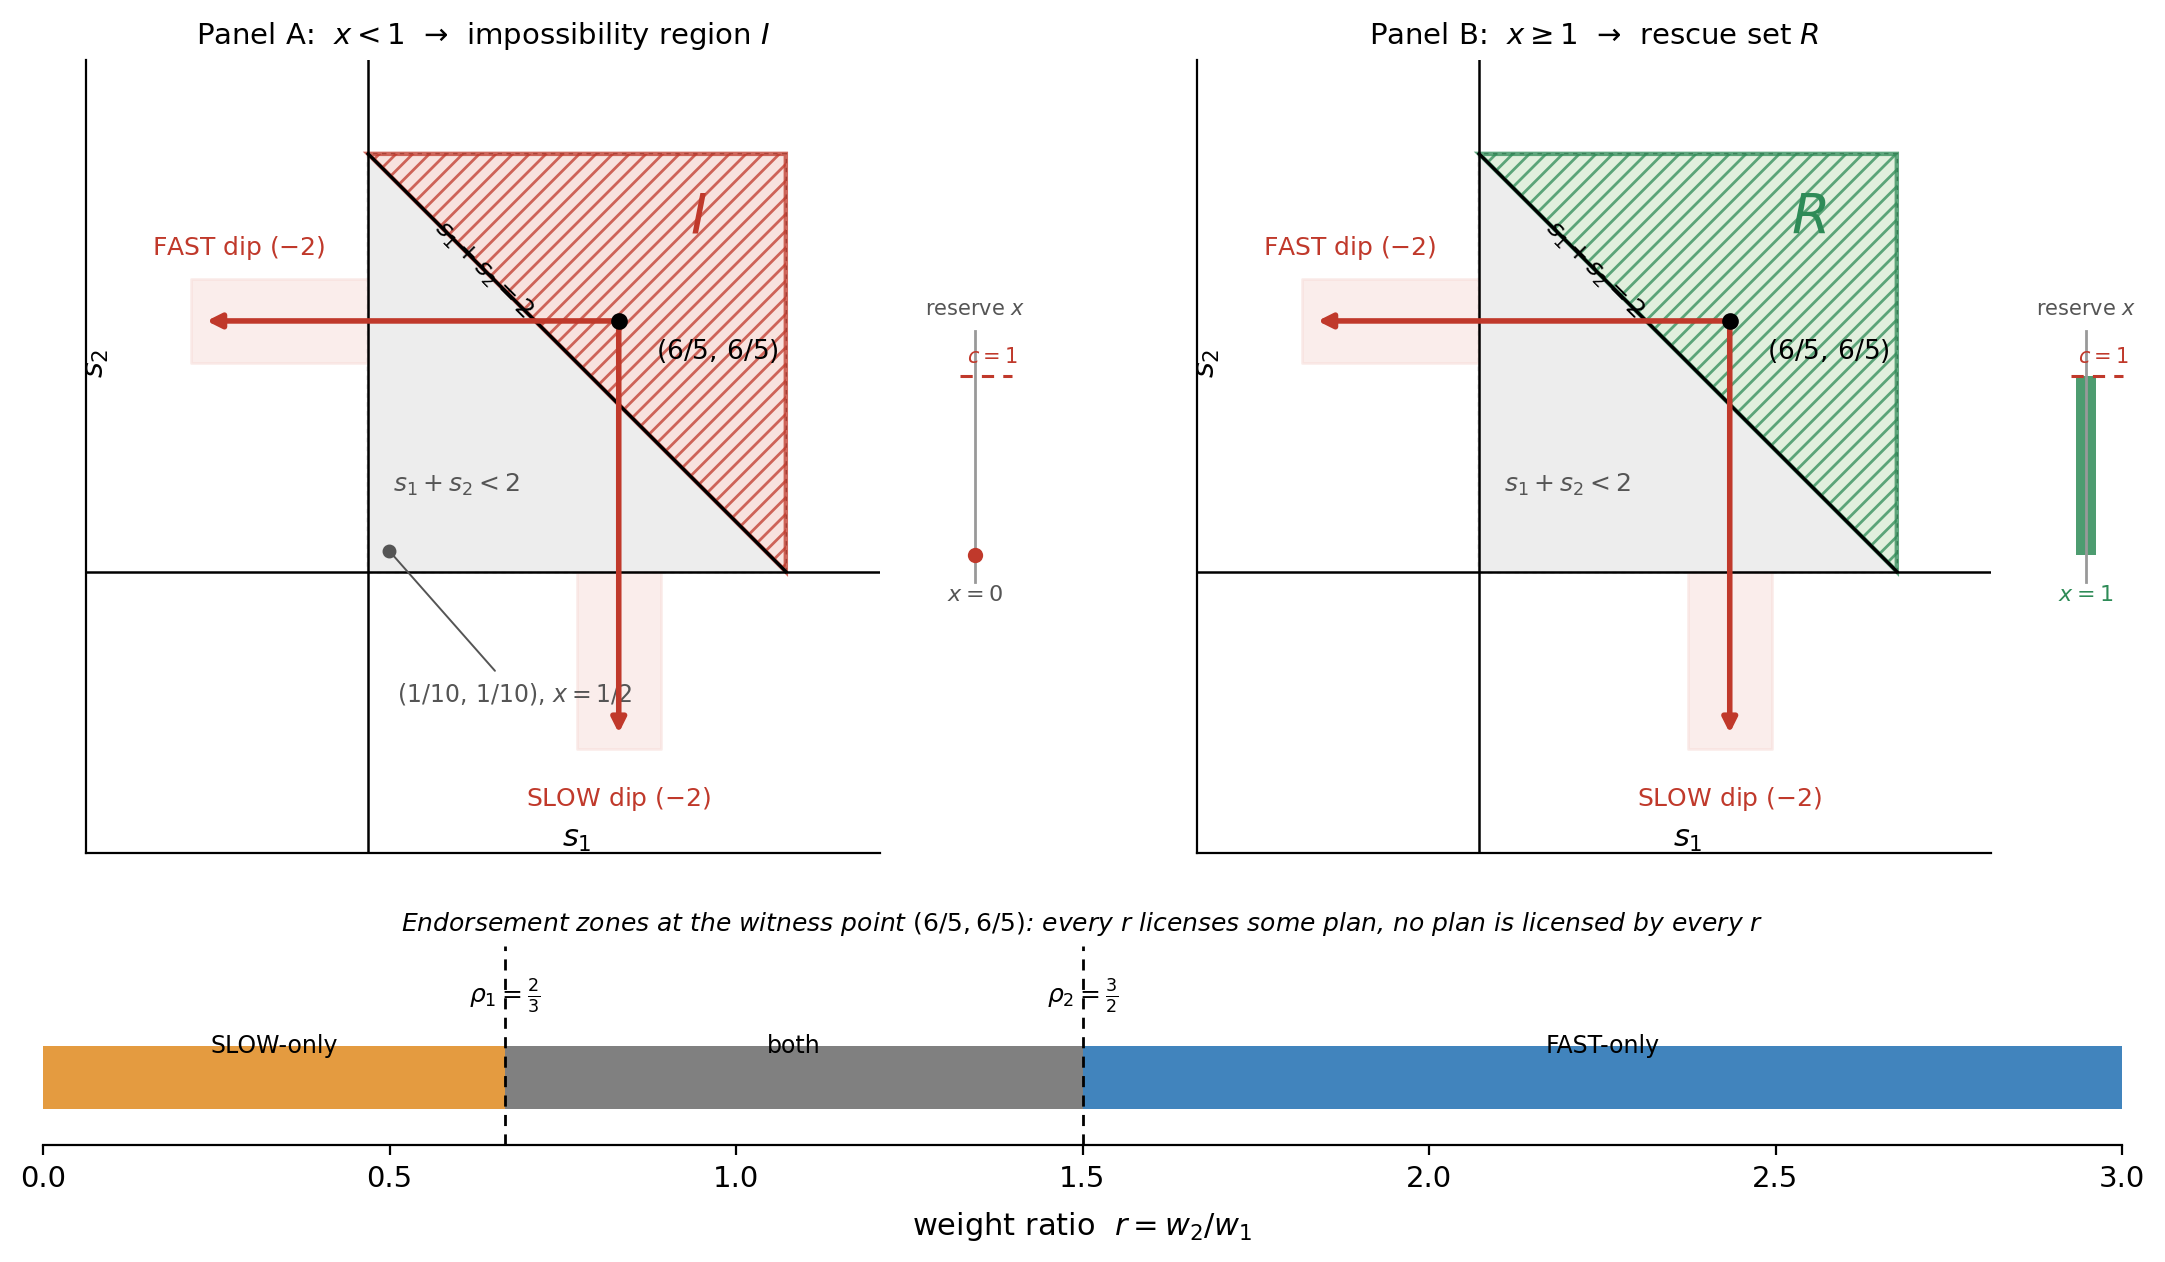
\includegraphics[width=\linewidth]{figs_p1/fig1_witness_v40.png}
\caption{The discrepancy triangle \(\mathcal{Q} = \{ s_1 < 2,\; s_2 < 2,\; s_1 + s_2 \ge 2 \}\) in the floor plane (boundary conventions as in Section 4.6). \textbf{Panel A (\(x < 1\)):} \(\mathcal{Q}\) is the impossibility region \(I = \mathrm{FP}_{\mathrm{agg}}\) --- every weighting licenses a plan, no plan satisfies the floors --- and the worst-case dip arrows show FAST (\(s_1 \to s_1 - 2\)) and SLOW (\(s_2 \to s_2 - 2\)) crossing the zero floors from the witness point \((6/5, 6/5)\). \textbf{Panel B (\(x \ge 1\)):} the same triangle is the rescue set \(R\), served by STAGED. Below the diagonal \(s_1 + s_2 = 2\), both assessments reject when \(x < 1\) and both accept when \(x \ge 1\). The reserve bars show the bridge stock \(x\) against the rescue cost \(c = 1\) (Panel A: \(x = 0\); Panel B: \(x = 1\)). The bottom strip records the endorsement zones at the witness point: SLOW-only for \(r < \rho_1 = \tfrac23\), both for \(\rho_1 \le r \le \rho_2 = \tfrac32\), FAST-only for \(r > \rho_2\). The reserve bars mark representative
slice values (Panel A: \(x = 0\), the impossibility-slice representative;
Panel B: \(x = 1\), at the rescue threshold); the dip arrows are
\(x\)-independent (the floor dynamics do not involve the reserve), and the
canonical witness point of Sections 4.6 and 6.3 sits at \(x = \tfrac12\),
between the drawn slices.}
\end{figure}

\begin{figure}[htbp]
\centering
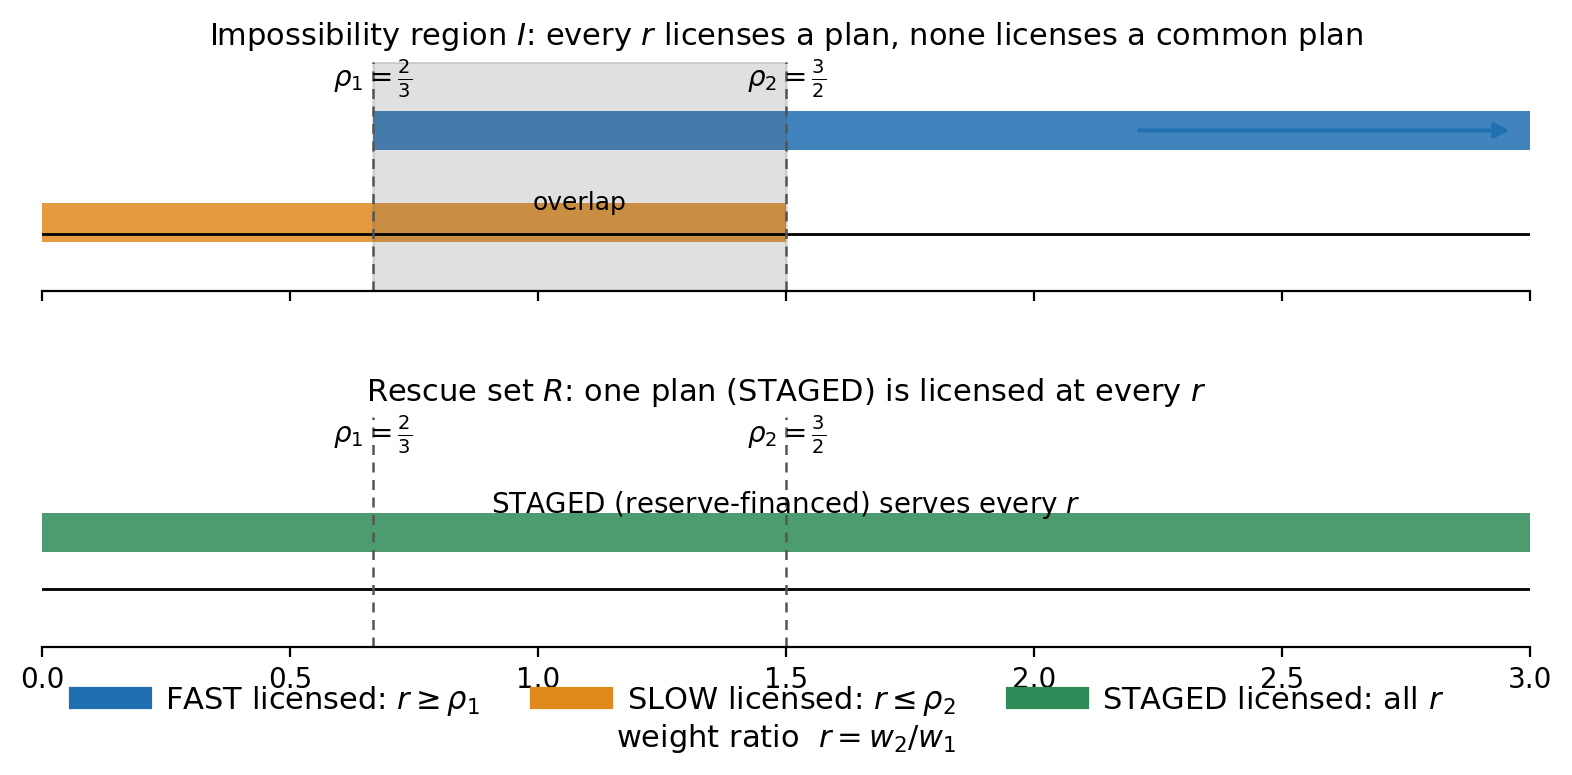
\includegraphics[width=0.98\linewidth]{figs_p1/fig2_weight_intervals_v35.png}
\caption{Weight-interval view at the witness point \((x, s_1, s_2) = (\tfrac12, \tfrac65, \tfrac65)\). FAST is licensed exactly for \(r \ge \rho_1 = \tfrac23\) and SLOW exactly for \(r \le \rho_2 = \tfrac32\). The two intervals together cover every weight ratio \(r \ge 0\), but neither covers it alone: every weight licenses a plan, no plan is licensed by every weight. On the rescue set, STAGED supplies the full interval and closes the gap.}
\end{figure}

\begin{figure}[htbp]
\centering
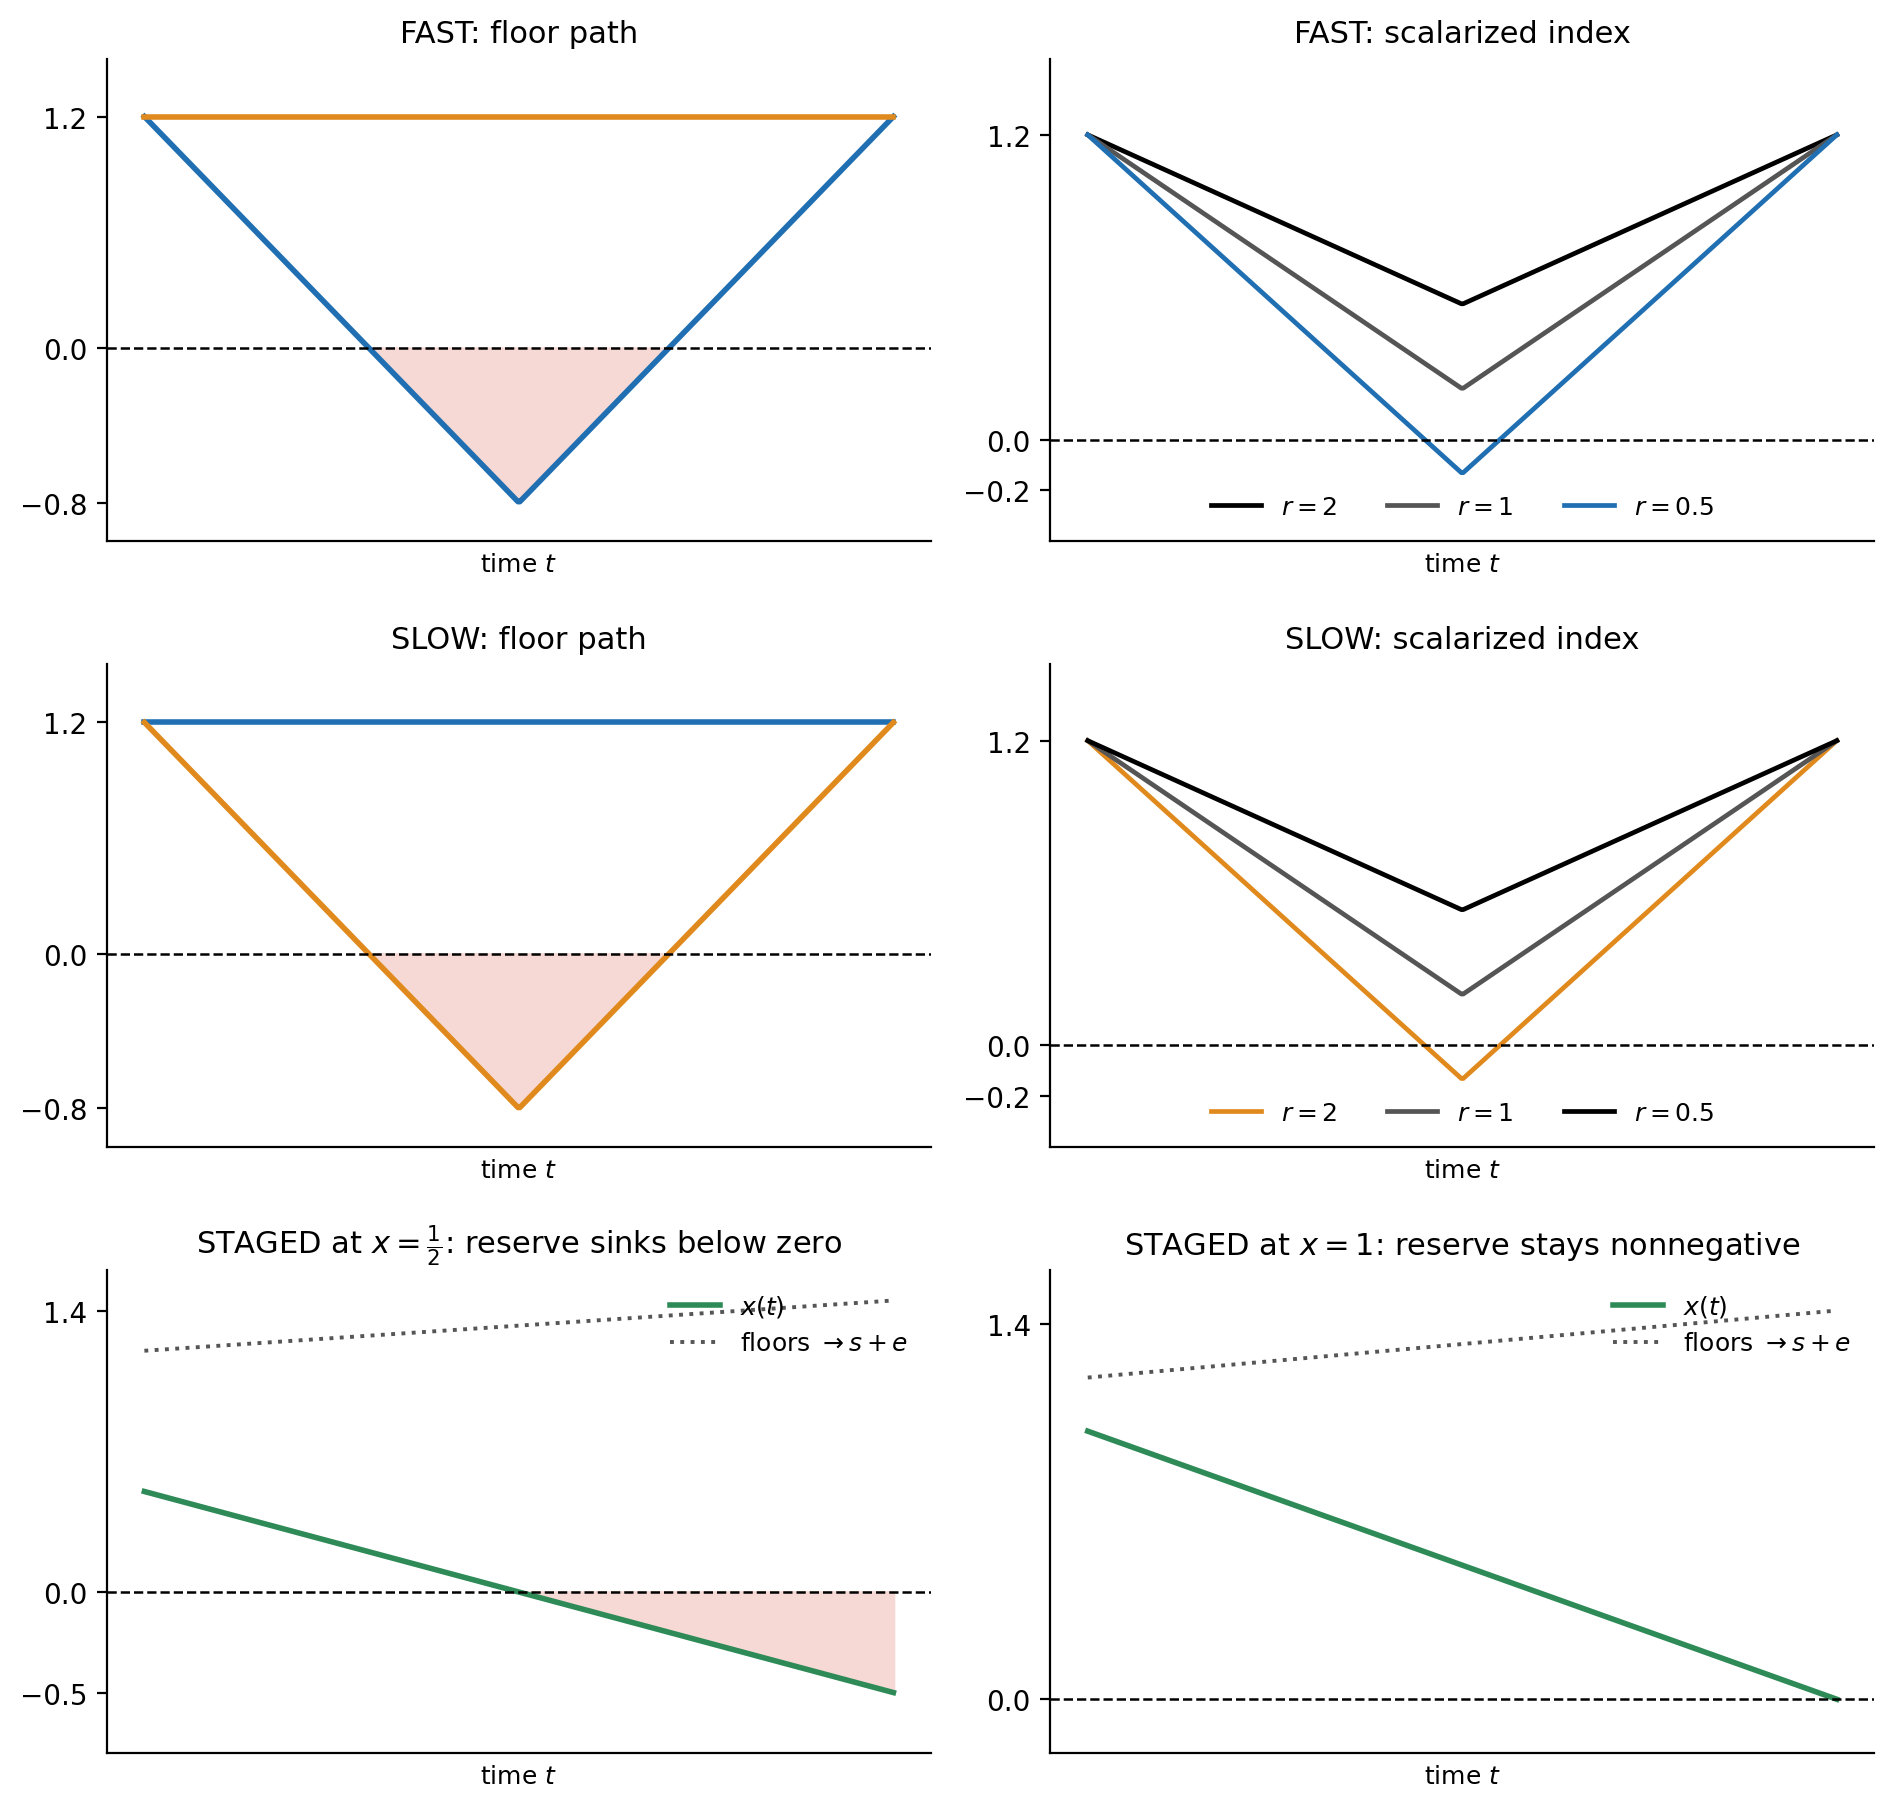
\includegraphics[width=0.98\linewidth]{figs_p1/fig3_path_view_v31.png}
\caption{Path view at the witness point. Rows: FAST, SLOW, STAGED under the worst-case disturbance; solid curves are the constrained paths, the dashed line the zero floor, and the colored curves the scalarized index for \(r \in \{2, 1, \tfrac12\}\). Under FAST (top row) the index stays nonnegative for \(r = 2\) and \(r = 1\) while \(s_1\) breaches its floor; under SLOW (middle row) the mirror holds. The only plan that protects both floors (bottom row, STAGED) consumes the reserve linearly: it is infeasible at \(x = \tfrac12\) and feasible at \(x = 1\), which is what separates the impossibility region from the rescue set.}
\end{figure}

\subsection{Propagation under hold-prefix
extension}\label{propagation-under-hold-prefix-extension}

This subsection asks whether the one-interval separation survives when
the horizon is lengthened by prepending hold intervals. Two results
delimit the answer. Remark 7 establishes persistence under a precisely
specified hold-prefix extension; Theorem 8 exhibits a two-stage datum on
which the gap is erased, showing the persistence claim is
architecture-conditional.

\textbf{Remark 7 (propagation).} \emph{Extend the witness datum to
\(m \ge 2\) review intervals by prepending hold intervals (sole action
HOLD: constant tube \(\{z\}\), successor \(\{z\}\), safe set \(S_0\);
the final interval carries the witness). Assume:}

\begin{itemize}
\tightlist
\item
  \emph{(H1) HOLD is available at every prefix state;}
\item
  \emph{(H2) the hold tube is exactly \(\{z\}\);}
\item
  \emph{(H3) the prefix safe sets contain the witness states;}
\item
  \emph{(H4) terminal and successor architecture labels are unchanged;}
\item
  \emph{(H5) no additional reset or disturbance branches are
  introduced.}
\end{itemize}

\emph{Then:}

\emph{(i) Hierarchy.} \emph{For every stage \(j\),}
\[\mathcal{V}^{\mathrm{typ}}_j \;\subseteq\; \bigcap_{w \in W_+} \mathcal{V}^{w}_j \;\subseteq\; \mathcal{V}^{\mathrm{phys}}_j.\]
\emph{This inclusion holds for every multi-interval typed exact-tube
datum; it is constraint monotonicity under backward induction.}

\emph{(ii) Persistence of strictness.} \emph{The stage-0 accepted
regions are the witness regions pulled back through the holds, so both
strictness witnesses of Theorem 5 persist under this hold-prefix
extension.}

\emph{(iii)} \emph{The displayed separation is not an artifact of the
one-interval framing for the constructed hold-prefixed datum. Strictness
for arbitrary multi-stage systems does not follow without a separate
persistence theorem: a later stage can erase the gap if every
aggregate-feasible state has a common typed-safe continuation, if the
weak and typed terminal sets coincide on the reachable subset, or if
actions couple across stages.}

\emph{Proof.} See Appendix B.

\textbf{Theorem 8 (erasure witness).} \emph{The propagation claim of
Remark 7 is architecture-conditional: there is a two-interval datum
whose single-interval truncation exhibits the acceptance gap and whose
two-stage extension erases it, through the terminal-coincidence
mechanism of Remark 7(iii).}

\emph{Proof.} See Appendix B.

The witness datum of Section 4.5 is not subject to this erasure. Its gap is
tube-driven: on \(I\) every member of the four-action menu violates the
stage-1 path constraint \(S_0\) itself (the two dips and the bridge
deficit of Theorem 5(7)), and a later stage cannot repair a violated
tube --- the stage-1 constraint is local to stage 1. Remark 7's safe
direction is secured by exactly the assumptions the erasure datum
violates (unchanged terminal architecture, no new branches). The two
results together delimit the persistence claim: hold-prefix extension
preserves the separation, arbitrary multi-stage extension does not, and
the erasure mechanisms of Remark 7(iii) are realizable.

\subsection{Machine verification}\label{machine-verification}

Proposition 3, Proposition 4, Theorem 5, Theorem 6, Remark 7, Theorems
8--9, and Proposition 10 are proved in Appendices A--C, and Proposition 11
in Appendix C. An accompanying software artifact (deterministic exact-integer arithmetic; no floating point, tolerances, or randomness) checks the finite rational instance of Proposition 3, Proposition 4, Theorem 5, and Remark 7: the action classifications, the region identities, and the accepted-set identities on a \(31^3 = 29{,}791\)-state grid over \((x, s_1, s_2)\), with a finite verification set containing the critical weight ratios \(\rho_1, \rho_2\) and their midpoint for every enumerated grid state. All 25 checks pass and re-execution reproduces them exactly; they are enumerated in the Supplementary Material (S8). This grid verifier is distinct from the software companion's separate 24-check benchmark suite, which re-derives the Section 6.3 fishery instantiation; the two counts index different check lists, not a disagreement.

\noindent\begin{tabular}{@{}
  >{\raggedright\arraybackslash}p{(\columnwidth - 4\tabcolsep) * \real{0.3333}}
  >{\raggedright\arraybackslash}p{(\columnwidth - 4\tabcolsep) * \real{0.3333}}
  >{\raggedright\arraybackslash}p{(\columnwidth - 4\tabcolsep) * \real{0.3333}}@{}}
\toprule\noalign{}
\begin{minipage}[b]{\linewidth}\raggedright
Claim layer
\end{minipage} & \begin{minipage}[b]{\linewidth}\raggedright
What is established
\end{minipage} & \begin{minipage}[b]{\linewidth}\raggedright
By what
\end{minipage} \\
\midrule\noalign{}
Continuum statements & Exact identities and inequalities on the witness datum & Appendices A--C \\
Finite rational instance & Classifications on the enumerated grid & Deterministic computation \\
Empirical claims & None in this article & --- \\
\bottomrule\noalign{}
\end{tabular}

The finite grid does not by itself prove the continuum identities; it
validates the symbolic classification on the enumerated instance.

\subsection{Menu convexification: the blend
family}\label{menu-convexification-the-blend-family}

The action space is the finite menu \{FAST, SLOW, STAGED,
NO-SWITCH\} of deterministic actions; fractional or alternating policies
are not members of it. The convexification instrument is the blend
family: for each \(\delta \in (0,1)\), the action BLEND\(_\delta\) is
the \emph{convexified action} obtained by fractional allocation of the
primitive control flows,
\(u_\delta = \delta\, u_{\mathrm{FAST}} + (1-\delta)\, u_{\mathrm{SLOW}}\);
by linearity of the flow map its worst-case tube is the pointwise convex
combination of the two primitive worst-case tubes and its successor the
convex combination of the two successors. This is menu convexification
at the level of control inputs --- an explicit model assumption, not the
time-sharing of discrete actions in alternation.


\noindent\textbf{A limitation to state before the theorem.} The blend
family is an explicitly defined convexified control map --- an instrument
of the abstract witness datum, not by itself a claim that fractional plans
are available anywhere. Convexification must be demonstrated from the
model equations (as here, by linearity of the flow map in the control) or
carried explicitly as a management assumption; and a blended control
requires physical and institutional implementability --- fractional
allocation of effort, quota, or seasonal resolution, with monitoring and
enforcement --- before Theorem 9 is applied to a real plan menu. The
theorem is a statement about certification relative to the convexified
menu; the menu's availability is external data (the fourth design test of
Section 5.5 and the instruments of Section 5.6).

\textbf{Theorem 9 (blend collapse).} \emph{On the witness datum of
Section 4.5, over initial states \(X_0\):}

\emph{(i)} \emph{BLEND\(_\delta\) is typed-admissible at \(z\) exactly
when}
\[\delta \in \left[\,1 - \frac{s_2}{2},\; \frac{s_1}{2}\,\right] \cap [0,1],\]
\emph{an interval nonempty exactly when \(s_1 + s_2 \ge 2\) (a singleton
at equality), independent of \(x \ge 0\) and of the weight; the
intersection with \([0,1]\) is the convex-combination domain of
\(\mathrm{BLEND}_\delta\) and is inactive on \(\mathcal{Q}\), where
\(0 < 1 - s_2/2 \le s_1/2 < 1\) automatically.}

\emph{(ii)} \emph{The typed acceptance set of the menu augmented by the
blend family is exactly the compensatory region:}
\[\mathcal{V}_{\mathrm{typ}}^{\mathrm{blend}} \;=\; \{ x \ge 1 \} \cup \{ s_1 + s_2 \ge 2 \} \;=\; \mathcal{V}_{\mathrm{weak}}.\]
\emph{Convexification of the menu collapses the acceptance gap:
\(\mathrm{FP}_{\mathrm{agg}}\) vanishes under the augmented menu, and
the blend family reaches exactly the compensatory region and nothing
beyond --- on
\(\mathcal{V}_{\mathrm{phys}} \setminus \mathcal{V}_{\mathrm{weak}}\) no
blend is typed-admissible.}

\emph{(iii)} \emph{The admissible window depends on the state through
\((s_1, s_2)\) alone: a single \(\delta\) serves every weight
\(w \in W_+\). On the impossibility region the blend is therefore the
common action that no member of the finite menu supplies --- the
acceptance gap is a property of the deterministic menu, not of the
doctrines.}

\emph{Proof.} See Appendix B.

\emph{Remark.} The collapse is exact and weight-independent: a single
convexified plan serves every assessor on \(I\), where the per-weight
plans of Theorem 5(6) necessarily differ. The nonconvexity at work is
menu geometry --- the finiteness and determinism of the action space ---
not the Pareto-frontier geometry under which weighted sums fail to reach nonconvex frontier parts (Das and Dennis, 1997); the two mechanisms are distinct. The structure is precisely that of
pure-versus-mixed strategies in the assessor--planner game (von Neumann,
1928; Sion, 1958): with the planner picking an action, the assessor a
weight, and the payoff the worst-case aggregate, common-plan acceptance
is the pure-strategy value and per-weight acceptance the mixed value,
the gap being the pure-strategy duality gap that the convex (mixed)
extension closes. The two-player reach/avoid formulation of such games is the discriminating kernel of Cardaliaguet (1996), with numerical treatment in Cardaliaguet, Quincampoix, and Saint-Pierre (1999). This is also the here-and-now versus wait-and-see
separation of adjustable robust optimization (Ben-Tal et al., 2004).

\textbf{A class-conditional caveat on the blend collapse.} Theorem 9's
window is computed under the action-indexed disturbance convention of
Section 4.5, and it is class-conditional: under the common-shock class
of Section 5.9 the window is nonempty exactly on \(\{ s_1 \ge \delta,\;
s_2 \ge \delta,\; s_1 + s_2 \ge 3/2 + 2\delta \}\) (at the datum's event
depth \(\delta = 1/2\): \(\{ s_1 \ge 1/2,\; s_2 \ge 1/2,\; s_1 + s_2
\ge 5/2 \}\), against the action-indexed \(\{ s_1 + s_2 \ge 2 \}\) of
Theorem 9(i)). The common-shock acceptance gap --- which survives the
shared shock (Theorem M1, Section 5.9) --- is therefore \emph{not}
blend-closed on the fragile band \(s_1 + s_2 \in [2, 5/2)\): the witness
\((\tfrac12, 1, 1)\) is a common-shock gap state with \emph{no}
admissible blend, while every common-shock gap state with
\(s_1 + s_2 \ge 5/2\) has one (Theorem M3 there; the coupled variant,
by contrast, is blend-closed --- the fragility is class-conditional). An
agency that would otherwise invoke Theorem 9's collapse at a shallow
common-shock gap state cannot: the blended menu itself is inadmissible
there.

\subsection{The converse: discrete time-sharing does not erase
the
gap}\label{the-converse-discrete-time-sharing-does-not-erase-the-gap}

\textbf{Proposition 10 (sequential time-sharing does not erase the gap).}
\emph{On the witness datum of Section 4.5, let a sequential time-shared
policy alternate between FAST and SLOW over the interval, so the set of
visited states is the union of the two primitive worst-case tubes. Then
such a sequential policy is typed-admissible if and only if
\(s_1 \ge 2\) and \(s_2 \ge 2\); on the impossibility region \(I\)
(where \(s_1 < 2\), \(s_2 < 2\), \(s_1 + s_2 \ge 2\)) no such policy is
typed-admissible, and the acceptance gap therefore survives discrete
time-sharing.}

\emph{Proof.} See Appendix B.

\emph{Remark.} Together Proposition 10 and Theorem 9 delimit the notion
of mixing precisely: continuous convexification --- fractional
allocation of control flows --- closes the acceptance gap exactly at the
compensatory region \(s_1 + s_2 \ge 2\), whereas discrete time-sharing
--- alternation in time, whose visited set is the union of the action
tubes --- closes it only where the two dips are independently subsumed,
\(s_1 \ge 2\) and \(s_2 \ge 2\).

On the regime \(s_1 + s_2 \ge 2\) with
\(\min(s_1, s_2) < 2\) (which contains the impossibility region) the gap survives sequential time-sharing and closes only under convexification, so the structural character of the gap is a property of
the \emph{convexity of the action space}, not of the assessment doctrine
and not of temporal sharing as such. A terminological precision is
required here. In the language of relaxed controls, the collapse theorem
is a statement about the convexified (relaxed) action program. The
converse is a statement about discrete, plan-granular alternation at
full strength: each primitive plan is held for a whole sub-interval, so
the visited set is the union of the primitive tubes. That stipulated
visited set is the pointwise worst case over alternation schedules --- a
literal rate-preserving fine-grained alternation visits sub-ranges of it
--- so the impossibility established here is scoped to the worst-case
alternation. It is not a
statement about the chattering limit of classical relaxed-control
theory (Filippov; Warga): infinitesimally fast switching recovers the
convexified trajectory and is therefore subsumed by Theorem 9, not
distinct from it. What fails to erase the gap is alternation at finite
rate and plan granularity, not rapid switching.

\begin{center}\rule{0.5\linewidth}{0.5pt}\end{center}

\section{Interpretation}\label{interpretation}

\subsection{The doctrinal reading}\label{the-doctrinal-reading}

The scalarized operators \(\{E_w\}_{w \in W_+}\) formalize \textbf{one}
compensatory assessment doctrine. The doctrine comprises: a single
aggregate index \(w \cdot s\); nonnegative scalarization weights on
capital forms; substitution across floors permitted at those weights;
and disturbances respected. We refer to this as \emph{the scalarized
aggregate doctrine as formalized here}, not as ``weak sustainability''
simpliciter. The weak-sustainability literature is broader than this
operator: it encompasses aggregate wealth, constant total capital,
nondeclining comprehensive consumption, substitutability assumptions,
discounting, shadow prices, and intertemporal investment conditions
(Neumayer, 2013; World Bank, 2011; Boos, 2015; Dasgupta and M\"aler, 2000;
Asheim, 1994). Likewise, strong sustainability is not always equivalent
to requiring every stock coordinate to remain nonnegative at every
instant. Critical-natural-capital frameworks may use thresholds, safe
operating spaces, irreversibility, resilience, or minimum-service
conditions (Ekins et al., 2003; Rockstr\"om et al., 2009; Raworth, 2012;
Doyen and Gajardo, 2020). The typed
operator \(E_{\mathrm{typ}}\) is a formal idealization of the
separately-binding-floor reading, in the same sense that the scalarized
operators idealize one aggregation doctrine. The typed operator is the
coordinate-wise criterion --- each floor is required to hold separately ---
and the scalarized family is the compensatory criterion; the two vocabularies
name the same operators, with \emph{typed} denoting the framework object and
\emph{coordinate-wise} its constraint structure.

Within this precise scope, Theorem 5 reads as follows. The two
formalized doctrines can disagree on the same transition datum, with the
same robustness standard and the same action set, in the direction
compensatory-accepts / noncompensatory-rejects, on a relatively open
region. The disagreement is not an artifact of one bad weight: every
weight accepts, each licensing a different physical transition. The
plans are genuinely different transitions (FAST and SLOW violate
different floors at different times), which is the dynamic formalization
of substitution across floors. By Proposition 3(ii), the precise seat of
the disagreement is the noncommutativity of ``choose an action'' with
``for all weights.''

At the static level the full-cone aggregate is lossless (Remark 2), so the compensatory doctrine's limitation is not the existence of an aggregate index but the \emph{policy dependence} of the aggregate-feasible transition: the index certifies a set of transitions, none of which the noncompensatory assessment accepts. The two
quantifier orders also carry an information reading.
\(\exists a\, \forall w\) is a commitment made before the weight is
known --- the strong doctrine's robustness demand --- while
\(\forall w\, \exists a_w\) lets the action be chosen after the weight
is observed. On the witness, the acceptance gap between the two orders
measures the value of information about the assessment weight. Theorem 9 qualifies this reading: a single convexified blend serves every weight on the impossibility region, so the value of information reflects the finite deterministic menu rather than the weight information itself. Proposition 10 sharpens the point: the value of information is removed by convexifying the action space, not by sharing actions in time --- under discrete time-sharing the gap (and
hence the value of information about the weight) survives on the
impossibility region.

Throughout, we use ``nonnegative scalarization weights'' for elements of
\(W_+\) and reserve the word ``prices'' for the interpretive discussion.
Actual prices may be strictly positive, endogenous,
dynamically determined, state-dependent, or dimensionally heterogeneous,
and the theorems require none of those properties. The operators are
linear scalarizations with weights fixed over the review interval.
Nonlinear aggregate indices --- CES-type substitutability or endogenous,
state-dependent weighting of the kind that diverges near zero-stock
boundaries --- are different assessment operators, and the theorems
claim nothing for them. Section~\ref{substitutability-spectrum} begins the
programme of establishing what can be claimed for the CES family on the
witness datum.

\subsection{Positioning against established
theory}\label{positioning-against-established-theory}

The backward recursion of Section 3 is
a typed instance of established robust-predecessor, reach-avoid,
capture-basin, and hybrid-reachability constructions (Aubin, 1991;
Aubin, Bayen, and Saint-Pierre, 2011; Saint-Pierre, 1994; Lygeros,
Tomlin, and Sastry, 1999); the fixed-point and algebraic character of these objects is developed in Aubin and Catt\'e (2002). Viability methods are likewise developed in natural-resources management, with fisheries a canonical application (De Lara and Doyen, 2008; Doyen et al., 2012). Proposition 3(i) is constraint-set
monotonicity of viability kernels and reachability sets (Aubin, 1991;
Frankowska, 1989). Static scalarization limitations --- weighted sums that cannot
reach nonconvex parts of Pareto fronts (Das and Dennis, 1997) --- act
through frontier geometry under a single optimization, a mechanism
distinct from the action-quantifier mechanism established here. The
per-literature details --- the commensurability foundation
(Martinez-Alier, Munda, and O'Neill, 1998), the maximin and indicator
formulations of strong sustainability (Martinet, 2011; Cairns and
Martinet, 2014; Doyen and Gajardo, 2020), and the compensability mapping
in multi-criteria decision analysis --- including the outranking approach
PROMETHEE, whose compensatory properties the cited analysis dissects
(Cinelli, Coles, and Kirwan, 2014; Sch\"ar, Pohl, and Geldermann, 2025) --- are collected in the
Supplementary Material (S10).

Against this background, the finite-menu characterization of
Section 4.4 is the general form, of which the witness separation
(Theorem 5) and the blend collapse (Theorem 9) are the instances.

To our knowledge, no explicit exact-tube witness for this dynamic
separation in a compensatory/noncompensatory assessment setting is
reported in the literature. We do not assert priority over the
elementary quantifier fact
\(\exists a\, \forall w \neq \forall w\, \exists a_w\), which is
standard. Whether an equivalent dynamic separation appears in adjacent
literatures (multi-objective robust control, viability theory,
multi-criteria decision analysis) is not established either way.

\subsection{A translation guide for readers from neighbouring
fields}\label{translation-guide}

Because the paper sits at a confluence --- multi-criteria decision analysis
and operations research, control theory and viability, environmental
modelling and governance --- Table~\ref{tab:translation} translates its
central objects into each neighbouring literature's working vocabulary. The
readings are exact correspondences of mathematical role, not analogies: the
theorems are venue-neutral, and a reader may enter through any column.

\begin{table}[htbp]
\centering
\small
\caption{Terminology map: this paper's objects read from three neighbouring
vocabularies.}
\label{tab:translation}
\begin{tabular}{@{}p{2.55cm}p{3.85cm}p{3.55cm}p{4.55cm}@{}}
\toprule
 & \textbf{MCDM / operations research} & \textbf{Control / viability theory} & \textbf{Environmental modelling / governance} \\
\midrule
Typed floors \(s_i \ge 0\), enforced path-wise &
coordinate-wise (vector) criteria; per-criterion lower bounds along the whole path &
state constraints; safe set \(\mathcal{V}\); path (tube) constraints &
planetary boundaries; safe operating spaces; regulatory floors (e.g., a biomass limit reference point) \\
\addlinespace
Scalarized operator \(E_w\) &
weighted-sum acceptance; weight space \(W_+\) &
scalarized robust constraint on an aggregate output &
composite sustainability index; the assessment dashboard \\
\addlinespace
Licensing thresholds \(\rho_1, \rho_2\) &
weight intervals of acceptance; weight-space robustness of a recommendation &
parameter-dependent feasibility margins &
indicator weighting schemes; stakeholder weight elicitation \\
\addlinespace
Acceptance gap \(\mathrm{FP}_{\mathrm{agg}}\) &
scalarization error: accepted by some weighted sum, infeasible coordinate-wise &
gap between the scalarized program and the viability kernel &
the aggregation illusion: an index certifying what the floors reject \\
\addlinespace
Rescue set \(R\); threshold \(\kappa^*\) &
alternatives repairable by a budgeted side payment &
reachability under an auxiliary resource input &
transition finance: adjustment funds, fleet buy-backs \\
\addlinespace
Impossibility region \(I\) &
robust infeasibility: rejected at every weighting &
empty common safe-action set over the belief; kernel exclusion &
hidden collapse zone: index nonnegative, floor crossed mid-transition \\
\addlinespace
Blend collapse (Thm 9) vs.\ time-sharing (Prop 10) &
randomized (mixed) strategies vs.\ deterministic sequencing &
relaxed (convexified) controls vs.\ plan-granular alternation (not the
chattering limit) &
blended policy portfolios vs.\ alternating policies \\
\addlinespace
Exact-tube semantics &
robust path-wise feasibility over a scenario set &
viability tubes; worst-case reachability &
avoiding transient breaches (e.g., extinction vortices during a transition) \\
\bottomrule
\end{tabular}
\end{table}

\subsection{Scope delimitations}\label{scope-delimitations}

\begin{itemize}
\tightlist
\item
  \textbf{No separation on every datum.} Where a single action is safe
  for all weights, the assessments coincide. The theorem is an existence
  separation with an open region, plus the always-valid hierarchy and
  localization.
\item
  \textbf{No infinite-horizon, stochastic, partial-observation, or
  endogenous-event extension.} All statements are for finite-horizon exact-tube data with specified disturbance sets.
\item
  \textbf{No claim that the full nonnegative cone is the only reasonable
  weight family.} Proposition 4 shows that restricting the family
  enlarges the compensatory accepted set, so the full cone is the strictest compensatory reading, and the separation persists a fortiori for restricted families.
\item
  \textbf{No welfare claim about prices.} The weights model an
  assessment doctrine, not a normative endorsement.
\item
  \textbf{No empirical transfer.} The theorems concern assessment operators on a specified datum and imply no empirical claim about any resource system.
\item
  \textbf{No claim that \(\mathcal{V}_{\mathrm{weak}}\) is the
  genuine-savings or inclusive-wealth criterion.} The operator is the
  strictest compensatory reading (every weight, each licensing an
  action). The genuine-savings literature's criterion is a different
  object, and the witness's reserve stock is excluded from the weighted aggregate by construction (Section 4.5), not by consequence of aggregation. If the reserve entered the aggregate with positive weight, the gap could shrink or disappear; the separation isolates the case in which the aggregate measures the service floors while the reserve is a separate policy instrument.
\item
  \textbf{No absolute impossibility.} The impossibility region is a negative certificate relative to the specified four-action menu; with a larger menu it can shrink or vanish (see the completeness requirement in Section 5.7).
\item
  \textbf{No universal doctrinal ranking.} The inclusion
  \(\mathcal{V}_{\mathrm{typ}} \subseteq \mathcal{V}_{\mathrm{weak}} \subseteq \mathcal{V}_{\mathrm{phys}}\)
  is a theorem about the defined operators under common action and
  disturbance classes, common safe-set inclusion, common horizon, common
  tube semantics, and common terminal condition. It does not establish a
  universal ranking of endpoint, weak, and strong sustainability
  doctrines.
\item
  \textbf{No separation under coupled all-floor shocks.} The witness
  disturbance convention is action-indexed (Section 4.5): each action's
  worst case is its own characteristic dip. A datum whose disturbance
  class couples simultaneous dips across all floors of every action
  degenerates the per-weight licensing structure --- the principal
  actions fail together and the compensatory/noncompensatory divergence
  collapses into universal rejection. The exact statement, computed in
  Section 5.9, is reading-conditional and depth-dependent: under the
  additive reading the rejection is universal on \(I\) at the datum's
  full magnitude, with the exact depth boundary \(\delta = 5/4\) below
  which deep-\(I\) states survive (witness \((\tfrac12,
  \tfrac{19}{10}, \tfrac{19}{10})\) at heatwave magnitude) and with the
  separation relocating --- not vanishing --- at full magnitude (the
  coupled gap \(\{ x < 1,\; 2 \le s_1 < \tfrac72,\; 2 \le s_2 <
  \tfrac72,\; s_1 + s_2 \ge \tfrac{11}{2} \}\), witness \((\tfrac12,
  3, 3)\)); under the replace reading the principal actions fail
  together under one weight-independent requirement and what collapses
  is the typed/weak distinction itself (\(\mathcal{V}_{\mathrm{weak}} =
  \mathcal{V}_{\mathrm{typ}}\), Theorem CT there), with acceptance ---
  not rejection --- surviving at \(\{ s_1 \ge 2,\; s_2 \ge 2 \} \cup
  \{ x \ge 1,\; \min(s_1, s_2) \ge \tfrac{15}{8} \}\), a strictly
  more demanding reading (the witness \((\tfrac12, 3, 1)\) is
  action-indexed typed-accepted yet fully rejected under it). The
  separation is exhibited for, and scoped to, the specified
  action-indexed class: the witness datum assumes separable transition risks, with each plan exposing a different floor to its own adverse disturbance. That the coupled regime is not a remote possibility is indicated by evidence that planetary-boundary processes interact and amplify one another (Lade et al., 2020).

\medskip

\noindent The disturbance-class scoping, organized
(Table~\ref{tab:disturbance}): the witness's action-indexed separable
class is one of three regimes; the second's verdict is the common-shock
computation of Section 5.9 (Theorem M1: the gap survives the shared
shock, reduced by the exact \(1/2\)-cut, with licensing thresholds
unshifted on the surviving region) --- a verdict computed, not asserted,
exactly as the regime demands; the third is the universal-rejection
collapse stated above, refined there into two exact reading-conditional
theorems (M4 and CT).

\begin{table}[htbp]
\centering
\small
\caption{Disturbance regimes on the witness datum. The middle row's
verdict is the exact common-shock computation of Section 5.9 (Theorem
M1); the third row's exact statement is reading-conditional (Theorems
M4 and CT there).}
\label{tab:disturbance}
\begin{tabular}{@{}p{3.1cm}p{4.0cm}p{6.3cm}@{}}
\toprule
Regime & Disturbance class & Separation status \\
\midrule
(i) Action-indexed separable & each action's worst case is its own characteristic dip in the coordinate it moves (Section 4.5) & proven: the witness datum exhibits the acceptance gap (Theorem 5) \\
(ii) Common biomass shock & one shared shock strikes the same floor coordinate of every plan & computed (Theorem M1, Section 5.9): the gap \emph{survives} the common shock, reduced by the exact \(1/2\)-cut --- every action-indexed gap state with \(\min(s_1, s_2) < 1/2\) weak-rejects --- with licensing thresholds unshifted on the surviving region; the canonical datum remains a member \\
(iii) Coupled all-floor shocks & simultaneous dips across all floors of every action & reading-conditional (Theorems M4 and CT, Section 5.9): additive --- universal rejection exact on \(I\) at the datum's full magnitude, depth-dependent below the exact boundary \(\delta = 5/4\), the gap relocating (not vanishing) at full magnitude; replace --- the per-weight licensing structure degenerates to one weight-independent requirement, the actions fail together, and the typed/weak distinction itself collapses (\(\mathcal{V}_{\mathrm{weak}} = \mathcal{V}_{\mathrm{typ}}\)), with acceptance --- not common rejection --- surviving (this section; Lade et al., 2020, on boundary interactions) \\
\bottomrule
\end{tabular}
\end{table}

\item
  \textbf{Convexification of the menu.} Fractional action policies are
  not members of the action space, and every stated separation is scoped
  to the finite deterministic menu. Theorem 9 resolves the convexification question: the blend family collapses the typed acceptance set exactly onto the compensatory
  region, so the separation is a property of the deterministic menu, not
  of the doctrines --- menu geometry, distinct from the Pareto-frontier
  geometry of scalarization limits (Das and Dennis, 1997). The
  associated delimitation (Proposition 10) is that discrete time-sharing
  does not effect the same collapse: on the impossibility region the gap
  survives alternation in time, so the structural character of the separation is due to the convexity of the action space, not to temporal sharing.
\end{itemize}

\subsection{Indicator validity: four design tests}\label{indicator-validity}

The separation theorem implies that a composite indicator can be
statically lossless yet dynamically unsound as a
transition-certification device. For indicator developers the theorem
converts into four design tests --- the questions an indicator's
documentation must answer before the index is used to certify a
transition. Each test is a reading of a proved statement; none is a
heuristic.

\begin{enumerate}
\tightlist
\item
  \textbf{Static losslessness.} Does the aggregate preserve component
  violations at a fixed trajectory for the declared weight family? At the
  full cone, yes (Remark 2); for a restricted family, the test is to
  characterize the component violations the restricted family can miss
  (Proposition 4). An index that fails this test fails statically; the
  separation of Section 4 is the further, dynamic failure.
\item
  \textbf{Protocol quantifiers.} Does the certification rule require a
  common plan (\(\exists a\, \forall w\)) or permit weight-adaptive plan
  selection (\(\forall w\, \exists a_w\))? If the latter --- Protocol 2
  of Table~\ref{tab:protocols} --- the indicator is exposed to the
  acceptance gap on exactly the region Theorem 5 exhibits.
\item
  \textbf{Path-wise observability.} Is the index evaluated along the
  full tube, or only at audited endpoints? Endpoint evaluation is the
  weakest operator of the chain (Section 3.1) and cannot detect transient
  breaches --- mid-interval floor crossings that are invisible at
  snapshots (\(E_{\mathrm{end,typ}}\) versus \(E_{\mathrm{typ}}\) on
  the witness datum).
\item
  \textbf{Menu completeness and convexity.} Is the plan menu exhaustive,
  and are blended (convexified) plans implementable? Negative feasibility
  verdicts are menu-relative (Section 5.4), and the gap is a property of
  the deterministic menu that convexification collapses exactly (Theorem
  9, Proposition 10); the availability of the convexified menu is
  external data that the indicator's documentation must declare.
\end{enumerate}

\textbf{A consolidated practitioner checklist.} For an agency using a
composite dashboard to certify a sustainability transition, the four
tests and the theorems behind them operationalize as ten audit points:

\begin{enumerate}
\tightlist
\item
  \textbf{Object of certification:} state what is being certified --- a
  static state, an endpoint, or the existence of a path-wise safe
  management plan.
\item
  \textbf{Binding floors:} list the floors that are legally binding,
  irreversible, or lack verified substitutability; these require
  noncompensatory (Protocol 4) treatment.
\item
  \textbf{Policy quantifier:} declare whether the approval rule assumes
  one robust plan or lets the plan adapt to the weighting.
\item
  \textbf{Weight-dependent plans:} if weight-adaptive, report the
  management plan associated with each relevant weight range (the
  licensing thresholds \(\rho_1, \rho_2\) of Theorem 5(6) are the
  pattern).
\item
  \textbf{Path-wise evaluation:} evaluate the floors along the full
  transition, not only at assessment snapshots (the endpoint operators
  are the weakest of the chain; Section 3.1).
\item
  \textbf{Disturbance structure:} specify whether shocks are common to
  all plans, action-indexed, or correlated across floors
  (Table~\ref{tab:disturbance}); the separation's scope rides on the
  class.
\item
  \textbf{Menu completeness:} acknowledge that negative feasibility
  results are menu-relative unless the action space is demonstrably
  exhaustive (Section 5.4).
\item
  \textbf{Blended policies:} do not infer convexification from
  mathematical convenience; verify that fractional effort or quota
  allocation is administratively implementable (the limitation stated
  before Theorem 9).
\item
  \textbf{Rescue margins:} if a resource-controlled action exists, report
  the minimum increment \(\kappa^*\) that converts impossibility into
  rescue (Section 5.7).
\item
  \textbf{Mandatory reporting:} require that component trajectories and
  their minimum margins be reported alongside the aggregate index, so the
  typed verdict can be independently reconstructed (the minimum report of
  Section 5.6).
\end{enumerate}

\subsection{Policy implications}\label{policy-implications}

The separation theorem has four implications.

\textbf{First.} Aggregate indices alone cannot certify noncompensatory
transition safety under the present assessment semantics. A scalarized
assessment can certify its own criterion --- aggregate feasibility; what
it cannot certify is typed safety unless an additional bridge theorem is
supplied. This follows from Theorem 5: the compensatory accepted set
strictly contains the noncompensatory accepted set, and the excess
region is where the two criteria diverge.

\textbf{Second.} When the typed recursion identifies an admissible
rescue action whose feasibility is controlled by a resource margin,
investment in that margin is a candidate remedy; reweighting alone cannot substitute for it on the witness datum (Section 5.7). This applies where a resource-controlled rescue action exists; it is not a universal policy claim.

\textbf{Third.} Per-floor reporting alongside aggregate reporting is
necessary for detecting this class of discrepancy. It is not universally
necessary for every sustainability judgement; but where the question is
whether a transition respects separately-binding floors, an aggregate
index alone cannot distinguish the rescue region from the impossibility region. The same separately-checked-floor logic underlies the safe-and-just-space (``doughnut'') literature, which evaluates social thresholds and biophysical ceilings independently, without cross-compensation, and reports that no country satisfies all floors within all ceilings (Raworth, 2012; O'Neill et al., 2018; Fanning et al., 2022). A minimum report for such an assessment should include: (1)
typed floors and their provenance; (2) aggregate weights or the weight
family; (3) policy quantifiers; (4) the disturbance set; (5) the
observation and implementation model; (6) exact versus conservative tube
status; (7) terminal maintainability; (8) action-exhaustion status; (9)
uncertainty and approximation bounds; (10) normative premises.

\textbf{Fourth.} Reporting regimes that evaluate endpoints only, as in audited annual snapshots, evaluate only the weakest operator of the chain of Section 3.1. Under those semantics they license transitions that violate typed floors mid-interval without detection (on the witness datum, FAST is typed-endpoint-admissible at every state of \(X_0\) but typed-tube-admissible only for \(s_1 \ge 2\), by inspection of the action table in Section 4.5); the per-floor reporting of the third implication detects the discrepancy. No empirical claim about any particular reporting regime is made here.

The instruments that act on the acceptance gap close it in sharply
different ways; Table~\ref{tab:instruments} records them.

\begin{table}[htbp]
\centering
\small
\begin{tabular}{@{}p{0.22\linewidth}p{0.36\linewidth}p{0.34\linewidth}@{}}
\toprule
Instrument & Mathematical operation & Effect on the gap \\
\midrule
Reweighting & change the weight \(w\) & does not close the gap \\
Restricting the weight family & replace \(W_+\) by \(W \subset W_+\) & enlarges per-weight acceptance; leaves the common-plan problem unless one plan works for all retained weights \\
Reserve augmentation & add STAGED when \(x + \kappa \ge 1\) & closes the gap for states where only the reserve constraint binds \\
Menu convexification & replace \(\mathcal{D}\) by \(\operatorname{conv}(\mathcal{D})\) (the blend family) & closes the gap exactly on the scalarized feasible region \\
Discrete time-sharing & union of the primitive tubes & generally does not close the gap; closes only where both dips are separately survivable \\
\bottomrule
\end{tabular}
\caption{Policy instruments acting on the acceptance gap.}
\label{tab:instruments}
\end{table}

\subsection{Rescue as action synthesis, and data
requirements}\label{rescue-as-action-synthesis-and-data-requirements}

\textbf{Rescue as action synthesis.} Rescue is an operation on the impossibility region. Define a resource-augmentation map
\[\mathsf{Aug}_\kappa : (x, s, \mathcal{A}) \mapsto (x + \kappa,\; s,\; \mathcal{A} \cup \{\mathrm{STAGED}_\kappa\})\]
and the minimal rescue threshold
\[\kappa^* = \inf\{\, \kappa : \exists a \in \mathcal{A}_\kappa,\; a \in E_{\mathrm{typ}}(z) \,\},\]
where \(\mathcal{A}_\kappa\) denotes the augmented menu. \textbf{Proposition 11 (rescue threshold).} \emph{On the witness datum, for every \(z \in X_0\),}
\[\kappa^*(z) = (1 - x)_+ \cdot \mathbf{1}[\,x < 1,\; s_1 < 2,\; s_2 < 2\,] = (1 - x) \cdot \mathbf{1}[\,z \notin \mathcal{V}_{\mathrm{typ}}\,].\]
\emph{Proof.} See Appendix C.

On the impossibility region \(I\), \(\kappa^*(z) = 1 - x > 0\); on the rescue set \(R\), and on all of \(\mathcal{V}_{\mathrm{typ}}\), \(\kappa^*(z) = 0\), matching the observation that states of \(R\) need no augmentation. Because \(\mathrm{STAGED}_\kappa\) is admissible exactly when \(x + \kappa \ge 1\), independently of the floors, the resource route admits every state with \(x < 1\) --- including states outside \(\mathcal{V}_{\mathrm{weak}}\), such as \((\tfrac12, \tfrac1{10}, \tfrac1{10})\) --- at cost \(1 - x\). The set on which the four-action menu fails yet resource augmentation succeeds at finite cost is the full failure set \(\{x < 1,\, s_1 < 2,\, s_2 < 2\}\), which strictly contains the impossibility region; \(I\) is its part on which the aggregate reading still certifies the transition (\(s_1 + s_2 \ge 2\)) --- the genuine acceptance gap of Theorem 5(4). The increment converts any state of the failure set into a typed-transformable one; on \(I\), it converts an aggregate-licensed impossibility into a rescue.

\textbf{The class-conditional rescue trichotomy (a labelled
extension).} Proposition 11's threshold is computed under the
action-indexed disturbance convention of Section 4.5, under which the
resource route is unconditionally finite --- every failure state is
rescuable at cost at most \(1 - x\). The common-shock computation of
Section 5.9 changes this qualitatively: under the common class (a shared
environmental shock of the datum's heatwave magnitude striking every
plan) the threshold becomes a trichotomy (Theorem M2 there) ---
\(\kappa^* = 0\) on the typed accepted set; \(\kappa^* = (1 - x)_+\) on
the failure states with both floors at or above \(3/8\); and
\(\kappa^* = \infty\) on the failure states with \(\min(s_1, s_2) <
3/8\), the first unrescuable-by-reserve failure states on this datum
(witness \((\tfrac12, \tfrac14, 3)\): no reserve increment whatsoever
rescues it, the shared shock's exposure of the staged route's growing
floor exceeding what a floor below \(3/8\) can carry). The canonical
datum's own shortfall is unchanged at \(\kappa^* = 1/2\). The
management reading: at an asymmetric gap state the prescription changes
from reserve accumulation (bridge to \(x = 1\)) to floor rebuilding
(rebuild the weaker floor above \(1/2\) first, above \(3/8\) for the
staged route) --- different actions with different costs and timescales.

\textbf{Institutional forms.} The rescue margin \(\kappa^*(z) = 1 - x\)
maps onto concrete transition-finance instruments: license buy-backs and
vessel decommissioning (the fund spends \(c = 1\) to remove effort),
transition assistance protecting the income floor during the staged
draw-down, and quota banking held against the staged rebuild. The
software companion --- the SafeTransition library --- realizes exactly
this menu on the benchmark datum, as a staged rebuild financed by a fund
buy-back with the rescue threshold truncated at zero once the fund covers
the cost (\(\kappa^* = \max(0,\, 1 - x)\)). The mapping is a reading
aid, not a theorem: each institution must verify its own physical and
legal feasibility before the threshold is read as a financing requirement.

\textbf{Remark (error-bound modulus).} Along the resource route --- varying the reserve \(x\) with the floors held fixed --- the distance to the route's feasible slice \(\{x \ge 1\}\) equals the violation \(f(z) = (1 - x)_+\) itself. The error-bound modulus (Fabian et al., 2010) of this one-parameter relation --- the constant \(\tau\) in \(\mathrm{dist} \le \tau\, f\) --- is therefore identically \(1\): the route is perfectly conditioned. The rescue threshold \(\kappa^*(z) = 1 - x\) coincides with this route-distance, a state-dependent function; the modulus is the constant \(1\) that scales it. On data with nonlinear resource dynamics the distance can cease to equal the violation, and the modulus then governs only the scaling of distance-to-feasibility under unstructured perturbation, a regime outside the present scope (Section 6.2).

\textbf{Data requirements for empirical application.} The theorem is a
result about assessment operators on a specified datum. Empirical
application requires, in addition to the typed floors, disturbance set,
action set, tube model, and destination maintainability witness of
Section 4.5, five further specifications: the completeness status of the
action set (whether \(\mathcal{A}\) is exhaustive or merely a listed
menu), calibration and identifiability data, policy and authority data,
the threshold-uncertainty semantics, and the destination
maintainability status. The itemized requirements are given in the
Supplementary Material (S9).

\subsection{The substitutability spectrum on the witness datum (a
labelled extension)}\label{substitutability-spectrum}

Section 5.1 closes by conceding the nonlinear territory: CES-type
substitutability aggregates are different assessment operators, and the
theorems of Section 4 claim nothing for them. This subsection --- a
labelled extension, not a part of the separation theorem --- begins the
programme of establishing what \emph{can} be claimed, on the witness
datum only, with exact rational witnesses throughout. Its results are
stated on the datum of Section 4.5 and inherit all of its scope
delimitations (Section 5.4); nothing here is an empirical claim.

\textbf{Notation.} Throughout this subsection \(\sigma\) denotes the
elasticity of substitution of a CES aggregate, \(\sigma = 1/(1-\theta)\)
with \(\theta\) the CES exponent. This \(\sigma\) is distinct from
the Schaefer surplus \(\sigma(B)\) of Section 6.3, from the weight
ratios \(\rho_1, \rho_2\) (which are weight quotients, not
elasticities), and from the \(\sigma\)-notations of the companion
papers --- the timing certificate \(\sigma^*(B_0)\) of the
obstruction-calculus companion (Abaee, 2026, \emph{An Obstruction
Calculus for Viability under Incomplete Observation}) and the flow shares
\(\sigma_f, \sigma_c\) of the two-land biocapacity companion (Abaee,
2026, \emph{How Aggregation Can Conceal Composition}).

\textbf{The family.} Work in floor-referenced indices
\(\lambda_i = 1 + s_i\) --- \(\lambda_i = 1\) exactly at the floor,
\(\lambda_i \le 0\) a full floor-unit below it --- the currency in
which geometric-mean abundance indices are defined. For weights normalized
to sum to one, consider the CES/power means
\[M_\theta(\lambda; w) = \Big( \textstyle\sum_i w_i \lambda_i^\theta \Big)^{1/\theta},
\qquad \sigma = \frac{1}{1-\theta},\]
and evaluate Protocol 2 of Table~\ref{tab:protocols} under the
\(\theta\)-aggregate: a state is accepted when, for every weight, some
plan of the Section 4.5 menu keeps \(M_\theta \ge 1\) along its
worst-case tube (the physical and destination constraints are
aggregator-independent; STAGED needs \(x \ge 1\) and then serves every
weight at every rung). Table~\ref{tab:sigmafamily} situates the members.

\begin{table}[htbp]
\centering
\small
\caption{The CES family on floor-referenced indices, on the witness
datum. The linear member is the paper's own engine (Lemma A); the
Leontief member is the typed operator.}
\label{tab:sigmafamily}
\begin{tabular}{@{}llp{7.4cm}@{}}
\toprule
\(\theta\) & \(\sigma\) & reading \\
\midrule
\(1\) & \(\infty\) & the linear aggregate --- the paper's own compensatory engine (Lemma A) \\
\(2/3\) & \(3\) & intermediate CES \\
\(1/2\) & \(2\) & intermediate CES \\
\(0\) & \(1\) & the geometric mean --- the Living Planet Index functional structure (the identification, below) \\
\(-1\) & \(1/2\) & the harmonic mean \\
\(-m\) & \(1/(m+1)\) & the power means below the harmonic member \\
\(-\infty\) & \(0\) & the Leontief minimum --- exactly the typed operator \\
\bottomrule
\end{tabular}
\end{table}

\textbf{Lemma A (the handshake).} \emph{With weights normalized,
\(\sum_i w_i \lambda_i \ge 1 \iff w \cdot s \ge 0\); the
\(\theta = 1\) member therefore reproduces the compensatory engine of
Sections 3--4 exactly --- the same acceptance set at every state and
weight, and at the Section 6.3 datum the same per-weight plan assignment
(the thresholds \(\rho_1 = 2/3\), \(\rho_2 = 3/2\)).} The proof is
the identity \(\lambda_i = 1 + s_i\) and the normalization. The
extension is therefore genuine: it does not move the paper's goalposts;
it interpolates between the paper's operator (\(\sigma = \infty\))
and the typed operator (\(\sigma = 0\)).

\textbf{Lemma B (collapse convention).} \emph{For every \(\theta < 1\)
member, any tube value \(\lambda_i \le 0\) rejects the plan: a
coordinate at or below the collapse level cannot be compensated by
surpluses elsewhere.} The geometric mean is \(0\) there; CES with
\(\theta \le 0\) is undefined there; for \(\theta \in (0,1)\) the
convention is the family's defining honesty. The \(\theta = 1\) member
alone compensates across collapse --- in itself an exact statement of the
difference between the doctrines: only the perfectly-substitutable
dashboard can certify through a collapsed coordinate.

\textbf{The master equation and the exact ladder.} On the gap-region
diagonal \(z = (x < 1, s, s)\), \(s \in (1, 2)\) --- the Section 6.3
datum sits on it at \(s = 6/5\) --- the cover condition collapses to a
single comparison:

\begin{itemize}
\tightlist
\item
  \(\theta > 0\): accept \(\iff (s-1)^\theta + (s+1)^\theta \ge 2\);
\item
  \(\theta = 0\): accept \(\iff s^2 \ge 2\);
\item
  \(\theta < 0\): accept \(\iff (s-1)^\theta + (s+1)^\theta \le 2\)
  (the inequality flips with the sign of the denominator).
\end{itemize}

Each rung of the ladder then has an exact rational closed form
(Table~\ref{tab:sigmaladder}); every decision is a pure rational
comparison, cross-validated by a second independent code path in the
deposited verifier.

\begin{table}[htbp]
\centering
\small
\caption{The exact closed forms and critical floors of the ladder
(diagonal gap states \(z = (x < 1, s, s)\)). The critical floors are
strictly increasing in depth and converge to the typed boundary \(s = 2\).}
\label{tab:sigmaladder}
\begin{tabular}{@{}lp{4.6cm}p{4.9cm}@{}}
\toprule
\(\theta\) & accept \(\iff\) & critical floor \(s^*(\theta)\) \\
\midrule
\(1\) & \(s \ge 1\) & \(1\) (rational) \\
\(2/3\) & \(s^2 \ge 3\), else \(27(s^2-1)^2 \ge (3-s^2)^3\) & root of \(27(s^2-1)^2 = (3-s^2)^3\), in \((117/100,\, 59/50]\) \\
\(1/2\) & \(s \ge 5/4\) & \(5/4\) (rational) \\
\(0\) & \(s^2 \ge 2\) & \(\sqrt{2}\), in \((141/100,\, 142/100]\) \\
\(-1\) & \(s^2 \ge s + 1\) & the golden ratio \(\varphi = (1+\sqrt{5})/2\) (Fibonacci witnesses: \(8/5\) rejects, \(13/8\) accepts) \\
\(-2\) & \(s^2 \ge 3\) & \(\sqrt{3}\), in \((173/100,\, 174/100]\) \\
\(-m\) & \((s-1)^m + (s+1)^m \le 2(s^2-1)^m\) & increasing in \(m\), brackets in the verifier \\
\(-\infty\) (Leontief) & \(s \ge 2\) & \(2\) --- the typed boundary \\
\bottomrule
\end{tabular}
\end{table}

The critical floors form a strictly increasing ladder
\(1 < 5/4 < \sqrt{2} < \varphi < \sqrt{3} < \cdots \to 2\): the
deeper a state sits in the discrepancy region, the lower the
substitutability needed to expose the breach, and the ladder's collapse
point is exactly the typed boundary. The appearance of \(\sqrt{2}\),
\(\varphi\), and \(\sqrt{3}\) as exact critical floors of the
geometric, harmonic, and \(\sigma = 1/3\) aggregators on this datum
is, to our knowledge, a new exact witness for the substitutability
debate.

\textbf{The critical-elasticity landscape.} For each gap state ---
typed-reject, linear-accept --- the accepted rungs form a prefix of the
ladder (Theorem S1), so there is a critical elasticity \(\sigma^*(z)\):
the \(\sigma\)-aggregator false-certifies \(z\) exactly when
\(\sigma \ge \sigma^*(z)\). Table~\ref{tab:sigmastar} lists exact
brackets on the diagonal \(x = 1/2\).

\begin{table}[htbp]
\centering
\small
\caption{The critical elasticity \(\sigma^*(z)\) on diagonal gap
states \(z = (1/2, s_1, s_2)\) (exact brackets; strict at both ends
unless noted).}
\label{tab:sigmastar}
\begin{tabular}{@{}llp{5.3cm}@{}}
\toprule
state \(z = (x, s_1, s_2)\) & \(\sigma^*(z)\) & note \\
\midrule
\((1/2,\, 1,\, 1)\) & \(\infty\) exactly & only the linear member certifies \\
\((1/2,\, 3/2,\, 1/2)\) & \(\infty\) exactly & min coordinate \(\le 1\): only-linear \\
\((1/2,\, 6/5,\, 6/5)\) & \(\in (2,\, 3)\), strict & the Section 6.3 canonical datum \\
\((1/2,\, 5/4,\, 5/4)\) & \(= 2\) exactly & the \(\theta = 1/2\) rung's equality state \\
\((1/2,\, 13/10,\, 13/10)\) & \(\in (1,\, 2)\) & \\
\((1/2,\, 3/2,\, 3/2)\) & \(\in (1/2,\, 1)\), strict & the LPI-form witness \\
\((1/2,\, 13/8,\, 13/8)\) & \(\in (1/3,\, 1/2)\) & the harmonic member's false-certification witness \\
\((1/2,\, 9/5,\, 9/5)\) & \(\in (1/5,\, 1/4)\) & \\
\((1/2,\, 39/20,\, 39/20)\) & \(\in (1/17,\, 1/13)\) & near the typed boundary: \(\sigma^* \to 0\) \\
\bottomrule
\end{tabular}
\end{table}

The structure on the witness: gap states with \(\min(s_1, s_2) \le 1\)
are only-linear (\(\sigma^* = \infty\)); states with both coordinates
\(> 1\) have finite \(\sigma^*\), given on the diagonal by the
master-equation root, with \(\sigma^*(s) \to 0\) as \(s \to 2^-\)
and \(\sigma^*(s) \to \infty\) as \(s \to 1^+\).

\textbf{Theorem S1 (nesting).} \emph{For every pair of rungs
\(\theta > \theta'\) and every state \(z\), acceptance at
\(\theta'\) implies acceptance at \(\theta\). Consequently the
accepted rungs at each state form a prefix of the ladder;
\(\sigma^*(z)\) is well defined; and it is strictly positive and finite
on every gap state with both coordinates \(> 1\).}

\emph{Proof.} For fixed positive \(\lambda\) and weights,
\(M_\theta\) is nondecreasing in \(\theta\) (the power-mean
inequality); the collapse convention preserves this (acceptance at any
\(\theta' < 1\) forces \(\lambda > 0\) on the serving plan's tube,
where the family is defined). Per plan and weight, hence per weight, hence
for the protocol. Finiteness: on the diagonal, \((s-1)^\theta \to
\infty\) as \(\theta \to -\infty\) since \(s - 1 < 1\), so some
finite \(\theta\) rejects. Positivity: \(s_1 + s_2 \ge 2\) accepts
at \(\theta = 1\). \ensuremath{\square}

\textbf{Theorem S2 (the two-sided Leontief punchline).} \emph{(i)
Pointwise: every gap state is safe under some strictly positive
elasticity --- full Leontief is never necessary at a fixed state. (ii)
Uniform: for every \(\theta < 1\) the rung false-certifies an exact
rational interval of gap states (the critical floor \(s^*(\theta) < 2\)
strictly; concretely \(\sigma = 3\) certifies \(s = 6/5\),
\(\sigma = 2\) certifies \(s = 13/10\), \(\sigma = 1\) certifies
\(s = 3/2\), \(\sigma = 1/2\) certifies \(s = 13/8\), and
\(\sigma = 1/4\) certifies \(s = 9/5\)). Hence no positive
\(\sigma\) is uniformly safe on the gap region; the uniform critical
elasticity is \(\inf_z \sigma^*(z) = 0\); and the only uniformly safe
aggregator is \(\sigma = 0\) --- the Leontief member, which is exactly
the typed operator (\(\mathcal{V}^0 = \mathcal{V}_{\mathrm{typ}}\)).}

\emph{Proof.} (i) is Theorem S1's prefix together with acceptance at
\(\theta = 1\) (every gap state is linear-accepted). (ii) Evaluate the
master comparison at \(s = 2\): for \(\theta \in (0,1)\) the
accepting side is \(\ge 2\) and \((s-1)^\theta + (s+1)^\theta = 1 +
3^\theta > 2\) strictly; for \(\theta < 0\) the accepting side is
\(\le 2\) and \(1 + 3^\theta < 2\) strictly --- both strictly
accepting at \(s = 2\), so by continuity some \(\varepsilon > 0\)
has every \(s \in (2 - \varepsilon,\, 2)\) accepted at that rung, and
these are gap states (typed acceptance needs \(s \ge 2\)). The Leontief
member's acceptance is weight-independent (\(\min_i \lambda_i \ge 1\)
does not involve \(w\)), so its protocol collapses into the common-plan
criterion --- the typed operator. \ensuremath{\square}

\textbf{The LPI identification, with its caveats.} The \(\sigma = 1\)
member is the Living Planet Index's functional form --- the geometric mean
of abundance indices --- evaluated here on floor-referenced indices
(\(\lambda_i = 1 + s_i\), so \(\lambda = 1\) at the floor) under the
paper's Protocol 2 quantifier structure. Two caveats state the exact
scope: (a) the LPI's inputs are abundance indices relative to a base
year, not floor margins --- the identification is at the level of the
functional form on the ratio scale, with the floor as reference; (b) the
LPI's operational weighting (equal weights on system-level indices,
chained) is a point in the weight cone, whereas Protocol 2 quantifies
over the whole cone --- the rung decision is therefore the adversarial
version of the LPI reading, and over-, not under-states the index's
exposure. No claim is made that the LPI as published implements Protocol
2.

\textbf{The relevance chain, at the Section 6.3 datum.} The extension
passes the relevance test --- a named decision, a changed indicator
report, a new exact datum, and a changed management action. (1) The
decision: the benchmark's closure decision at the canonical datum, under
a DFO-precautionary-approach-style limit rule. (2) The report flip: at
the canonical trough \(\lambda = (1/5,\, 11/5)\), the linear dashboard
(equal weight) reports \(6/5 \ge 1\) --- certified --- while the
LPI-structured geometric index reports \(\sqrt{11/25} < 1\) (exactly:
\(11 < 25\)) --- a decline signal; the same datum, opposite reports.
(3) The new exact datum: \(\sigma^* \in (2, 3)\) strict at the
canonical state, the algebraic ladder, and the per-rung
false-certification witnesses of Theorem S2(ii). (4) The action flip: at
the canonical datum, every \(\sigma \ge 3\) aggregator certifies --- no
mid-transition LRP response --- while every \(\sigma \le 2\) member
rejects, triggering the mandatory closure and rebuilding response; and at
the witness \((x, s_1, s_2) = (1/2,\, 3/2,\, 3/2)\) the flip is
sharper --- the linear and the LPI-form both certify (no closure) while
the harmonic form rejects, so an agency that replaced its linear
dashboard with the LPI-structured form would still not trigger the
response at this state; the flip requires \(\sigma\) below the state's
critical elasticity \(\sigma^* \in (1/2,\, 1)\), and the triggered
response is concretely the reserve top-up \(\kappa^* = 1 - x = 1/2\)
financing the staged plan (Section 5.7). The aggregator choice --- a
reporting decision, not a management decision --- flips a management
action.

\textbf{Cross-references within the programme.} Two companion results
bracket this extension. The two-land biocapacity study (Abaee, 2026,
\emph{How Aggregation Can Conceal Composition}) establishes the
\emph{composition illusion} --- its continuous-time instance of the
compensatory-aggregation gap, in which a weighted aggregate meets its
floor while the typed floor on ecological capital is violated; Theorems S1
and S2 are the aggregator-side theorems behind that instance. The
obstruction-calculus companion (Abaee, 2026, \emph{An Obstruction
Calculus for Viability under Incomplete Observation}) states the
feasibility-side complement --- its substitution-pathway certificates are
separation certificates, not universal exchange rates --- of which the
present spectrum is the elasticity-side statement.

\textbf{Verification and honest limits.} Every number in this subsection
is an exact rational, verified in a dedicated fail-loud exact-arithmetic
verifier (57 checks; standard-library fractions only; deterministic; with
a committed byte-reproducible run log) --- a third check list, separate
from and not pooled with the grid verifier's 25 checks and the software
companion's 24 (the family's non-pooling policy). Two limits are stated.
Off the diagonal, the geometric member's cover comparison is
log-transcendental, and the verifier decides it only on proven sufficient
and necessary rational conditions --- the headline results are diagonal,
so nothing load-bearing rests on the residual undecided cells. And
interior-\(\theta\) values of \(\sigma^*(z)\) are bracketed between
tested rungs --- the brackets are exact and strictness-refined; the
interior value is the master root, transcendental in general.

\subsection{The common-shock variant of the witness (a
labelled extension)}\label{common-shock-variant}

Section 5.4's disturbance scoping (Table~\ref{tab:disturbance}) left the
middle cell --- the common biomass shock, one shared disturbance striking
the same floor coordinate of every plan --- as the one honestly-open
verdict: its assertion demanded its own exact computation, a common-shock
variant of the witness. This subsection --- a labelled extension in the
sense of Section 5.8, not a part of the separation theorem --- records
that computation, and in passing sharpens the coupled regime's row-(iii)
assertion into two exact, reading-conditional theorems. Its results are
stated on the datum of Section 4.5 with only the disturbance class
replaced as specified below; all of Section 5.4's scope delimitations are
inherited; nothing here is an empirical claim.

\textbf{The variant.} Decompose the Section 4.5 datum per the Section 6.3
arithmetic: each principal plan's announced schedule is a mid-interval
tent drawdown of depth \(3/2\) in its characteristic coordinate (FAST:
the quota pulse on \(s_1\); SLOW: the gradual burden on \(s_2\)), the
other coordinate constant; each environmental event is a transient tent
dip of depth \(\delta\) in one floor coordinate, troughing at
\(t = 1/2\) and recovered by \(t = 1\), successors unchanged; the
Section 4.5 worst-case depth \(2 = 3/2 + 1/2\) is the quota pulse plus
the heatwave, so the datum's event depth is \(\delta = 1/2\). STAGED
spends \(x\) (it needs \(x \ge 1\)) while its floors grow linearly
to \(s + e\), \(e = (1/4, 1/4)\); an event of depth \(\delta\) on a
growing floor dips it to \(s + 1/8 - \delta\) --- by
\(\max(0,\, \delta - 1/8)\). The \emph{common} disturbance class
is: the two coordinate events are separate disturbances, each striking
every plan, so each plan's per-coordinate worst case takes its own
schedule plus the event on that coordinate --- ecologically, a marine
heatwave striking the same biomass coordinate regardless of which
harvest-rebuild plan is running. The disturbance quantifier remains
innermost throughout (Section 2.3). One methodological device is used
throughout: STAGED's aggregate dip \(\max(0, \mathrm{raw}(p) - 1/8)\)
is kinked in the weight share \(p = w_1/(w_1 + w_2)\) (with
\(\mathrm{raw}\) affine in \(p\)), and the admissibility requirement
decomposes exactly into the two affine conditions of the kink's two
branches --- every other plan's dip is affine in \(p\) --- so every
cover decision below reduces to exact endpoint evaluations.

\textbf{The handshake.} Before any new class is evaluated, the
computation anchors itself to the deposited datum: under the
action-indexed class of Section 4.5 the variant's machinery reproduces
Theorem 5 exactly --- the same typed and weak acceptance sets, the same
licensing thresholds \(\rho_1 = 2/3\), \(\rho_2 = 3/2\) at the
canonical datum \((\tfrac12, \tfrac65, \tfrac65)\), the same
strictness witness \((\tfrac12, \tfrac1{10}, \tfrac1{10})\) ---
verified on 676 grid states plus the witness list, the same anchoring
discipline as the \(\sigma\)-extension's verifier.

\textbf{Theorem M1 (the middle-cell verdict).} \emph{On the common-shock
variant at the datum's event depth \(\delta = 1/2\):}
\[
\mathcal{V}_{\mathrm{typ}}^{\mathrm{cs}}
= \{ s_1 \ge 2,\; s_2 \ge \tfrac12 \}
\cup \{ s_2 \ge 2,\; s_1 \ge \tfrac12 \}
\cup \{ x \ge 1,\; s_1 \ge \tfrac38,\; s_2 \ge \tfrac38 \},
\]
\[
\mathcal{V}_{\mathrm{weak}}^{\mathrm{cs}}
= \{ x < 1,\; s_1 \ge \tfrac12,\; s_2 \ge \tfrac12,\; s_1 + s_2 \ge 2 \}
\cup \{ x \ge 1,\; s_1 \ge \tfrac38,\; s_2 \ge \tfrac38 \},
\]
\emph{and the acceptance gap survives the common-shock regime:}
\[
\mathrm{FP}_{\mathrm{cs}}
= \mathcal{V}_{\mathrm{weak}}^{\mathrm{cs}} \setminus
\mathcal{V}_{\mathrm{typ}}^{\mathrm{cs}}
= \{ x < 1,\; \tfrac12 \le s_1 < 2,\; \tfrac12 \le s_2 < 2,\;
s_1 + s_2 \ge 2 \}.
\]
\emph{The gap is strictly smaller than the action-indexed impossibility
region \(I\) by the exact \(1/2\)-cut --- every action-indexed gap
state with \(\min(s_1, s_2) < 1/2\) is weak-rejected under the common
class (witness \((\tfrac12, \tfrac1{10}, \tfrac{19}{10})\),
action-indexed weak-accepted by \(s_1 + s_2 = 2\)) --- it is nonempty
with interior, and the canonical datum \((\tfrac12, \tfrac65,
\tfrac65)\) is a member: the compensatory/noncompensatory separation
is not an artifact of the action-indexed convention. On the surviving
region the licensing structure is unshifted: FAST's common-class
licensing endpoint equals its action-indexed endpoint \(1/(1 +
\rho_1)\) at every gap state of the surviving region (SLOW's the
mirror) --- the middle cell's verdict is reduced by the \(1/2\)-cut,
not shifted.}

\emph{Proof sketch (machine-anchored).} Write \(A(p) = p\, s_1 +
(1 - p)\, s_2\) for the aggregate margin at weight share \(p\).
FAST's common-class requirement is \(A(p) \ge \max(2p,\; p +
\tfrac12)\) (its own tent \(3/2\) in \(s_1\) plus the
\(s_1\)-event, and the \(s_2\)-event weighted by \(1 - p\));
SLOW's is the mirror; STAGED's (\(x \ge 1\)) is \(A(p) \ge
\max(p, 1 - p)/2 - 1/8\) (the kink device: the event exposure of a
growing floor). The pointwise minimum of the two principal requirements
is a tent with its only kink at \(p = 1/2\), so an affine \(A\)
covers it exactly at the three abscissae \(p \in \{0, \tfrac12,
1\}\); the closed forms follow. Every constant is an exact rational;
the verifier checks the closed forms against independent grid
computations (5{,}000-state grids for the common class) plus a curated
witness list, both directions, at every grid point. \ensuremath{\square}

\textbf{Theorem M2 (the rescue trichotomy).} \emph{Under the common
class the rescue threshold of Proposition 11 becomes}
\[
\kappa^*_{\mathrm{cs}}(z) =
\begin{cases}
0, & z \in \mathcal{V}_{\mathrm{typ}}^{\mathrm{cs}}, \\[2pt]
(1 - x)_+, & z \notin \mathcal{V}_{\mathrm{typ}}^{\mathrm{cs}},\;
\min(s_1, s_2) \ge \tfrac38, \\[2pt]
+\infty, & z \notin \mathcal{V}_{\mathrm{typ}}^{\mathrm{cs}},\;
\min(s_1, s_2) < \tfrac38.
\end{cases}
\]
\emph{The qualitative change: the resource route no longer rescues every
failure state --- the common shock introduces the first
unrescuable-by-reserve failure states on this datum, with witness
\((\tfrac12, \tfrac14, 3)\): no reserve increment whatsoever rescues
it, the shared shock's exposure of the staged route's growing floor
(\(3/8\)) exceeding what a floor below \(3/8\) can carry. The
canonical datum's shortfall stays \(\kappa^* = 1/2\), its
action-indexed value. The \(3/8\) boundary is proved structurally, not
sampled: the event exposure of a growing floor is \(\max(0, \delta -
1/8) = 3/8\) at the datum's depth, and no floor below it can carry the
event.}

\emph{Proof sketch.} The augmented menu adds
\(\mathrm{STAGED}_\kappa\), admissible at \(x + \kappa \ge 1\)
with the same floor requirement \(s_i \ge 3/8\); \(\kappa\) cannot
move the floors, so on \(\{\min(s) < 3/8\} \setminus
\mathcal{V}_{\mathrm{typ}}^{\mathrm{cs}}\) no finite \(\kappa\)
certifies. On the complement the requirement is the action-indexed one,
\(\kappa = (1 - x)_+\). \ensuremath{\square}

\textbf{Theorem M3 (blend fragility).} \emph{Theorem 9's blend window is
class-conditional: under the action-indexed class at event depth
\(\delta\) it is nonempty exactly on \(\{ s_1 + s_2 \ge 3/2 +
\delta \}\) (Theorem 9 is the \(\delta = 1/2\) instance, \(\{
s_1 + s_2 \ge 2 \}\)); under the common class it is nonempty exactly
on}
\[
\{\, s_1 \ge \delta,\; s_2 \ge \delta,\; s_1 + s_2 \ge \tfrac32 +
2\delta \,\}.
\]
\emph{The common-class gap is therefore not blend-closed on the fragile
band \(s_1 + s_2 \in [2, \tfrac52)\): the witness \((\tfrac12, 1,
1)\) is a common-shock gap state with no admissible blend, while every
common-shock gap state with \(s_1 + s_2 \ge 5/2\) has one. The
coupled gap, by contrast, is blend-closed --- its window threshold and
weak boundary coincide --- so the fragility is class-conditional.}

\emph{Proof sketch.} The blend's \(s_1\)-trough is \(s_1 - \delta -
\delta_{\mathrm{blend}} \cdot \tfrac32\) and its \(s_2\)-trough
\(s_2 - \delta - (1 - \delta_{\mathrm{blend}}) \cdot \tfrac32\)
(each coordinate takes its event plus the corresponding fraction of the
principal tent); the window is the nonnegativity interval of the two,
intersected with \([0,1]\). \ensuremath{\square}

\textbf{Theorem M4 (the coupled regime, additive reading).} \emph{Under
the coupled class --- one disturbance carrying both coordinate events
simultaneously, riding on the plans' own schedules --- at event depth
\(\delta\): the typed accepted set coincides with the common class's
at every depth (the per-coordinate tube minima are event-combination
independent, each coordinate taking its own schedule plus its own
event), and}
\[
\mathcal{V}_{\mathrm{weak}}^{\mathrm{cpl}}
= \{ x < 1,\; s_1 \ge \delta,\; s_2 \ge \delta,\; s_1 + s_2 \ge \tfrac32
+ 2\delta \}
\cup \{ x \ge 1,\; \min(s_1, s_2) \ge \max(0, \delta - \tfrac18) \}.
\]
\emph{At the datum's full magnitude (\(\delta = 2\)) every enumerated
\(I\)-state is weak-rejected --- the Section 5.4 claim holds on the
witness's gap region --- but the claim is depth-dependent with the exact
boundary \(\delta = 5/4\): at heatwave magnitude (\(\delta =
1/2\)) deep-\(I\) states survive as coupled gap states (witness
\((\tfrac12, \tfrac{19}{10}, \tfrac{19}{10})\)), no \(I\)-state
survives at \(\delta \ge 5/4\) while \((\tfrac12, \tfrac{79}{40},
\tfrac{79}{40})\) survives at \(\delta = 5/4 - 1/40\) (every
\(I\)-state has \(s_1 + s_2 < 4\), the survival requirement at
\(\delta = 5/4\)); and at full magnitude the separation relocates
rather than vanishes: the coupled gap}
\[
\{\, x < 1,\; 2 \le s_1 < \tfrac72,\; 2 \le s_2 < \tfrac72,\; s_1 + s_2
\ge \tfrac{11}{2} \,\}
\]
\emph{is nonempty --- the witness \((\tfrac12, 3, 3)\) is
weak-accepted and typed-rejected. ``Universal rejection'' is exact on
\(I\), not global: the divergence re-emerges at larger floors.}

\emph{Proof sketch.} Under the coupled class each plan's aggregate dip
is the sum of both events' weighted contributions (\(3p/2 + \delta\)
for FAST) against the common class's maximum of single-event
contributions; the cover analysis is the tent argument of Theorem M1
with the summed requirements. The boundary: an \(I\)-state has
\(\min(s) < 2\), hence \(s_1 + s_2 < 4\), and survives exactly
when \(s_1 + s_2 \ge 3/2 + 2\delta\), i.e.\ \(\delta \le (s_1 +
s_2 - 3/2)/2 < 5/4\); the witness states realize both sides.
\ensuremath{\square}

\textbf{Theorem CT (the replace-reading collapse).} \emph{Under the
coupled-total class --- the replace reading, each announced-schedule
plan's worst case being the full-magnitude dip \(2\) in each floor,
tent schedules suppressed --- FAST and SLOW degenerate to the same,
weight-independent requirement \(A(p) \ge 2\) (they fail together at
every weight: at the canonical datum both serve nowhere, at
\((\tfrac12, \tfrac52, \tfrac52)\) both serve all of \([0,1]\),
at \((\tfrac12, 3, 1)\) both serve exactly \([\tfrac12, 1]\)),
and}
\[
\mathcal{V}_{\mathrm{weak}}^{\mathrm{ct}} =
\mathcal{V}_{\mathrm{typ}}^{\mathrm{ct}}
= \{ s_1 \ge 2,\; s_2 \ge 2 \} \cup \{ x \ge 1,\; \min(s_1, s_2) \ge
\tfrac{15}{8} \}:
\]
\emph{the typed/weak separation collapses entirely --- the gap is empty
on every state and witness probed --- and the replace reading is
strictly more demanding than the action-indexed class: the witness
\((\tfrac12, 3, 1)\) is action-indexed typed-accepted (\(s_1 \ge
2\)) yet a coupled-total full reject on both tests, as is the canonical
datum itself. The mechanism: the weak test's advantage is weight-wise
plan choice; when every plan faces the same plan- and
weight-independent dip, choice buys nothing, and the per-weight cover
condition degenerates to the same per-coordinate condition the typed
test applies. STAGED's rescue route survives --- its growth mechanics
are not a ``schedule'' in the cost sense; the dip lands on the growing
floor, threshold \(15/8\), exactly its coupled full-magnitude
branch.}

\emph{Proof sketch.} With the tents suppressed and the full dip \(2\)
in each floor, every principal plan's aggregate dip is the constant
\(2\) --- plan- and weight-independent --- so the weak cover condition
\(A(p) \ge 2\) for all \(p\) is the pair of endpoint conditions
\(s_1 \ge 2\), \(s_2 \ge 2\), which is the typed condition;
STAGED's branch is identical under both tests. \ensuremath{\square}

\medskip

\noindent The two readings bracket the coupled truth; both are stated
rather than choosing between them. Two further exact structures complete
the scoping. The \emph{single-event sub-case} (the literal row-(ii)
reading, only the \(s_1\)-event existing) has typed acceptance \(\{
s_1 \ge 2 \} \cup \{ s_2 \ge 3/2,\; s_1 \ge 1/2 \} \cup \{ x
\ge 1,\; s_1 \ge 3/8 \}\), weak acceptance \(\{ x < 1:\; s_1 \ge
1/2,\; s_1 + s_2 \ge 2 \} \cup \{ x \ge 1:\; s_1 \ge 3/8 \}\),
and gap \(\{ x < 1,\; \tfrac12 \le s_1 < 2,\; s_2 < \tfrac32,\;
s_1 + s_2 \ge 2 \}\), the canonical datum a member --- the gap
survives this degenerate class too. And the \emph{\(\delta\)-family}:
all closed forms above are verified at \(\delta \in \{0,
\tfrac14, \tfrac12, 1, \tfrac54, \tfrac32, 2\}\) on cross-section
grids; \(\delta = 0\) degenerates to the benign datum on which all
disturbance classes coincide --- the middle-cell verdict is a genuine
disturbance-structure effect, not a modeling artifact.

\textbf{The relevance chain, at the Section 6.3 datum.} The extension
passes the same four-part test as the \(\sigma\)-spectrum. (1) The
decision: whether a composite biomass index may certify a
stock-rebuilding transition (Northern-cod-style, the Section 6.3
benchmark) when the assessment's disturbance class is a shared
environmental shock --- a marine heatwave striking the same biomass
coordinate regardless of which harvest-rebuild plan is running ---
rather than plan-specific risk; Table~\ref{tab:disturbance} row (ii) at
the canonical datum, with the checklist's sixth audit point demanding
the class be specified. (2) The report flips, on two exact surfaces: the
\(1/2\)-cut (any action-indexed gap state with \(\min(s) < 1/2\)
flips its compensatory verdict from accept to reject --- an index that
certified ``aggregate above 2, transition licensed'' now reports
rejection, witness \((\tfrac12, \tfrac1{10}, \tfrac{19}{10})\)); and
the rescue margin (on \(\{\min(s) < 3/8\}\) the reported
\(\kappa^*\) changes from a finite reserve requirement to infinity
--- ``rescuable with reserve \(\kappa^*\)'' becomes ``not rescuable
by any reserve'', Theorem M2). (3) The new exact datum:
\(\mathrm{FP}_{\mathrm{cs}}\) and its \(1/2\)-cut, the \(3/8\)
rescue boundary, the licensing-invariance identity, the \(5/4\)
coupled boundary with its \(79/40\) witness, the \(11/2\)
relocation gap, and Theorem CT's collapse --- all exact rationals,
machine-anchored. (4) The action flips: at an asymmetric gap state the
action-indexed prescription --- accumulate bridge reserve to \(x =
1\) (\(\kappa^* = (1 - x)_+\)) --- is replaced under a shared-shock
assessment by a floor-targeted action, rebuilding the weaker floor above
\(1/2\) first (above \(3/8\) for the staged route), because no
reserve increment alone certifies (\(\kappa^* = \infty\)); reserve
accumulation and floor rebuilding are different management actions with
different costs and timescales. Second, on the fragile band \(s_1 +
s_2 \in [2, \tfrac52)\), blended quota policies are not admissible
under a shared shock (Theorem M3) --- an agency that would otherwise
blend FAST and SLOW shares at such a state must not.

\textbf{Verification and honest limits.} Every number in this subsection
is an exact rational, verified in a dedicated fail-loud exact-arithmetic
verifier (77 checks; standard-library fractions only; no floats,
tolerances, or randomness; deterministic; with a committed
byte-reproducible run log) --- a fourth check list, separate from and
not pooled with the grid verifier's 25 checks, the software companion's
24, and the \(\sigma\)-extension's 57 (the family's non-pooling
policy). Limits, stated honestly: everything is on the witness datum's
decomposition (tent events, exact tubes, the specific STAGED mechanics,
the Section 6.3 arithmetic); no claim about other data beyond the
\(\delta\)-family verified. The two regime-(iii) readings
(additive/replace) bracket the coupled truth; Theorem CT is
reading-conditional, and both are stated rather than choosing. Grid
verification is fail-loud but finite; the closed forms carry proofs
(affine interval arithmetic; the kink device), and the two were
cross-checked against each other at every grid point --- the standard
the \(\sigma\)-extension set. \(\kappa^*\) under the common class
is adjudicated on a reserve grid of step \(1/40\) plus closed-form
confirmation on the survivors; the infinity verdict on \(\{\min(s) <
3/8\}\) is proved structurally, not sampled. No stochastic,
partial-observation, or infinite-horizon claim is made; the disturbance
quantifier remains innermost throughout (Section 2.3).

\begin{center}\rule{0.5\linewidth}{0.5pt}\end{center}

\section{Discussion}\label{discussion}

\subsection{Negative certificates}\label{negative-certificates}

A negative certificate --- a rejection with an exhibited violated constraint for each action, exhausting the action set --- is a complete verdict, not an inconclusive one. Theorem 5(7) is an instance: four actions, four exhibited violations, certifying impossibility on \(I\) together with the resource threshold of Section 5.6 and the per-weight licensing thresholds of Theorem 5(6). Related scored forecast-evaluation studies apply assessment discipline of the same kind to the Northern cod and Edwards Aquifer systems (Abaee, 2026, \emph{Does a Surplus-Production Ladder Improve Forecasts of Northern Cod?}; Abaee, 2026, \emph{Does a One-Pool Water-Balance Model Improve Forecasts of Edwards Aquifer Head?}); the cited studies are referenced for related work only.

\subsection{Limitations}\label{limitations}

\begin{enumerate}
\def\labelenumi{(\roman{enumi})}
\tightlist
\item
  The separation theorem is an existence result with an open region; it does not imply the gap is large in any given application, and where the assessments coincide it yields nothing.
\item
  Novelty statements reflect bounded literature search (Section 5.2).
\item
  The operators cover finite horizons with exact tubes and specified disturbance sets; infinite horizons, partial observation, stochastic chance constraints, and endogenous event times are not treated.
\item
  The finite-menu theorem of Section 4.4 governs plans whose admissibility is characterized by a required-margin vector; plans outside that class (reserve-financed plans, destination-failing plans) are handled separately, and the geometric form of the gap is established within the margin class.
\item
  If a convexified (blended) plan is physically and institutionally available, the gap disappears by Theorem 9; the separation is therefore a statement about certification relative to the available plan menu, not a claim that the gap is unavoidable in every institution.
\item
  Conservatism of the benchmark's certified tubes (Section 6.3) is
  regime-conditional: the exact inequality that makes the tubes
  conservative uses the Schaefer surplus's monotonicity below \(K/2\).
  Depensation in the stock--recruitment relationship, or heatwave
  mortality amplified nonlinearly at low stock, would reduce the recovery
  surplus, and the certified tubes would then no longer be conservative
  for the nonlinear realization; the certification statements of
  Section 4, which concern the datum rather than the realization, are
  unaffected.
\item
  No empirical claims are made.
\item
  The governance, intergenerational, and composition extensions are stated at partial status in the Supplementary Material and are not used in the proofs.
\item
  Computational tractability: on a finite explicit state--action--disturbance graph with constant-time predicate evaluation, the backward recursion is polynomial in the graph size and horizon. For continuous, hybrid, or belief-state models, the graph itself may be exponentially large, infinite, or only approximately representable; exact-tube inclusion may be computationally hard or undecidable; and grid cardinality grows as \(N_{\mathrm{grid}} = \prod_{i=1}^n N_i\) --- exponentially in dimension when floors are coordinates. The witness is tractable because its datum is small, finite, and rational.
\end{enumerate}

\begin{figure}[htbp]
\centering
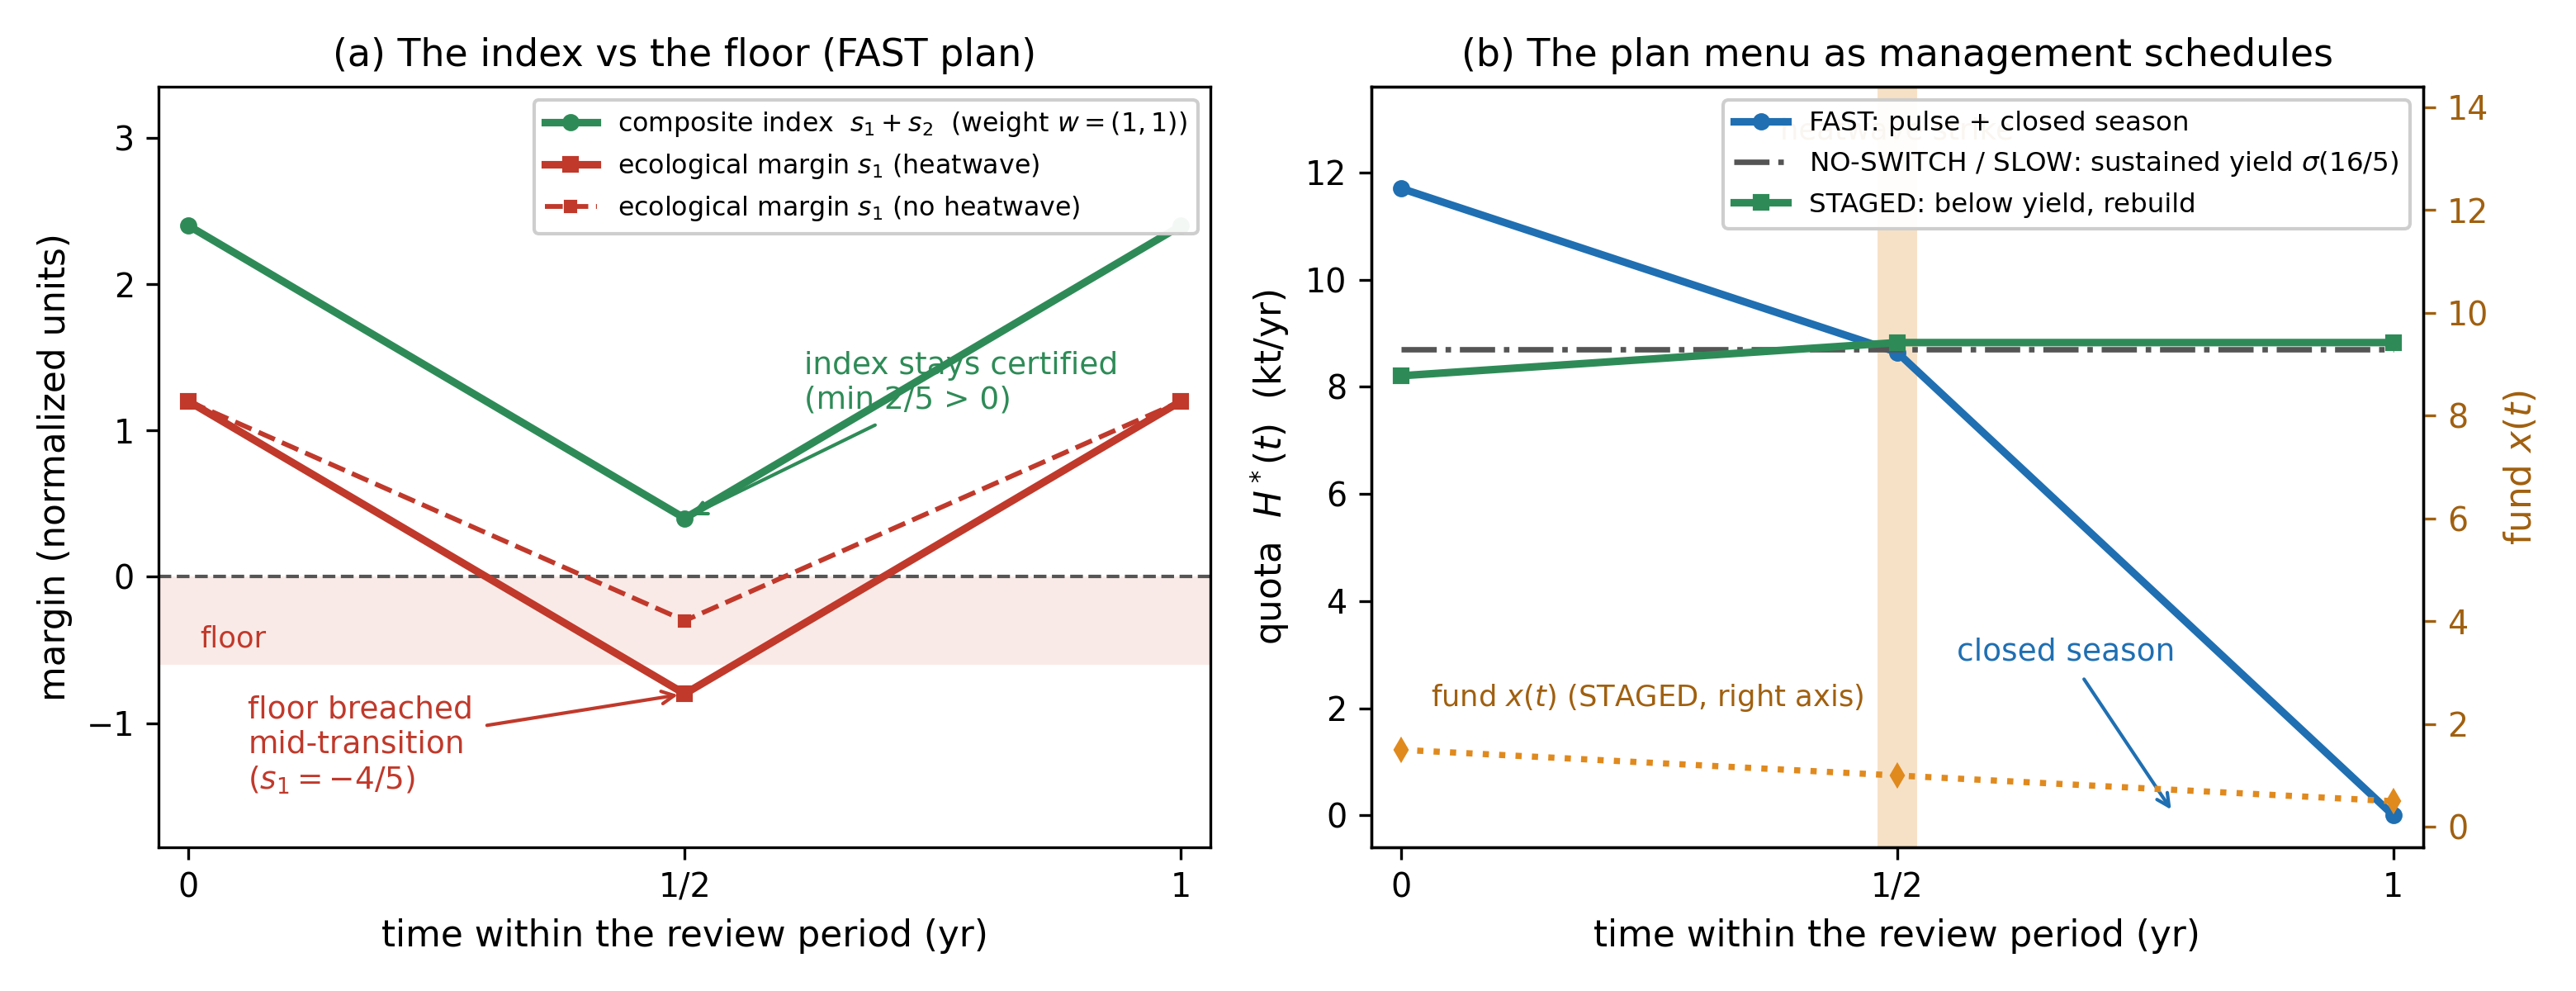
\includegraphics[width=0.98\linewidth]{figs_p1/fig_benchmark_v44.png}
\caption{The witness datum realized as a fishery-transition benchmark
(Section 6.3). (a) Under the pulse-and-closure plan, the composite index
\(s_1 + s_2\) at \(w = (1, 1)\) remains certified at every instant (minimum
\(2/5\)), while the ecological margin breaches its floor mid-transition
(\(-4/5\) under the heatwave strike, \(-3/10\) without it): the
accepted-at-every-weighting reading is blind to the breach. (b) The plan menu
as management schedules: pulse plus closed season; sustained-yield status
quo; and the reserve-financed staged transition, which rebuilds the stock
while improving both margins (the rescue set). All quota, stock, margin, and
fund values are the exact rational values verified in Section 6.3.}
\label{fig:benchmark}
\end{figure}

\subsection{A resource-transition benchmark}\label{resource-transition-benchmark}

The witness datum of Section 4.5 is deliberately spare: a fund, two typed
floors, four plans, and a tube semantics. This section realizes the same
datum as a standard biomass--yield resource model, so that the reader can
read every symbol as a quantity a resource agency actually monitors, and so
that the theorems can be seen to bite on a textbook dynamical system rather
than on a discrete datum alone. The instantiation is an exact rational re-reading of the witness
datum in the domestic language of a Schaefer (1954) production model:
every number below is re-derivable from the deposited benchmark script,
which verifies it in exact rational arithmetic, and the certified tubes
are conservative for the nonlinear realization by an exact inequality. It
is not a fitted case study, and no empirical claim is made.

\textbf{The system.} Let \(B(t)\) denote spawning biomass (kt) in a
stock-specific fishery over one annual review period \(t \in [0, 1]\), with
logistic surplus production
\(\sigma(B) = r B (1 - B/K)\) at \(r = 4\), \(K = 10\), and a biomass limit
\(B_{\mathrm{lim}} = 2\) kt below which the spawning stock is judged unable
to sustain recruitment. The ecological floor is the margin
\(s_1(t) = B(t) - B_{\mathrm{lim}} \ge 0\); the income floor
\(s_2(t) \ge 0\) is the fleet income margin net of costs, maintained by the
quota and by the transition reserve \(x(t)\), an adjustment fund financing
fleet draw-down. Four plans are available, standard in transition management:
\textbf{NO-SWITCH} (status-quo harvest), \textbf{FAST} (an immediate large
quota cut --- a pulse season followed by a closure --- accepting a
mid-season trough on the ecological floor, the plan's certified
exposure), \textbf{SLOW} (a gradual reduction, shifting the burden onto
the income floor), and \textbf{STAGED} (a
below-sustained-yield quota while the reserve finances the fleet transition,
after which both margins improve). Disturbances are environmental shocks: a
mid-season heatwave strike (\(t = 1/2\)) imposing an excess mortality
\(\delta_0 = 1/2\) kt on the stock, present or absent. The state is observed
only through the institutional dashboard, the weighted aggregate
\(w \cdot (s_1, s_2)\), and the reviewer checks the dashboard, not the
floors. This is a deliberately adverse reporting architecture, adopted to
isolate the assessment-operator issue --- not a claim about current
fisheries assessment practice, in which a limit-reference-point breach
triggers a mandatory management response.

\textbf{The datum, domesticated.} At the datum's initial state
\((x, s_1, s_2) = (1/2, 6/5, 6/5)\) --- a half-financed fund, a stock
\(B = B_{\mathrm{lim}} + 6/5 = 16/5\) kt (\(6/5\) kt \(= 1.2\) above the limit), and a
healthy income margin --- the plan menu of Section 4.5 reads: \textbf{FAST}
cuts the quota hard for half a season; with the income floor protected by its
quota schedule, FAST's exposure is the ecological floor, whose worst-case
(dip \(2\)) trajectory is \(s_1\): \(6/5 \to -4/5 \to 6/5\) --- the stock
troughs at \(B_{\mathrm{lim}} + (-4/5) = 6/5\) kt, i.e.\ \(4/5\) kt
\emph{below} the limit (\(s_1 = 6/5 - 2 = -4/5\) relative to the floor).

\textbf{SLOW} mirrors the exposure onto the income floor
(\(s_2: 6/5 \to -4/5 \to 6/5\)). \textbf{STAGED} spends the fund at the
buy-back cost \(c = 1\) while both margins improve by the destination gain
\(e = 1/4\). These are exactly the tube tables verified in Section 4.5 and
in the deposited artifact; the interpretation is new, the arithmetic is not.

\textbf{The benchmark schedule, exactly.} The FAST plan is realized by the
announced quota \(H^*(t)\) that makes the benign margin line
\(s_1\): \(6/5 \to 6/5 - 3/2 \to 6/5\) --- the tube-table line with the
heatwave's \(1/2\)-kt dip removed --- an exact trajectory
of \(\dot B = \sigma(B) - H^*(t)\): on \((0, 1/2)\),
\(H^* = 3 + \sigma(B_{\mathrm{line}}(t))\) (a pulse declining from
\(\tfrac{1463}{125} \approx 11.7\) to \(\tfrac{2161}{250} \approx 8.6\) kt/yr
--- admissible against the fleet capacity \(H_{\max} = 13\)), and on
\((1/2, 1)\) a closure, \(H^* = 0\). The benign branch then tracks the tube
line exactly. The heatwave strike at \(t = 1/2\) drops the stock by
\(\delta_0\), from the trough \(17/10\) kt to \(6/5\) kt --- the adverse
tube's value --- and the closure lets the surplus rebuild the stock: on the adverse
recovery leg the surplus is at least \(\sigma(6/5) = 528/125 > 4\) kt/yr,
while the certified recovery needs only \(4\), so the realized nonlinear
trajectory lies on or above the certified tube throughout; the certified
tubes are conservative for the Schaefer realization.

The remaining plans are
read off the same model: NO-SWITCH and SLOW hold \(B = 16/5\) at the
sustained-yield quota \(\sigma(16/5) = 1088/125 \approx 8.7\) kt/yr ---
itself below the model's maximum sustainable yield (MSY) of
\(\sigma(K/2) = rK/4 = 10\) kt/yr at \(B = K/2\); STAGED
(entered at the rescue witness, fund \(x = 3/2\)) taxes the sustained yield
by the margin improvement, rebuilding the stock
\(16/5 \to 69/20\) while the fund draws down \(3/2 \to 1/2\) and both typed
margins improve by \(e = 1/4\).

\textbf{The dashboard reading.} Under the heatwave branch of the
licensed plan, the composite index at the equal weighting, \(s_1 + s_2\),
has the tube values \((12/5, 2/5, 12/5)\): the dashboard never drops below
\(2/5\), and the transition is certified at \emph{every} weighting
(Section 4.5's per-weight thresholds \(\rho_1 = 2/3\), \(\rho_2 = 3/2\) place
FAST inside every assessor's acceptance set at income-heavy weights and SLOW
inside every assessor's at biomass-heavy weights, with their overlap
containing \(r = 1\)). The floor itself, meanwhile, is breached
mid-transition on both branches (\(-4/5\) with the strike, \(-3/10\)
without), and no plan in the menu keeps both floors path-wise --- the
aggregate dashboard certifies a transition that violates the biomass limit
on both branches --- with the strike and without it --- and no weighting
can detect this from the index alone.

The reserve threshold is the operational number: a fund below
the buy-back cost \(c = 1\) makes the staged transition
unfinanceable (\(\kappa^*(z) = 1 - x\) at the stricken states), so every
state of the failure set \(\{x < 1,\, s_1 < 2,\, s_2 < 2\}\) carries
the finite shortfall \(\kappa^* = 1 - x\); the impossibility region is
its part that the dashboard still certifies, and a modest top-up of the
adjustment fund converts it into a rescue state. In
management language: the dashboard is structurally unable to distinguish a
transition that survives the heatwave from one that does not, and the
financing gap, not the weighting, is what separates them
(Figure~\ref{fig:benchmark}).

\medskip

\noindent Table~\ref{tab:fisheries} completes the translation guide of
Table~\ref{tab:translation} into the benchmark's own vocabulary: each of
the paper's central objects read as the fisheries quantity of this
section.

\begin{table}[htbp]
\centering
\small
\caption{The translation guide (Table~\ref{tab:translation}) extended to
the fishery benchmark's own quantities.}
\label{tab:fisheries}
\begin{tabular}{@{}p{4.1cm}p{9.4cm}@{}}
\toprule
Object & Fisheries reading (this section) \\
\midrule
Typed floors \(s_i \ge 0\) & the spawning-stock margin above the limit reference point (\(B - B_{\mathrm{lim}} \ge 0\); the LRP convention) and the fleet income margin net of costs \\
Scalarized operator \(E_w\) & the assessment dashboard \(w \cdot (s_1, s_2)\) the reviewer checks \\
Licensing thresholds \(\rho_1, \rho_2\) & weight-ratio licensing intervals for the pulse (FAST) and gradual (SLOW) quota plans \\
Acceptance gap \(\mathrm{FP}_{\mathrm{agg}}\) & dashboard-certified yet LRP-breaching transitions (the index-blindness zone: trough \(0.6\) LRP units while the dashboard reads \(2/5 > 0\)) \\
Rescue set \(R\); threshold \(\kappa^*\) & the adjustment fund financing fleet buy-down (STAGED at cost \(c = 1\); the shortfall \(\kappa^* = 1 - x\)) \\
Impossibility region \(I\) & underfunded transitions: fund \(x < 1\), both margins below their plan margins, dashboard still certified \\
Blend collapse vs.\ time-sharing & fractional quota/effort allocation (convexification) vs.\ pulse/gradual season alternation \\
Exact-tube semantics & no transient LRP breach along the transition, the mid-season heatwave included \\
\bottomrule
\end{tabular}
\end{table}


\textbf{A data anchor on a real stock.} The benchmark's units are not chosen in a
vacuum: they are anchored to a real, regulated floor. For Northern cod
(\emph{Gadus morhua}, NAFO Divisions 2J3KL), the assessed spawning-stock
series (NCAM M-shift, 1983--2015) carries a limit reference point (LRP) of
\(884.6\) kt (DFO, 2016) --- the biomass below which recruitment is judged
impaired; the same series underlies the companion scored test of
surplus-production forecasters on this stock (Abaee, 2026, \emph{Does a
Surplus-Production Ladder Improve Forecasts of Northern Cod?}). Reading the
benchmark's floor as this LRP fixes the dashboard arithmetic: the witness's
opening stock (\(1.6\) LRP units, \(1.6 \times 884.6 \approx 1.42\) Mt) is the
neighbourhood of the assessed mid-1980s Northern cod spawning biomass, the
adverse plan's trough (\(B = 6/5\) kt, \(0.6\) LRP units \(\approx 531\)
kt) lies below the LRP while remaining above the stock's 2015
assessed level of about a third of the LRP (\(33.8\%\), \(\approx 299\)
kt; DFO, 2016) --- the zone between the two levels, in which the stock in fact
resided after the collapse --- and the adverse plan's
worst-case stock excursion --- \(2\) kt, i.e.\ one full LRP unit (the
quota's \(3/2\)-kt draw-down plus the heatwave's \(1/2\)-kt excess
mortality) --- is the order of the stock's swing across the LRP itself.
\textbf{The motivation, with the assessed numbers.} The anchoring
statements of this subsection, made precise: the limit reference point of
the assessed NCAM M-shift series is \(884.6\) kt --- by construction the
1983--1989 mean spawning-stock biomass of that series (DFO, 2016, Table
A2); the stock's assessed 2015 level is \(33.8\%\) of that LRP (the
advisory report's ``about a third''), \(\approx 299\) kt; the decline
from the mid-1980s neighbourhood of the benchmark's opening stock
(\(\approx 1.42\) Mt) to the 2015 level is a swing of \(\approx 1.1\)
Mt, about \(1.3\) LRP units; and the benchmark's adverse worst-case
excursion --- one full LRP unit --- is therefore of the assessed order,
with its trough (\(0.6\) LRP) inside the assessed post-collapse band
\((0.34, 1)\) LRP units. The unit convention is explicit throughout:
\(s_1\) is a kt margin above \(B_{\mathrm{lim}}\), so the opening
stock is \(B(0) = B_{\mathrm{lim}} + 6/5 = 16/5\) kt, the normalized
stock is \(b(0) = B(0)/B_{\mathrm{lim}} = 8/5 = 1.6\) LRP units, and the
margin \(6/5\) kt is not itself a biomass ratio.

Three qualifications apply. The anchoring fixes units only: no
parameter of the rational witness is estimated from data, and the
theorems say nothing predictive about this or any other stock. And the companion scored test adds a caution of exactly the
discipline this paper practises: on the same series, no structural
surplus-production model in the scored ladder beat last-value persistence
(one-year RMSE \(98\) kt versus \(115\)--\(206\) kt), and every model missed
the collapse window --- what survives institutional scrutiny on such a stock
is the menu and the floors, both of which are set by management and both of
which this paper's datum takes as given, rather than a predictive fit of the
dynamics.

\begin{center}\rule{0.5\linewidth}{0.5pt}\end{center}

\section{Conclusions}\label{conclusions}

Scalarized and coordinate-wise feasibility criteria are usually compared
as doctrines --- as different normative stances on substitutability, of
which the weak- and strong-sustainability traditions are the canonical
instances. This paper shows that the divergence between the two criteria
as formalized here --- the scalarized-aggregate and typed
operators of Section 3.1 on a common action menu and disturbance class
--- survives translation into assessment mechanics, at the level of a
theorem about those operators. The theorem establishes no ranking of doctrines: Section 5.1 delimits the formalizations, and by Theorem 9 the structural character of the separation is a property of the finite deterministic menu, not of either tradition (Sections 4.10--4.11). On a typed transition datum under exact-tube semantics, the
compensatory reading (per-weight acceptance) and the noncompensatory
reading (common-plan acceptance) are related by a quantifier commutation
that can fail on an open region of state space. Where it fails, every
scalarization weight certifies a transition, but no single transition is
certified by all weights, and the certified set splits into states
rescuable by a resource-controlled action and states that are impossible
under every weight. The mechanism is not scalarization blindness --- at
fixed trajectories the full-cone aggregate is lossless --- but the
policy dependence of the aggregate-feasible transition. The
finite-menu theorem of Section 4.4 states the underlying mechanism in
full generality: for any finite menu, the acceptance gap is the part of
the convex hull of the required margins that no single plan dominates,
so the witness of Section 4.5 is an instance of a geometric fact rather
than an isolated construction.

For the construction of composite sustainability indices, the theorem
has a concrete consequence. An index can be sound at the level of
accounting and still over-certify at the level of assessment, because
certification is a quantifier statement about transitions, not a
property of a number. Where separately-binding floors matter, per-floor
reporting is not a presentation preference but a detection requirement:
the aggregate alone cannot distinguish the rescue region from the
impossibility region. The bridge a composite index needs --- some single
transition that serves every admissible weight, i.e.~membership in
\(\mathcal{V}_{\mathrm{typ}}\) --- is exactly what the frameworks'
reporting conventions should be asked to exhibit. Theorem 9 qualifies this requirement: such a single transition is not, in general, a member of the specified deterministic menu but a convexified action, so the relevant question for a reporting convention is whether its action set admits the required menu convexification --- and Proposition 10 shows that temporal alternation alone does not provide it.

\section*{List of abbreviations}\label{list-of-abbreviations}

\begin{itemize}
\item \textbf{CES} --- constant elasticity of substitution
\item \textbf{MSY} --- maximum sustainable yield
\item \textbf{PROMETHEE} --- Preference Ranking Organisation Method for Enrichment Evaluation
\end{itemize}

\begin{center}\rule{0.5\linewidth}{0.5pt}\end{center}


\appendix

\section{Proofs of the general results}

\textbf{Proof of Remark 1 (Section 4.1).}\ If \(a \in \bigcap_\lambda E_\lambda(z)\), then each
\(E_\lambda(z)\) is nonempty, so \(z\) lies in the right-hand set. The
inclusion fails at \(z\) precisely when each \(E_\lambda(z)\) is
nonempty but \(\bigcap_\lambda E_\lambda(z) = \varnothing\), i.e.~when
no common selector exists; this is the stated equality condition. \ensuremath{\square}

\textbf{Proof of Remark 2 (Section 4.2).}\ (\(\Rightarrow\)) \(w \ge 0\), \(w \neq 0\), \(v \ge 0\)
gives \(w \cdot v = \sum_i w_i v_i \ge 0\). (\(\Leftarrow\)) If
\(v_k < 0\), take \(w = e_k \in W_+\): then \(w \cdot v = v_k < 0\). \ensuremath{\square}

\textbf{Proof of Proposition 3 (Section 4.3).}\ (i) Let \(a \in E_{\mathrm{typ}}(z)\). For every
disturbance \(d\),
\(\mathrm{Tube}(a,d) \subseteq S = S^{\mathrm{phys}} \cap \{s \ge 0\}\).
By Remark 2, every tube point satisfies \(w \cdot s \ge 0\) for every
\(w \in W_+\), and likewise every successor state lies in \(G^w\); hence
\(a \in E_w(z)\). The remaining inclusions follow from
\(S^w \subseteq S^{\mathrm{phys}}\),
\(G^w \subseteq G^{\mathrm{phys}}\), and
\(\mathrm{End}(a,d) \subseteq \mathrm{Tube}(a,d)\). (ii) The inclusion
\(\subseteq\) is part (i) intersected over \(w\). For the reverse
inclusion, let \(a \in \bigcap_{w \in W_+} E_w(z)\). For every \(d\) and
every tube point \(p \in \mathrm{Tube}(a,d)\), every \(w \in W_+\) gives
\(w \cdot s(p) \ge 0\), so by Remark 2 \(s(p) \ge 0\) componentwise;
hence \(\mathrm{Tube}(a,d) \subseteq S\). The same argument with
\(\mathrm{Succ}\) gives \(\mathrm{Succ}(a,d) \subseteq G\). Thus
\(a \in E_{\mathrm{typ}}(z)\). \ensuremath{\square}

\textbf{Proof of Proposition 4 (Section 4.4).}\ For the second inclusion: by Proposition 3(i),
\(E_w(z) \subseteq E_{\mathrm{tube,phys}}(z)\) for every \(w\), so
\(\mathcal{V}_w \subseteq \mathcal{V}_{\mathrm{phys}}\), and
intersecting over \(w \in W\) preserves the inclusion. For the first: if
\(z \in \mathcal{V}_{\mathrm{typ}}\), then by Proposition 3(ii) there
exists \(a \in \bigcap_{w \in W_+} E_w(z)\); this same \(a\) lies in
\(\bigcap_{w \in W} E_w(z)\), so \(E_w(z) \neq \varnothing\) for every
\(w \in W\), i.e.~\(z \in \mathcal{V}_W\). Monotonicity: intersecting
over a larger family can only shrink the intersection. \ensuremath{\square}

\textbf{Proof of the finite-menu theorem (Section 4.4).}\ (i) is the margin test restated. For (ii), if
\(s = d + v\) with \(d \in \operatorname{conv}(\mathcal{D})\) and \(v \ge 0\), then
for every \(w \ge 0\), \(w \cdot s \ge w \cdot d \ge \min_a w \cdot d_a\),
so the scalarized test holds. Conversely, suppose
\(s \notin \operatorname{conv}(\mathcal{D}) + \mathbb{R}^n_+\); this set is closed
and convex (a compact polytope plus a closed cone), so strict separation
gives \(w \ne 0\) with \(w \cdot s < w \cdot d + w \cdot v\) for every
\(d \in \operatorname{conv}(\mathcal{D})\) and every \(v \ge 0\). Since \(v\)
ranges over the whole cone, \(w \in \mathbb{R}^n_+ \setminus \{0\}\), and
taking \(v = 0\) gives
\(w \cdot s < \min_{d \in \operatorname{conv}(\mathcal{D})} w \cdot d =
\min_a w \cdot d_a\): the scalarized test fails. \ensuremath{\square}

\section{Proofs for the witness datum}

\textbf{Proof of Theorem 5 (Section 4.6).}\ \textbf{(1)} Typed admissibility requires the worst-case
tube in \(S_0\) and the successor in \(G\). NO-SWITCH never reaches
\(G\) (its successor retains \(q = 0\)), so it is never admissible. For
FAST, the worst-case \(s_1\)-tube is \([s_1 - 2, s_1]\), safe if and
only if \(s_1 \ge 2\); its successor \((1, x, s + e)\) lies in \(G\)
given \(x \ge 0\). Hence FAST is typed-admissible exactly when
\(s_1 \ge 2\). Symmetrically, SLOW is typed-admissible exactly when
\(s_2 \ge 2\). For STAGED, the floors grow through the interval and the
successor lies in \(G\); the binding constraint is the \(x\)-tube
\([x - 1, x]\), safe if and only if \(x \ge 1\). Therefore
\(E_{\mathrm{typ}}(z) \neq \varnothing\) exactly on
\(\{x \ge 1\} \cup \{s_1 \ge 2\} \cup \{s_2 \ge 2\}\).

\textbf{(2)} Fix \(w = (w_1, w_2) \in W_+\). NO-SWITCH misses \(G^w\)
and is never admissible. FAST is \(w\)-admissible if and only if its
worst-case aggregate value stays nonnegative:
\(w_1(s_1 - 2) + w_2 s_2 \ge 0\), i.e.~\(w_1 s_1 + w_2 s_2 \ge 2 w_1\)
(automatic when \(w_1 = 0\)). Symmetrically SLOW is \(w\)-admissible if
and only if \(w_1 s_1 + w_2 s_2 \ge 2 w_2\). STAGED is \(w\)-admissible
if and only if \(x \ge 1\) (the physical constraint within \(S^w\)),
since \(w \cdot s \ge 0\) holds automatically along its tube. Hence
\(z \in \mathcal{V}_w\) whenever \(x \ge 1\); and if \(x < 1\), then
\(z \in \mathcal{V}_w\) if and only if at least one of the two
inequalities above holds.

Suppose first \(x \ge 1\): then \(z \in \mathcal{V}_w\) for every \(w\),
so \(z \in \mathcal{V}_{\mathrm{weak}}\). Suppose \(x < 1\) and
\(s_1 \ge 2\) or \(s_2 \ge 2\): say \(s_1 \ge 2\); then FAST is
typed-admissible by (1), hence \(w\)-admissible for every \(w\), so
\(z \in \mathcal{V}_{\mathrm{weak}}\). It remains to treat \(x < 1\)
with \(s_1 < 2\) and \(s_2 < 2\). For \(w_1 > 0\), write
\(r = w_2/w_1\): FAST is \(w\)-admissible exactly when
\(s_1 + r s_2 \ge 2\), i.e.~\(r \ge (2 - s_1)/s_2 = \rho_1\) (using
\(s_2 > 0\); when \(s_2 = 0\) the condition reduces to \(s_1 \ge 2\),
which is excluded). SLOW is \(w\)-admissible exactly when
\(s_1 + r s_2 \ge 2r\), i.e.~\(r \le s_1/(2 - s_2) = \rho_2\) (using
\(s_2 < 2\)). The boundary weights are the same limiting cases: at
\(w_1 = 0\) (\(r \to \infty\)) FAST is licensed provided \(s_2 \ge 0\),
while SLOW is strictly rejected on the region \(s_2 < 2\);
symmetrically, at \(w_2 = 0\) (\(r = 0\)) SLOW is licensed provided
\(s_1 \ge 0\), while FAST is rejected on the region \(s_1 < 2\).
Therefore \(z \in \mathcal{V}_w\) for every \(w \in W_+\) if and only if
the intervals \(\{r \ge \rho_1\}\) and \(\{r \le \rho_2\}\) together
cover all of \([0, \infty]\), which holds exactly when
\(\rho_2 \ge \rho_1\). Computing,
\[\rho_2 \ge \rho_1 \iff \frac{s_1}{2 - s_2} \ge \frac{2 - s_1}{s_2} \iff s_1 s_2 \ge (2 - s_1)(2 - s_2) \iff s_1 + s_2 \ge 2,\]
with both denominators positive in the present case. Hence, in this
case, \(z \in \mathcal{V}_{\mathrm{weak}}\) if and only if
\(s_1 + s_2 \ge 2\). Assembling the three cases, and noting
\(\{s_1 \ge 2\} \cup \{s_2 \ge 2\} \subseteq \{s_1 + s_2 \ge 2\}\) under
nonnegativity,
\[\mathcal{V}_{\mathrm{weak}} = \{ x \ge 1 \} \cup \{ s_1 + s_2 \ge 2 \}.\]

\textbf{(3)} In the physical operators the only constraint is
\(x \ge 0\) (with \(q = 1\) at the destination). FAST and SLOW have
tubes within \(S^{\mathrm{phys}}\) and successors in
\(G^{\mathrm{phys}}\) for every \(z \in X_0\) (their dips affect only
\(s\), which is unconstrained physically); STAGED does so exactly for
\(x \ge 1\). Hence \(E_{\mathrm{tube,phys}}(z) \neq \varnothing\) for
every \(z \in X_0\), so \(\mathcal{V}_{\mathrm{phys}} = X_0\). For the
endpoint operator, the endpoint values of FAST and SLOW lie in
\(S^{\mathrm{phys}}\) for every \(z \in X_0\), so
\(\mathcal{V}_{\mathrm{end}} = X_0\) as well.

\textbf{(4)} By (1)--(2),
\[\mathrm{FP}_{\mathrm{agg}} = \mathcal{V}_{\mathrm{weak}} \setminus \mathcal{V}_{\mathrm{typ}}
= \big[ \{x \ge 1\} \cup \{s_1 + s_2 \ge 2\} \big] \setminus \big[ \{x \ge 1\} \cup \{s_1 \ge 2\} \cup \{s_2 \ge 2\} \big]\]
\[= \{ x < 1,\ s_1 < 2,\ s_2 < 2,\ s_1 + s_2 \ge 2 \} = I.\]
This set is nonempty
(e.g.~\((x, s_1, s_2) = (\tfrac12, \tfrac65, \tfrac65)\)), and its
relatively open interior is the stated region.

\textbf{(5)} By (4),
\(I = \mathrm{FP}_{\mathrm{agg}} = \mathcal{V}_{\mathrm{weak}} \setminus \mathcal{V}_{\mathrm{typ}} \neq \varnothing\),
so the first inclusion is strict. For the second, the point
\((\tfrac12, \tfrac1{10}, \tfrac1{10})\) satisfies \(x < 1\) and
\(s_1 + s_2 = \tfrac15 < 2\), so it lies outside
\(\mathcal{V}_{\mathrm{weak}}\) by (2), while by (3) it lies in
\(\mathcal{V}_{\mathrm{phys}}\).

\textbf{(6)} The threshold characterization was derived in the proof of
(2): with \(r = w_2 / w_1\), FAST is licensed exactly for
\(r \ge \rho_1\) and SLOW exactly for \(r \le \rho_2\), and
\(\rho_2 \ge \rho_1 \iff s_1 + s_2 \ge 2\). On \(\mathcal{Q}\) the
inequality \(s_1 + s_2 \ge 2\) holds, so the two licensing intervals
overlap and together cover all weights; strictly on the relative
interior (\(s_1 + s_2 > 2\)) both thresholds are finite and the
intervals overlap in a nondegenerate interval, with \(r > \rho_2\)
licensing FAST only and \(r < \rho_1\) licensing SLOW only. On \(I\)
(where \(x < 1\)), STAGED is inadmissible for every \(w\), so
\(E_{\mathrm{typ}}(z) = \bigcap_w E_w(z) = \varnothing\) by Proposition
3(ii): no single action serves every weight. On \(R\) (where
\(x \ge 1\)), STAGED lies in \(E_{\mathrm{typ}}(z) = \bigcap_w E_w(z)\)
and serves every weight.

\textbf{(7)} On \(R\), STAGED's tube is
\([x - 1, x] \times \{s \to s + e\}\): the \(x\)-tube stays nonnegative
because \(x \ge 1\), the floors grow, and the successor
\((1, x - 1, s + e) \in G\). On \(I\), the four exhibited violations
exhaust the action set and each violates a typed constraint: FAST's
\(s_1\)-tube reaches \(s_1 - 2 < 0\); SLOW's \(s_2\)-tube reaches
\(s_2 - 2 < 0\); STAGED's \(x\)-tube reaches \(x - 1 < 0\); NO-SWITCH's
successor misses \(G\). \ensuremath{\square}

\textbf{Proof of Remark 7 (Section 4.8).}\ (i) Backward induction on stages. Base: at the final stage
the terminal sets satisfy
\(G \subseteq G^w \subseteq G^{\mathrm{phys}}\) by Remark 2 and the
definition of the terminal sets. Step: the accepted set of a stage is
the set of states from which some action keeps the tube in the safe set
and the successor in the next-stage accepted set; applying Proposition
3(i) to the stage's action sets and the induction hypothesis to the
next-stage accepted sets preserves the three-way inclusion at the stage
level. (ii) With HOLD the unique prefix action, a prefix state is
accepted exactly when it lies in the prefix safe set and in the
next-stage accepted set; the stage-0 regions are therefore the witness
regions of Theorem 5 pulled back through the (identity) holds, and the
strictness witnesses (\(I \neq \varnothing\) and the point
\((\tfrac12, \tfrac1{10}, \tfrac1{10})\)) persist. (iii) The three
listed mechanisms are each sufficient to erase the gap in a multi-stage
setting, so no unconditional generalization is asserted. \ensuremath{\square}

\textbf{Proof of Theorem 8 (Section 4.8).}\ \emph{Datum.} Two capital forms, floors at zero, the bridge stock absent
(\(x \equiv 0\)); states are pairs \(s = (s_1, s_2)\). Stage 2 (final
interval): safe set \(S_0^{(2)} = \mathbb{R}^2\) (no path constraint),
terminal sets \(G^{(2)} = G^{w,(2)} = G = \{ s \ge 0 \}\) --- coincident
for every weight --- and a single action REPAIR with tube \(\{s\}\)
(safe trivially) and successor \((1, 1) \in G\). Stage 1: safe set
\(S_0 = \{ s \ge 0 \}\); two actions with constant tubes, safe at every
state of \(S_0\): A1 with successor \((s_1 - 1, s_2 + 1)\) and A2 with
successor \((s_1 + 1, s_2 - 1)\); the stage-1 terminal architecture is
the stage-2 accepted sets. Initial state \(z^* = (\tfrac25, \tfrac25)\).

\emph{In the two-stage datum the gap is erased.} REPAIR is
typed-admissible --- hence \(w\)-admissible for every weight --- from
every state, so
\(\mathcal{V}_{\mathrm{typ}}^{(2)} = \mathcal{V}_w^{(2)} = \mathbb{R}^2\)
for every \(w\): the stage-2 accepted sets coincide. Backward induction
then admits both A1 and A2 at \(z^*\) (safe tubes; successors in
\(\mathcal{V}_{\mathrm{typ}}^{(2)} = \mathbb{R}^2\)), so \(z^*\) is
typed-accepted at stage 0, and weak acceptance follows from typed
acceptance.

\emph{In the single-interval truncation --- the same stage-1 datum with
the final interval collapsed to its terminal sets, \(G = \{s \ge 0\}\)
and \(G^w = \{w \cdot s \ge 0\}\) --- the gap is present.} Both
successors leave \(G\) (\(s_1 - 1 = -\tfrac35 < 0\) and
\(s_2 - 1 = -\tfrac35 < 0\)), so \(z^*\) is typed-rejected. For the weak
doctrine, writing \(r = w_2 / w_1\) on the interior of the weight cone:
A1 is \(w\)-admissible exactly when \((s_1 - 1) + r (s_2 + 1) \ge 0\),
i.e.~\(r \ge \tfrac{1 - s_1}{s_2 + 1} = \tfrac37\); A2 exactly when
\((s_1 + 1) + r (s_2 - 1) \ge 0\),
i.e.~\(r \le \tfrac{s_1 + 1}{1 - s_2} = \tfrac73\); the two intervals
cover \([0, \infty]\) because \(\tfrac37 < \tfrac73\), and the boundary
weights are covered directly (\(r = 0\): A2 gives
\(w_1(s_1 + 1) \ge 0\); \(r \to \infty\): A1 gives
\(w_2(s_2 + 1) \ge 0\)). Hence \(z^* \in \mathcal{V}_{\mathrm{weak}}\)
in the truncation, and the gap
\(\mathcal{V}_{\mathrm{weak}} \setminus \mathcal{V}_{\mathrm{typ}}\)
contains \(z^*\). \ensuremath{\square}

\textbf{Proof of Theorem 9 (Section 4.10).}\ (i) FAST's worst-case tube has \(s_1\)-coordinates
\([s_1 - 2, s_1]\) and \(s_2\)-coordinate \(\{s_2\}\); SLOW's has
\(s_1\)-coordinate \(\{s_1\}\) and \(s_2\)-coordinates
\([s_2 - 2, s_2]\); both keep \(x\) nonnegative throughout (their dips
affect only \(s\)). The blended tube therefore has \(s_1\)-coordinates
\([s_1 - 2\delta, s_1]\), \(s_2\)-coordinates
\([s_2 - 2(1-\delta), s_2]\), and nonnegative \(x\)-coordinates (convex
combinations of nonnegative quantities). Typed admissibility requires
the tube within \(S_0 = \{x \ge 0, s \ge 0\}\) and the successor in
\(G\). The tube condition is exactly the displayed window. The successor
is the mixture of the two successors, which the datum fixes to the same
value --- the action table of Section 4.5 gives both FAST and SLOW the
successor \((1, x, s + e)\) --- so the blended successor is
\((1, x, s + e) \in G\): \(x \ge 0\) and the destination label is \(1\).
The window is nonempty exactly when \(1 - s_2/2 \le s_1/2\),
i.e.~\(s_1 + s_2 \ge 2\); on \(\mathcal{Q}\) the raw window already
lies in \((0,1)\) (\(s_1 < 2, s_2 < 2\) give \(0 < 1 - s_2/2\) and
\(s_1/2 < 1\)), so the \([0,1]\) clip in the statement is inactive
there; at equality it is the singleton
\(\delta = s_1/2 = 1 - s_2/2\), feasible because \(S_0\) is closed. On
the boundary faces (\(s_1 = 0\) or \(s_2 = 0\)) the window is closed at
the corresponding endpoint, and the classification follows the boundary
conventions of Section 4.6.

\begin{enumerate}
\def\labelenumi{(\roman{enumi})}
\setcounter{enumi}{1}
\item
  If \(s_1 + s_2 \ge 2\), (i) supplies a typed-admissible blend whatever
  the value of \(x \ge 0\); if \(s_1 + s_2 < 2\), no blend is
  typed-admissible by (i), and the deterministic menu contributes
  exactly
  \(\mathcal{V}_{\mathrm{typ}} = \{x \ge 1\} \cup \{s_1 \ge 2\} \cup \{s_2 \ge 2\} \subseteq \{x \ge 1\} \cup \{s_1 + s_2 \ge 2\}\).
  Hence the augmented typed set equals
  \(\{x \ge 1\} \cup \{s_1 + s_2 \ge 2\} = \mathcal{V}_{\mathrm{weak}}\)
  by Theorem 5(2) --- and nothing beyond, since every admissible blend
  satisfies \(s_1 + s_2 \ge 2\) and the deterministic actions stay
  within \(\mathcal{V}_{\mathrm{typ}}\).
\item
  Immediate from the window's state dependence and from typed
  admissibility implying \(w\)-admissibility for every weight.
\end{enumerate}

\ensuremath{\square}

\textbf{Proof of Proposition 10 (Section 4.11).}\ A sequential policy that spends any positive time on FAST
visits every \(s_1\) in \([s_1 - 2, s_1]\) and any positive time on SLOW
visits every \(s_2\) in \([s_2 - 2, s_2]\); the union tube stays within
\(S_0 = \{x \ge 0, s \ge 0\}\) exactly when both dips are nonnegative,
i.e.~\(s_1 \ge 2\) and \(s_2 \ge 2\). On \(I\) both coordinates are
strictly below 2, so the union tube is never within \(S_0\) and no
sequential policy is typed-admissible; since every member of the finite
deterministic menu is typed-admissible on \(I\) only in the per-weight
sense of Theorem 5(6) (and never in the common sense), the
noncompensatory accepted set does not extend to \(I\) under sequential
time-sharing. \ensuremath{\square}

\section{Proof of the rescue threshold}

\textbf{Proof of the rescue threshold (Section 5.7).}\ Among the augmented menu, only \(\mathrm{STAGED}_\kappa\) depends on \(\kappa\), and its typed-admissibility is independent of the floors: its \(x\)-tube is \([x + \kappa - 1,\; x + \kappa]\), the floors are nondecreasing (they grow to \(s + e\) with \(e = (\tfrac14, \tfrac14) > 0\)), and the successor \((1, x + \kappa - 1, s + e)\) lies in \(G\) exactly when \(x + \kappa - 1 \ge 0\). Hence \(\mathrm{STAGED}_\kappa \in E_{\mathrm{typ}}(z) \iff x + \kappa \ge 1\), for every \(z\). If \(z \in \mathcal{V}_{\mathrm{typ}}\), some base action of \(\mathcal{A} \subseteq \mathcal{A}_\kappa\) is admissible at \(\kappa = 0\), so \(\kappa^*(z) = 0\). If \(z \notin \mathcal{V}_{\mathrm{typ}}\) --- that is, \(x < 1\) and \(s_1 < 2\) and \(s_2 < 2\) --- then NO-SWITCH, FAST, and SLOW all fail (Theorem 5(1)), the only admissible element of \(\mathcal{A}_\kappa\) is \(\mathrm{STAGED}_\kappa\), and it is admissible exactly for \(\kappa \ge 1 - x\); hence \(\kappa^*(z) = 1 - x\). \ensuremath{\square}


\section*{References}\label{references}

Abaee, A. (2026). \emph{An Obstruction Calculus for Viability under Incomplete Observation}. Manuscript submitted for publication.

Abaee, A. (2026). \emph{Does a one-pool water-balance model improve forecasts of Edwards Aquifer head? A scored test at J-17}. Zenodo. \url{https://doi.org/10.5281/zenodo.22552680}.

Abaee, A. (2026). \emph{Does a surplus-production ladder improve forecasts of Northern cod? A scored test on NAFO 2J3KL}. Zenodo. \url{https://doi.org/10.5281/zenodo.22553609}.

Abaee, A. (2026). \emph{How Aggregation Can Conceal Composition: Aggregate Biocapacity and the Identifiability of Modelled Ecological-Capital Drawdown}. Manuscript submitted for publication.

Abaee, A. (2026). \emph{Typed flux ledgers and depletion arithmetic: conservation, componentwise diagnostics, and the semantics of depletion horizons}. Zenodo. \url{https://doi.org/10.5281/zenodo.22554177}.

Abaee, A. (2026). \emph{Verification code and figure pipeline for Aggregate Indices and Transition Safety: A Quantifier-Order Separation Between Scalarized and Coordinate-Wise Feasibility}. figshare. \url{https://doi.org/10.6084/m9.figshare.33764023}.

Asheim, G. B. (1994). Net national product as an indicator of sustainability. \emph{Scandinavian Journal of Economics}, 96(2), 257--265.

Aubin, J.-P. (1991). \emph{Viability Theory}. Birkh\"auser, Boston.

Aubin, J.-P., Bayen, A. M., and Saint-Pierre, P. (2011). \emph{Viability Theory: New Directions}, 2nd ed.~Birkh\"auser, Boston.

Aubin, J.-P., and Catt\'e, F. (2002). Bilateral fixed-points and algebraic properties of viability kernels and capture basins of sets. \emph{Set-Valued Analysis}, 10(4), 379--416.

Becker, W., Saisana, M., Paruolo, P., and Vandecasteele, I. (2017). Weights and importance in composite indicators: Closing the gap. \emph{Ecological Indicators}, 80, 12--22.

Ben-Tal, A., Goryashko, A., Guslitzer, E., and Nemirovski, A. (2004).
Adjustable robust solutions of uncertain linear programs.
\emph{Mathematical Programming}, 99(2), 351--376.

Boos, A. (2015). Genuine savings as an indicator for ``weak''
sustainability: Critical survey and possible ways forward in measuring
weak sustainability. \emph{Sustainability}, 7(4), 4146--4163.

Cairns, R. D., and Martinet, V. (2014). An environmental-economic
measure of sustainable development. \emph{European Economic Review}, 69,
4--17.

Cardaliaguet, P. (1996). A differential game with two players and one target. \emph{SIAM Journal on Control and Optimization}, 34(4), 1441--1460.

Cardaliaguet, P., Quincampoix, M., and Saint-Pierre, P. (1999). Set-valued numerical analysis for optimal control and differential games. In: \emph{Stochastic and Differential Games: Theory and Numerical Methods}, Annals of the International Society of Dynamic Games, vol.~4, Birkh\"auser, Boston, 177--247.

Cinelli, M., Coles, S. R., and Kirwan, K. (2014). Analysis of the
potentials of multi criteria decision analysis methods to conduct
sustainability assessment. \emph{Ecological Indicators}, 46, 138--148.

Daly, H. E. (1990). Toward some operational principles of sustainable
development. \emph{Ecological Economics}, 2(1), 1--6.

Das, I., and Dennis, J. E. (1997). A closer look at drawbacks of
minimizing weighted sums of objectives for Pareto set generation in
multicriteria optimization problems. \emph{Structural Optimization}, 14,
63--69.

Dasgupta, P., and M\"aler, K.-G. (2000). Net national product, wealth, and
social well-being. \emph{Environment and Development Economics}, 5(1),
69--93.

De Lara, M., and Doyen, L. (2008). \emph{Sustainable Management of Natural Resources: Mathematical Models and Methods}. Springer, Berlin.

DFO. (2016). \emph{Stock Assessment of Northern Cod (NAFO Divs. 2J3KL) in 2016}. Canadian Science Advisory Secretariat, Science Advisory Report 2016/026. Fisheries and Oceans Canada, Ottawa.

Doyen, L., and Gajardo, P. (2020). Sustainability standards,
multicriteria maximin, and viability. \emph{Natural Resource Modeling},
33(3), e12250.

Doyen, L., Th\'ebaud, O., B\'en\'e, C., Martinet, V., Gourguet, S., Bertignac, M., Fifas, S., and Blanchard, F. (2012). A stochastic viability approach to ecosystem-based fisheries management. \emph{Ecological Economics}, 75, 32--42.

Ekins, P., Simon, S., Deutsch, L., Folke, C., and De Groot, R. (2003). A
framework for the practical application of the concepts of critical
natural capital and strong sustainability. \emph{Ecological Economics},
44(2), 165--185.

Fabian, M. J., Henrion, R., Kruger, A. Y., and Outrata, J. V. (2010). Error bounds: necessary and sufficient conditions. \emph{Set-Valued Analysis}, 18(2), 121--149.

Fanning, A. L., O'Neill, D. W., Hickel, J., and Roux, N. (2022). The social shortfall and ecological overshoot of nations. \emph{Nature Sustainability}, 5(1), 26--36.

Filippov, A. F. (1988). \emph{Differential Equations with Discontinuous Righthand Sides}. Mathematics and Its Applications (Soviet Series), vol.~18. Kluwer Academic Publishers, Dordrecht.

Fischer, S. M., Joy, M. K., Abrahamse, W., Milfont, T. L., and Petherick, L. M. (2022). The use and misuse of composite environmental indices. \emph{bioRxiv}, 2022.03.15.484501. \url{https://doi.org/10.1101/2022.03.15.484501}.

Frankowska, H. (1989). Optimal trajectories associated with a solution
of contingent Hamilton--Jacobi equations. \emph{Applied Mathematics and
Optimization}, 19, 291--311.

Gao, P., Wang, Y., Wang, H., Song, C., Ye, S., and Wang, X. (2023). A Pareto front-based approach for constructing composite index of sustainability without weights: A comparative study of implementations. \emph{Ecological Indicators}, 155, 110919. \url{https://doi.org/10.1016/j.ecolind.2023.110919}.

Hanley, N., Moffatt, I., Faichney, R., and Wilson, M. (1999). Measuring
sustainability: A time series of alternative indicators for Scotland.
\emph{Ecological Economics}, 28(1), 55--73.

Hickel, J. (2020). The sustainable development index: Measuring the
ecological efficiency of human development in the Anthropocene.
\emph{Ecological Economics}, 167, 106331.

Lade, S. J., Steffen, W., de Vries, W., Carpenter, S. R., Donges, J. F., Gerten, D., Hoff, H., Newbold, T., Richardson, K., and Rockstr\"om, J. (2020). Human impacts on planetary boundaries amplified by Earth system interactions. \emph{Nature Sustainability}, 3(2), 119--128.

Lygeros, J., Tomlin, C., and Sastry, S. (1999). Controllers for
reachability specifications for hybrid systems. \emph{Automatica},
35(3), 349--370.

Martinez-Alier, J., Munda, G., and O'Neill, J. (1998). Weak
comparability of values as a foundation for ecological economics.
\emph{Ecological Economics}, 26(3), 277--286.

Martinet, V. (2011). A characterization of sustainability with
indicators. \emph{Journal of Environmental Economics and Management},
61(2), 183--197.

Nardo, M., Saisana, M., Saltelli, A., Tarantola, S., Hoffmann, A., and Giovannini, E. (2008). \emph{Handbook on Constructing Composite Indicators: Methodology and User Guide}. OECD Publishing, Paris.

Neumayer, E. (2013). \emph{Weak versus Strong Sustainability: Exploring
the Limits of Two Opposing Paradigms}, 4th ed.~Edward Elgar, Cheltenham.

O'Neill, D. W., Fanning, A. L., Lamb, W. F., and Steinberger, J. K. (2018). A good life for all within planetary boundaries. \emph{Nature Sustainability}, 1(2), 88--95.

Raworth, K. (2012). A safe and just space for humanity: Can we live within the doughnut? \emph{Oxfam Policy and Practice: Climate Change and Resilience}, 8(1), 1--26.

Rockstr\"om, J., Steffen, W., Noone, K., et al. (2009). A safe operating
space for humanity. \emph{Nature}, 461, 472--475.

Saint-Pierre, P. (1994). Approximation of the viability kernel.
\emph{Applied Mathematics and Optimization}, 29, 187--209.

Schaefer, M. B. (1954). Some aspects of the dynamics of populations important to the management of commercial marine fisheries. \emph{Inter-American Tropical Tuna Commission Bulletin}, 1(2), 23--56.

Sch\"ar, S., Pohl, E., and Geldermann, J. (2025). Analysing the
compensatory properties of the outranking approach PROMETHEE.
\emph{Journal of Multi-Criteria Decision Analysis}, 32, e70013.

Sion, M. (1958). On general minimax theorems. \emph{Pacific Journal of
Mathematics}, 8(1), 171--176.

Solow, R. M. (1974). Intergenerational equity and exhaustible resources.
\emph{Review of Economic Studies}, 41, 29--45.

Usubiaga-Lia\~no, A. (2025). Strong sustainability in the SEEA and the
wider indicator debate. \emph{One Ecosystem}, 10, e141086.

von Neumann, J. (1928). Zur Theorie der Gesellschaftsspiele.
\emph{Mathematische Annalen}, 100, 295--320.

Warga, J. (1972). \emph{Optimal Control of Differential and Functional Equations}. Academic Press, New York.

World Bank. (2011). \emph{The Changing Wealth of Nations: Measuring
Sustainable Development in the New Millennium}. World Bank, Washington,
D.C.

\begin{center}\rule{0.5\linewidth}{0.5pt}\end{center}

\section*{Supplementary Material}\label{supplementary-material}

Framework extensions (governance constructors, the implementability ladder, the commons obstruction, intergenerational structures, the nested-impossibility theorem, composition interfaces), the planetary-boundaries application note, the full framework definitions, and the conjectures are given in the accompanying Supplementary Material, which also enumerates the machine artifact's 25 checks (S8) and the itemized data requirements for empirical application (S9), and the per-literature positioning notes (S10).

\section*{Declarations}\label{declarations}

\subsection*{Ethics approval and consent to participate}

Not applicable.

\subsection*{Consent for publication}

Not applicable.

\subsection*{Availability of data and materials}

All datasets and code generated and analysed during the current study are available in the figshare repository. The deposit serves two explicit roles: (i) this manuscript's verification artifact --- the exact-integer grid verifier for the finite rational instance (all 25 checks), the figure-generation code, the manuscript figure files, and the preserved novelty-search strings; and (ii) the software companion's archive --- the SafeTransition library (with its own separate 24-check benchmark suite), whose master deposit this shared item also is. The two check lists are distinct and are not pooled. \url{https://doi.org/10.6084/m9.figshare.33764023}

\subsection*{Competing interests}

The authors declare that they have no competing interests.

\subsection*{Funding}

Not applicable.

\subsection*{Authors' contributions}

A.A. conceptualized the entire work, wrote, edited and reviewed the manuscript.

\subsection*{Acknowledgements}

Not applicable.

\subsection*{AI declaration}
GLM (Z.ai), Qwen (Alibaba Cloud) and DeepSeek AI assisted with drafting and iterative review.

\end{document}
